\documentclass{article}
\usepackage{multirow}

% if you need to pass options to natbib, use, e.g.:
%     \PassOptionsToPackage{numbers, compress}{natbib}
% before loading neurips_2020

% ready for submission
% \usepackage{neurips_2020}

% to compile a preprint version, e.g., for submission to arXiv, add add the
% [preprint] option:
%     \usepackage[preprint]{neurips_2020}

% to compile a camera-ready version, add the [final] option, e.g.:
%     \usepackage[final]{neurips_2020}

% to avoid loading the natbib package, add option nonatbib:
     \usepackage[preprint,nonatbib]{neurips_2020}

\usepackage[utf8]{inputenc} % allow utf-8 input
\usepackage[T1]{fontenc}    % use 8-bit T1 fonts
\usepackage{hyperref}       % hyperlinks
\usepackage{url}            % simple URL typesetting
\usepackage{booktabs}       % professional-quality tables
\usepackage{amsfonts}       % blackboard math symbols
\usepackage{nicefrac}       % compact symbols for 1/2, etc.
\usepackage{microtype}      % microtypography
\usepackage{float}
\usepackage{bbm}
\usepackage{amsthm,amsmath,amssymb}
\usepackage{mathtools}
\usepackage{subcaption}
\usepackage{threeparttable}

\usepackage{caption}
\usepackage{tikz}
\usetikzlibrary{arrows,automata, calc, positioning}
\usepackage{adjustbox}
\usepackage{wrapfig}

\usepackage{accents}

\newcommand\munderbar[1]{%
  \underaccent{\bar}{#1}}

\newcommand{\indep}{\raisebox{0.05em}{\rotatebox[origin=c]{90}{$\models$}}}
\DeclareMathOperator*{\argmin}{\arg\!\min}
\DeclareMathOperator*{\argmax}{\arg\!\max}

\newtheorem{proposition}{Proposition}[section]
\newtheorem{definition}{Definition}[section]
\newtheorem{remark}{Remark}[section]
\newtheorem{lemma}{Lemma}[section]
\newtheorem{theorem}{Theorem}[section]
\newtheorem{algorithm}{Algorithm}[section]
\newtheorem{corollary}{Corollary}[section]
\newtheorem{hypothesis}{Hypothesis}[section]
\newtheorem{assumption}{Assumption}[section]
\newtheorem{example}{Example}[section]

\title{Kernel Methods for Causal Functions:
Dose, Heterogeneous, and Incremental Response Curves}

% The \author macro works with any number of authors. There are two commands
% used to separate the names and addresses of multiple authors: \And and \AND.
%
% Using \And between authors leaves it to LaTeX to determine where to break the
% lines. Using \AND forces a line break at that point. So, if LaTeX puts 3 of 4
% authors names on the first line, and the last on the second line, try using
% \AND instead of \And before the third author name.

\author{%
  Rahul Singh \\
  MIT Economics \\
  \texttt{rahul.singh@mit.edu} \\
  % examples of more authors
   \And
   Liyuan Xu \\
Gatsby Unit, UCL \\
   \texttt{liyuan.jo.19@ucl.ac.uk} \\
  % \AND
  % Coauthor \\
  % Affiliation \\
  % Address \\
  % \texttt{email} \\
   \And
   Arthur Gretton \\
   Gatsby Unit, UCL \\
   \texttt{arthur.gretton@gmail.com} \\
  % \And
  % Coauthor \\
  % Affiliation \\
  % Address \\
  % \texttt{email} \\
}

\begin{document}

\maketitle

\begin{abstract}
We propose estimators based on kernel ridge regression for nonparametric causal functions such as dose, heterogeneous, and incremental response curves. Treatment and covariates may be discrete or continuous in general spaces. Due to a decomposition property specific to the RKHS, our estimators have simple closed form solutions. We prove uniform consistency with finite sample rates via original analysis of generalized kernel ridge regression. We extend our main results to counterfactual distributions and to causal functions identified by front and back door criteria. We achieve state-of-the-art performance in nonlinear simulations with many covariates, and conduct a policy evaluation of the US Job Corps training program for disadvantaged youths. 
\end{abstract}


%\rscomment{The target length is 8 pages for the NeurIPS workshop and 13.5 pages for ECMA. The table of contents adds 3.5 pages}

%\tableofcontents

\section{Introduction}\label{sec:intro}

\subsection{Motivation}

Program evaluation aims to measure the counterfactual relationship between treatment $D$ and outcome $Y$, which may vary for different subpopulations: if we intervened on treatment, setting $D=d$, what would be the expected counterfactual outcome $Y^{(d)}$ for individuals with characteristics $V=v$? When treatment is binary, the causal parameter is a function $\theta_0(v)=E\{Y^{(1)}-Y^{(0)} \mid V=v\}$ called the heterogeneous treatment effect; when treatment is continuous, it is a function $\theta_0(d,v)=E\{Y^{(d)} \mid V=v\}$ that we call a heterogeneous response curve. Assuming selection on observable covariates $(V,X)$, the causal function $\theta_0(d,v)$ can be recovered by integrating the regression function $\gamma_0(d,v,x)=E(Y \mid D=d,V=v,X=x)$ according to the conditional distribution $\text{\normalfont pr}(x \mid v)$: $\theta_0(d,v)=\int \gamma_0(d,v,x)\mathrm{d}\text{\normalfont pr}(x \mid v)$ \cite{rosenbaum1983central,robins1986new}, which may be complex when there are many covariates. 

The same is true for other causal functions such as dose
%$\theta_0(d,v)=E[Y^{(d)} \mid V=v]$ 
and incremental response curves, 
%$\theta_0(d)=E[\nabla_d Y^{(d)}]$, 
and even counterfactual distributions, albeit with different regressions and reweightings. Therefore nonparametric estimation of a causal function involves three challenging steps: estimating a nonlinear regression, with possibly many covariates; estimating the distribution for reweighting, which may be conditional; and using the nonparametric distribution to integrate the nonparametric regression. For this reason, flexible estimation of nonparametric causal functions, such as $\theta_0(d,v)$, is often deemed too computationally demanding to be practical for program evaluation. %See Section~\ref{sec:related} for a discussion of related work.

%\cite{kennedy2017nonparametric,semenova2021debiased,nie2021quasi,kallus2018policy,chernozhukov2018global,fan2019estimation,zimmert2019nonparametric,colangelo2020double} 

% Additional nuanced questions can be asked. Is the causal relationship between treatment and outcome learned in one population externally valid in another? For the subpopulation who received one treatment value, what would have been their outcome had they instead received another? Are treatment effects heterogeneous with respect to some interpretable subcovariate $V\subset X$ such as age, race, or gender? Such empirical questions are ubiquitous in policy evaluation across economics, statistics, and epidemiology.

Our key insight is that the reproducing kernel Hilbert space (RKHS), a popular nonparametric setting in machine learning, is precisely the class of functions for which the steps of nonparametric causal estimation can be separated. This decomposition follows almost immediately from the definition of the RKHS, and it is a specific strength of our framework; random forests, for example, do not allow such decoupling. Our key insight follows from a more fundamental one. Evaluation of a causal function is generally not a bounded functional over all of $\mathbb{L}^2$ \cite{van1991differentiable,newey1994asymptotic}. We prove that the evaluation of a causal function is a bounded functional over the RKHS $\mathcal{H}$, which is a subset of $\mathbb{L}^2$. By the classic Riesz representation theorem of functional analysis, a bounded functional over a Hilbert space admits a decoupled inner product representation within the Hilbert space. We show how to use this representation to separate the steps of nonparametric causal estimation. This insight appears to be original.

We adapt kernel ridge regression, a classic machine learning algorithm that generalizes splines \cite{wahba1990spline}, to address the computational challenges of estimating causal functions such as dose, heterogeneous, and incremental response curves. Nonparametric estimation with kernels is quite simple: the nonlinear regression with many covariates can be estimated by simple matrix operations; the conditional distribution can be expressed as a regression problem and estimated by simple matrix operations as well; and the step of integration can be performed by taking the product of the results. The final nonparametric estimator for the causal function has a one line, closed form solution, unlike previous work. This simplicity makes the family of estimators highly practical. The proposed estimators are substantially simpler yet outperform some leading alternatives in nonlinear simulations with many covariates; see Supplement~\ref{sec:experiments}. As extensions, we generalize our new algorithmic techniques to counterfactual distributions in Supplement~\ref{sec:distribution} as well as causal functions and distributions identified by front and back door criteria in Supplement~\ref{sec:graphical}.

Theoretically, our statistical guarantees rely on smoothness of the causal function and spectral decay of the covariance operator rather than the explicit dimension of treatment and covariates. In economic modelling, many variables may matter for labor market decisions, yet economic theory suggests that the effect of different intensities of job training should be well approximated by smooth functions. The emphasis on smoothness in the causal interpretation of RKHS assumptions generalizes standard Sobolev assumptions, and it differs from the emphasis on sparsity in lasso-type assumptions. Our causal function estimators are uniformly consistent with rates that combine minimax optimal rates for smooth nonparametric regressions. En route to our main results, we prove an improved rate for conditional expectation operators. Our main results are nonasymptotic and imply asymptotic uniform validity.% over large classes of models.

\subsection{Contribution}

Conceptually, we illustrate how to use RKHS techniques in order to separate the steps of nonparametric causal estimation. In doing so, we provide a template for researchers to develop simple kernel estimators for complex causal estimands. Specifically, we clarify five assumptions under which we derive our various results: (i) identification, from the social scientific problem at hand; (ii) basic regularity conditions on the kernels, which are satisfied by all of the kernels typically used in practice; (iii) basic regularity on the  outcome, treatment, and covariates, allowing them to be discrete or continuous variables that take values in general spaces (even texts, images, or graphs); (iv) smoothness of the causal estimand; and (v) spectral decay of the covariance operator. We combine these five assumptions to estimate causal functions, providing insight into the meaning and applicability of RKHS approximation assumptions for causal inference.

Statistically, we prove uniform consistency: our estimators converge to causal functions in $\sup$ norm, which encodes caution about worst case scenarios when informing policy decisions. Our finite sample rates of convergence explicitly account for each source of error at any finite sample size. Our rates do not directly depend on the data dimension, but rather the smoothness of the causal estimand and spectral decay of the covariance operator. The rates may indirectly depend on dimension; see Section~\ref{sec:consistency} for discussion in the context of the Sobolev space, which is a special case of an RKHS. Of independent interest, we provide a technical innovation to justify our main results: relative to previous work, we prove faster rates of convergence in Hilbert--Schmidt norm for conditional expectation operators. We generalize our main results to prove convergence in distribution for counterfactual distributions. The analysis of uniform confidence bands for our causal function estimators is an open question that we pose for future research, since uniform inference for kernel ridge regression remains an open question in statistics.

Computationally, we demonstrate state-of-the-art performance in nonlinear simulations with many covariates, despite the relative simplicity of our proposal compared to existing machine learning approaches. In order to simplify the causal estimation problem, we assume that underlying conditional expectation functions are elements in an RKHS. We propose a family of global estimators with closed form solutions, avoiding density estimation and sampling even for complex integrals. Throughout, the only hyperparameters are kernel hyperparameters and ridge regression penalties. The former have well established tuning procedures, and the latter are easily tuned using the closed form solution for generalized cross validation (which is asymptotically optimal) or leave-one-out cross validation (which we derive). In practice, the tunings are similar, and the asymptotically optimal choice aligns with our statistical theory.

Empirically, our kernel ridge regression approach allows for simple yet flexible estimation of nuanced causal estimands. Such estimands provide meaningful insights about the Job Corps, the largest job training program for disadvantaged youth in the US. Our key statistical assumption is that different intensities of job training have smooth effects on counterfactual employment, and those effects are smoothly modified by age. In our program evaluation in Supplement~\ref{sec:experiments}, we find that the effect of job training on employment substantially varies by class hours and by age; a targeted policy will be more effective. Our program evaluation confirms earlier findings while also uncovering meaningful heterogeneity. 
%In this case study, 
 We demonstrate how kernel methods for causal functions are a practical addition to the empirical economic toolkit.

% The structure of the paper is as follows. Section~\ref{sec:related} describes related work. Section~\ref{sec:problem} defines our class of causal functions. Section~\ref{sec:algorithm} proposes kernel methods for this class, which Section~\ref{sec:detail} compares to kernel methods for causal scalars. Section~\ref{sec:consistency} presents our theoretical guarantees of uniform consistency. Section~\ref{sec:experiments} conducts nonlinear simulations as well as a real world program evaluation of the US Job Corps. Section~\ref{sec:conclusion} concludes. We extend our analysis to counterfactual distributions in Appendix~\ref{sec:distribution}, and to causal functions and counterfactual distributions identified by Pearl's front and back door criteria in Appendix~\ref{sec:graphical}.
\section{Related work}\label{sec:related_main}

By focusing on functionals of nonparametric quantities, this paper continues the tradition of classic semiparametric statistics \cite{hasminskii1979nonparametric,robinson1988root,bickel1993efficient,newey1994asymptotic,andrews1994asymptotics,robins1995semiparametric,ai2003efficient}. Whereas classic semiparametric theory studies functionals of densities or regressions over low dimensional domains, we study functionals of machine learning algorithms over arbitrary domains. %that may include low, high, or infinite dimensional covariates. 
In classic semiparametric theory, an object called the Riesz representer appears in efficient influence functions and asymptotic variance calculations \cite{newey1994asymptotic}. For the same reasons, it appears in debiased machine learning confidence intervals.

In asymptotic inference, the Riesz representer is inevitable. A growing literature directly incorporates the Riesz representer into estimation, which amounts to debiasing known estimators. Doubly robust estimating equations serve this purpose \cite{robins1995semiparametric}. A geometric perspective emphasizes Neyman orthogonality: by debiasing, the learning problem for the functional becomes orthogonal to the learning problem for the nonparametric object \cite{chernozhukov2016locally,chernozhukov2018original,foster2019orthogonal}. An analytic perspective emphasizes the mixed bias property: by debiasing, the functional has bias equal to the product of certain learning rates \cite{chernozhukov2018original,rotnitzky2021characterization}. In this work, we focus on debiased machine learning with doubly robust estimating equations.

With debiasing alone, a key challenge remains: for inference, the function class in which the nonparametric quantity is learned must be Donsker \cite{van2006targeted,luedtke2016statistical,van2018targeted,qiu2021universal}, or it must have slowly increasing entropy \cite{belloni2013inference,belloni2014uniform,zhang2014confidence,javanmard2014confidence,vandegeer2014asymptotically}. However, popular nonparametric settings in machine learning may not satisfy this property. A solution to this challenging issue is to combine debiasing with sample splitting \cite{klaassen1987consistent}. The targeted \cite{zheng2011cross}
and debiased \cite{belloni2012sparse,chernozhukov2016locally,chernozhukov2018original} machine learning literatures provide this insight. In particular, debiased machine learning delivers sufficient conditions for asymptotic inference on functionals in terms of learning rates of the underlying nonparametric quantity and the Riesz representer. We complement prior results with a finite sample analysis. 

This paper subsumes \cite[Section 4]{singh2021debiased}.
\section{Framework and examples}\label{sec:framework}

The general inference problem is to find a confidence interval for some scalar $\theta_0\text{ in }\mathbb{R}$ where
$
\theta_0=E\{m(W,\gamma_0)\}$, $\gamma_0$ is in $\Gamma$,
and $m:\mathcal{W}\times \mathbb{L}_2\rightarrow{\mathbb{R}}$ is an abstract formula. $W\text{ in }\mathcal{W}$ is a concatenation of random variables in the model excluding the outcome $Y\text{ in }\mathcal{Y}\subset\mathbb{R}$.  $\mathbb{L}_2$ is the space of functions of the form $\gamma:\mathcal{W}\rightarrow \mathbb{R}$ that are square integrable with respect to measure $\text{pr}$. $\Gamma$ is a linear subset of $\mathbb{L}_2$ known by the analyst, which may be $\mathbb{L}_2$ itself. 

Note that $\gamma_0$ may be the conditional expectation function $\gamma_0(w)=E(Y \mid W=w)$ or some other nonparametric quantity. For example, it could be the function defined as the solution to the ill posed inverse problem $E(Y \mid W_2=w_2)=E\{\gamma(W_1) \mid W_2=w_2\}$ where $W_1,W_2\subset W$. Such a function is called a nonparametric instrumental variable regression in econometrics \cite{newey2003instrumental}. We study the exactly identified case, which amounts to assuming completeness when $\Gamma=\mathbb{L}_2$ \cite{chen2018overidentification}. If $W_1=W_2$ then nonparametric instrumental variable regression simplifies into nonparametric regression. 

A local functional $\theta_0^{\lim}$ in $\mathbb{R}$ is a scalar that takes the form
$$
\theta^{\lim}_{0}=\lim_{h\rightarrow 0} \theta_0^h,\quad \theta_0^h=E\{m_h(W,\gamma_0)\}=E\{\ell_h(W_j) m(W,\gamma_0)\},\quad \gamma_0 \text{ in } \Gamma,
$$
where $\ell_h$ is a Nadaraya Watson weighting with bandwidth $h$ and $W_j$ is a scalar component of $W$. $\theta^{\lim}_{0}$ is a nonparametric quantity. However, it can be approximated by the sequence $(\theta_0^h)$. Each $\theta_0^h$ can be analyzed like $\theta_0$ above as long as we keep track of how certain quantities depend on $h$. By this logic, finite sample semiparametric theory for $\theta^h_0$ translates to finite sample nonparametric theory for $\theta_0^{\lim}$ up to some approximation error. In this sense, our analysis encompasses both global and local functionals.

To illustrate, we consider some classic functionals.

\begin{example}[Heterogeneous treatment effect estimated by neural network]\label{ex:CATE}
Let $Y$ be a health outcome. Let $W=(D,V,X)$ concatenate binary treatment $D$, covariate of interest $V$ such as age, and other covariates $X$ such as medical scans. Let $\gamma_0(d,v,x)=E(Y\mid D=d,V=v,X=x)$ be a function estimated by a neural network. Under the assumption of selection on observables, the heterogeneous treatment effect is 
$$
\textsc{CATE}(v)=E\{\gamma_0(1,V,X)-\gamma_0(0,V,X)\mid V=v\}=\lim_{h\rightarrow 0}E[\ell_h(V)\{\gamma_0(1,V,X)-\gamma_0(0,V,X)\}],$$ where
$
\ell_h(V)=(h\omega)^{-1}K\left\{(V-v)/h\right\}$, $\omega=E [h^{-1} K\left\{(V-v)/h\right\}]
$, and $K$ is a bounded and symmetric kernel that integrates to one.
\end{example}
The heterogeneous treatment effect is defined with respect to some interpretable, low dimensional characteristic $V$ such as age, race, or gender \cite{abrevaya2015estimating}. The same functional without the localization $\ell_h$ is the classic average treatment effect. See \cite{bibaut2017data} and \cite{colangelo2020double} for other meaningful localizations of average treatment effect.

\begin{example}[Regression discontinuity design estimated by random forest]\label{ex:RDD}
Let $Y$ be an educational outcome. Let $W=(D,X)$ concatenate test score variable $D$ and covariates $X$. Let $\gamma_0(d,x)=E(Y\mid D=d,X=x)$ be a function estimated by a random forest. Suppose the cutoff for a scholarship is the test score $D=0$. The regression discontinuity design parameter is
$$
\textsc{RDD}=\lim_{d\downarrow 0}E\{\gamma_0(d,X)\}-\lim_{d\uparrow 0}E\{\gamma_0(d,X)\}=\lim_{h\rightarrow 0}E\{\ell^{+}_{h}(D)\gamma_0(D,X)-\ell^{-}_{h}(D)\gamma_0(D,X)\},
$$
where
$
\ell^+_h(D)=(h\omega^+)^{-1} K\left\{(2D-h)/(2h)\right\}$, $\omega^+=E \left[h^{-1} K\left\{(2D-h)/(2h)\right\}\right]
$, 
$\ell^-_h(D)=(h\omega^-)^{-1} K\left\{(-2D-h)/(2h)\right\}$, $\omega^-=E \left[h^{-1} K\left\{(-2D-h)/(2h)\right\}\right],$ and $K$ vanishes outside of the interval $(-1/2,1/2)$.
\end{example}
The expressions for fuzzy regression discontinuity, exact kink, and fuzzy kink designs are similar. 

\begin{example}[Demand elasticity estimated by kernel instrumental variable regression]\label{ex:elasticity}
Let $Y$ be log quantity demanded of some good. Let $W=(D,X,Z)$ concatenate log price $D$, covariates $X$, and cost shifter $Z$. Let $\gamma_0(d,x)$ be defined as the solution to $E(Y \mid X=x, Z=z)=E\{\gamma(D,X) \mid X=x, Z=z\}$ estimated by a kernel instrumental variable regression \cite{singh2019kernel}. The demand elasticity is 
$$
\textsc{ELASTICITY}=E\left\{\frac{\partial }{\partial d} \gamma_0(D,X) \right\}.
$$
\end{example}
In Supplement~2, we present the additional example of heterogeneous average derivative estimated by lasso, which is useful when an analyst has access to data on household spending behavior. 

For our simple and general theorem, we require that the formula $m$ is mean square continuous.
\begin{assumption}[Linearity and mean square continuity]\label{assumption:cont}
Assume that the functional $\gamma\mapsto \mathbb{E}\{m(W,\gamma)\}$ is linear, and that there exist $\bar{Q}<\infty $ and $q>0$ such that
$
E\{m(W,\gamma)^2\}\leq \bar{Q} [E\{\gamma(W)^2\}]^q$ for all $\gamma\text{ in } \Gamma.
$
\end{assumption}
This condition will be key in Section~\ref{sec:dml}, where we reduce the problem of inference for $\theta_0$ into the problem of learning $(\gamma_0,\alpha^{\min}_0)$, where $\alpha^{\min}_0$ is introduced below. It is a powerful condition satisfied by many functionals of interest, or at least satisfied by their approximating sequences. Though the local functional $\theta_0^{\lim}$ does not satisfy Assumption~\ref{assumption:cont}, each approximating $\theta_0^h$ does. In particular, for each $m_h$ there exists some $\bar{Q}_h$ that depends on $h$. We keep track of $\bar{Q}$ in our analysis and subsequently consider $\bar{Q}=\bar{Q}_h$. See Theorem~\ref{thm:local} below for conditions that characterize $\bar{Q}_h$ in local functionals, including Examples~\ref{ex:CATE} and~\ref{ex:RDD}.

The restriction that $\gamma_0$ is in $\Gamma\subset \mathbb{L}_2$, where $\Gamma$ is some linear function space, is called a restricted model in semiparametric statistical theory. In learning theory, mean square rates are adaptive to the smoothness of $\gamma_0$, encoded by $\gamma_0\text{ in }\Gamma$. We quote a general Riesz representation theorem for restricted models.

\begin{lemma}[Riesz representation \cite{chernozhukov2018global}]\label{prop:RR}
Suppose Assumption~\ref{assumption:cont} holds. Further suppose $\gamma_0\text{ is in } \Gamma$. Then there exists a Riesz representer $\alpha_0\text{ in } \mathbb{L}_2$ such that for all $\gamma$ in $\Gamma$, 
$
E\{m(W,\gamma)\}=E\{\alpha_0(W)\gamma(W)\}.
$
There exists a unique minimal Riesz representer $\alpha_0^{\min}\text{ in } closure(\Gamma)$ that satisfies this equation, obtained by projecting any $\alpha_0$ onto $\Gamma$. Moreover, denoting by $\bar{M}$ the operator norm of $\gamma\mapsto E\{m(W,\gamma)\}$, we have that
$
[E\{\alpha_0^{\min}(W)^2\}]^{1/2}=\bar{M} \leq \bar{Q}^{1/2}<\infty.
$
\end{lemma}
The condition $\bar{M}<\infty$ is enough for the conclusions of Lemma~\ref{prop:RR} to hold. Since $\bar{M}\leq \bar{Q}^{1/2}$, $\bar{Q}<\infty$ in Assumption~\ref{assumption:cont} is a sufficient condition. Nonetheless, we assume $\bar{Q}<\infty$ because mean square continuity plays a central role in the main results of Section~\ref{sec:dml}. In Examples~\ref{ex:CATE} and~\ref{ex:RDD}, with propensity score $\pi_0(v,x)$,
    $$
    \alpha_0(d,v,x)=\ell_h(v)\left\{\frac{d}{\pi_0(v,x)}-\frac{1-d}{1-\pi_0(v,x)}\right\};\quad
    \alpha^+_0(d,x)=\ell_h^{+}(d),
    \quad 
     \alpha^-_0(d,x)=\ell_h^{-}(d).
    $$
Riesz representation delivers a doubly robust formulation of the target $\theta_0\text{ in }\mathbb{R}$. For the case where $\gamma_0(w)$ is defined as a nonparametric regression in $\Gamma$ or projection onto $\Gamma$, consider the estimating equation
$$
\theta_0=E[m(W,\gamma_0)+\alpha^{\min}_0(W)\{Y-\gamma_0(W)\}].
$$
This formulation is doubly robust since it remains valid if either $\gamma_0$ or $\alpha^{\min}_0$ is correct: for all $(\gamma,\alpha)$ in $\Gamma$,
$$
\theta_0=E[m(W,\gamma_0)+\alpha(W)\{Y-\gamma_0(W)\}]=E[m(W,\gamma)+\alpha^{\min}_0(W)\{Y-\gamma(W)\}].
$$
The term $\alpha(w)\{y-\gamma(w)\}$ serves as a bias correction for the term $m(w,\gamma)$. We view $(\gamma_0,\alpha^{\min}_0)$ as nuisance parameters that we must learn in order to learn and infer $\theta_0$. While any Riesz representer $\alpha_0$ will suffice for valid learning and inference of $\theta_0=E\{m(W,\gamma_0)\}$ under correct specification of $\gamma_0$ as the regression $E(Y \mid W=w)$ in $\Gamma$, the minimal Riesz representer $\alpha_0^{\min}$ confers specification robust inference and semiparametric efficiency for estimating $\theta_0=E\{m(W,\gamma_0)\}$ when $\gamma_0$ is only the projection of $E(Y \mid W=w)$ onto $\Gamma$; see \cite[Theorem 4.2]{chernozhukov2018global}.

If $\gamma_0(w)$ is defined as the solution to an ill posed inverse problem, then the appropriate Riesz representer is defined as the solution to another ill posed inverse problem \cite{severini2012efficiency,ichimura2021influence}. The relevant nuisance parameters are $(\gamma_0,\alpha^{\min}_0)$ defined as unique solutions $(\gamma,\alpha)$ to
$$
E(Y \mid W_2=w_2)=E\{\gamma(W_1) \mid W_2=w_2\},\quad \eta_0^{\min}(w_1)=E\{\alpha(W_2) \mid W_1=w_1\},
$$
where $\eta_0^{\min}$ is the minimal Riesz representer satisfying $E\{m(W_1,\gamma)\}=E\{\eta_0(W_1)\gamma(W_1)\}$ for all $\gamma$ in $\Gamma$ from Lemma~\ref{prop:RR}. Uniqueness is due to the assumption of exact identification, which amounts to completeness when $\Gamma=\mathbb{L}_2$. In Example~\ref{ex:elasticity}, $w_1=(d,x)$, $w_2=(z,x)$, and $\eta_0(d,x)=-\partial_d  
\log f(d\mid x)$ where $f(d \mid x)$ is a conditional density. This abuse of notation allows us to state unified results. The estimating equation is 
$$
\theta_0=E[m(W_1,\gamma_0)+\alpha^{\min}_0(W_2)\{Y-\gamma_0(W_1)\}].
$$ 
A new insight of this work is that, for any mean square continuous functional, $n^{-1/2}$ Gaussian approximation is still possible if either $\gamma_0$ or $\alpha^{\min}_0$ is the solution to a mildly, rather than severely, ill posed inverse problem; the doubly robust formulation confers double robustness to ill posedness.
\section{Algorithm}\label{sec:algorithm}

\subsection{RKHS background}

To present the algorithm, we provide background on the RKHS. The essential property of a function $\gamma$ in an RKHS $\mathcal{H}$ is the eponymous reproducing property: $\gamma(w)=\langle \gamma,\phi(w)\rangle_{\mathcal{H}}$ where $\phi(w)$ are features, formally defined below, that serve as the basis functions for $\mathcal{H}$. Our key algorithmic insight is to interpret the reproducing property as a way to separate the function $\gamma$ from the features $\phi(w)$. We use this defining property of the RKHS to decouple the three steps of nonparametric causal estimation. After providing RKHS background material, we prove an inner product representation that formalizes the decoupling, then introduce the causal estimators.

A scalar-valued RKHS $\mathcal{H}$ is a Hilbert space with elements that are functions $\gamma:\mathcal{W}\rightarrow\mathbb{R}$, on which the operator of evaluation is bounded \cite{berlinet2011reproducing}. Polynomial, spline, and Sobolev spaces are widely used examples of RKHSs. $\mathcal{W}$ can be any Polish space, so a value $w\in \mathcal{W}$ can be discrete or continuous. An RKHS is fully characterized by its feature map, which takes a point $w$ in the original space $\mathcal{W}$ and maps it to a feature $\phi(w)$ in the RKHS $\mathcal{H}$. The closure of $span\{\phi(w)\}_{w\in \mathcal{W}}$ is the RKHS $\mathcal{H}$. In other words, $\{\phi(w)\}_{w\in\mathcal{W}}$ can be viewed as the dictionary of basis functions for the RKHS $\mathcal{H}$. The kernel $k:\mathcal{W}\times \mathcal{W}\rightarrow \mathbb{R}$ is the inner product of features $\phi(w)$ and $\phi(w')$: $
k(w,w')=\langle \phi(w),\phi(w') \rangle_{\mathcal{H}}
$. A real-valued kernel $k$ is continuous, symmetric, and positive definite. Though we have constructed the kernel from the feature map, the Moore--Aronszajn Theorem states that, for any positive definite kernel $k$, there exists a unique RKHS $\mathcal{H}$ with feature map $\phi:w\mapsto k(w,\cdot)$. We have already seen that if $\gamma\in\mathcal{H}$, then $\gamma:\mathcal{W}\rightarrow \mathbb{R}$. With the additional notation of the feature map, we write
$
\gamma(w)= \langle \gamma,\phi(w) \rangle_{\mathcal{H}}
$. If $\mathcal{W}$ is separable and $\phi$ is continuous, then $\mathcal{H}$ is separable and may be infinite dimensional.

The RKHS is a practical hypothesis space for nonparametric regression. Consider output $Y\in\mathbb{R}$, input $W\in\mathcal{W}$, and the goal of estimating the conditional expectation function $\gamma_0(w)=E(Y \mid W=w)$. A kernel ridge regression estimator of $\gamma_0$ is
\begin{equation}\label{eq:cef_loss}
\hat{\gamma}=\argmin_{\gamma \in\mathcal{H}} n^{-1}\sum_{i=1}^n \{Y_i-\langle\gamma,\phi(W_i)\rangle_{\mathcal{H}}\}^2 + \lambda \|\gamma\|^2_{\mathcal{H}}.
\end{equation}
$\lambda>0$ is a hyperparameter on the ridge penalty $\|\gamma\|^2_{\mathcal{H}}$, which imposes smoothness in estimation. The solution to the optimization problem has a well known closed form \cite{kimeldorf1971some}, which we exploit and generalize throughout this work:
\begin{equation}\label{eq:cef_form}
\hat{\gamma}(w)=Y^{\top}(K_{WW}+n\lambda  I )^{-1}K_{Ww}.
\end{equation}
The closed form solution involves the kernel matrix $K_{WW}\in\mathbb{R}^{n\times n}$ with $(i,j)$th entry $k(W_i,W_j)$, and the kernel vector $K_{Ww}\in\mathbb{R}^n$ with $i$th entry $k(W_i,w)$. To tune the ridge hyperparameter $\lambda$, both generalized cross validation and leave-one-out cross validation have closed form solutions, and the former is asymptotically optimal \cite{craven1978smoothing,li1986asymptotic}.

We have seen that the feature map takes a value in the original space $w\in\mathcal{W}$ and maps it to a feature in the RKHS $\phi(w)\in\mathcal{H}$. Now we generalize this idea, from the embedding of a value $w$ to the embedding of a distribution $\text{\normalfont q}$. Just as a value $w$ in the original space  is embedded as an element $\phi(w)$ in the RKHS, so too the distribution $\text{\normalfont q}$ over the original space can be embedded as an element  $\mu=E_{\text{\normalfont q}}\{\phi(W)\}$ in the RKHS \cite{smola2007hilbert,berlinet2011reproducing}. Boundedness of the kernel implies existence of the mean embedding as well as Bochner integrability, which permits us to exchange the expectation and inner product. Mean embeddings facilitate the evaluation of expectations of RKHS functions: for $\gamma \in \mathcal{H}$,
$E_{\text{\normalfont q}}\{\gamma(W)\}=E_{\text{\normalfont q}}\left\{\langle \gamma,\phi(W) \rangle_{\mathcal{H}}\right\}=\langle \gamma,\mu \rangle_{\mathcal{H}}$. The final expression foreshadows how we will use the technique of mean embeddings to decouple the nonparametric regression step from the nonparametric reweighting step in the estimation of causal functions. A natural question is whether the embedding $\text{\normalfont q}\mapsto E_{\text{\normalfont q}}\{\phi(W)\}$ is injective, i.e. whether the RKHS element representation is unique. This is called the characteristic property of the kernel $k$, and it holds for commonly used RKHSs e.g. the exponentiated quadratic kernel \cite{sriperumbudur2010relation}.

The tensor product RKHS is one way to construct an RKHS for functions with multiple arguments. Consider the RKHSs $\mathcal{H}_{1}$ and $\mathcal{H}_{2}$ with positive definite kernels $k_{1}:\mathcal{W}_1\times\mathcal{W}_1\rightarrow \mathbb{R}$ and  
$k_{2}:\mathcal{W}_2\times\mathcal{W}_2\rightarrow \mathbb{R}$, respectively. An element $\gamma_1\in \mathcal{H}_{1}$ is a function $\gamma_1:\mathcal{W}_1\rightarrow \mathbb{R}$ and an element $\gamma_2\in \mathcal{H}_{2}$ is a function $\gamma_2:\mathcal{W}_2\rightarrow \mathbb{R}$. The tensor product RKHS $\mathcal{H}=\mathcal{H}_{1}\otimes \mathcal{H}_{2}$ is the RKHS with the product kernel
$
k:(\mathcal{W}_1\times \mathcal{W}_2) \times (\mathcal{W}_1\times \mathcal{W}_2)\rightarrow \mathbb{R},\; \{(w_1,w_2),(w'_1,w'_2)\}\mapsto k_{1}(w_1,w_1')  k_{2}(w_2,w_2')
$. Equivalently, the tensor product RKHS $\mathcal{H}$ has feature map $\phi(w_1)\otimes \phi(w_2)$ such that $\|\phi(w_1)\otimes \phi(w_2)\|_{\mathcal{H}}=\|\phi(w_1)\|_{\mathcal{H}_1}\|\phi(w_2)\|_{\mathcal{H}_2}$. Formally, tensor product notation means $(a\otimes b)c=a \langle b,c\rangle$. An element of the tensor product RKHS $\gamma \in\mathcal{H}$ is a function $\gamma:\mathcal{W}_1\times \mathcal{W}_2 \rightarrow \mathbb{R}$. We assume that the regression function $\gamma_0(w_1,w_2)=E(Y \mid W=w_1,w_2=w_2)$ is an element of a tensor product RKHS, i.e. $\gamma_0\in \mathcal{H}$. As such, the different arguments of $\gamma_0$ are decoupled, which we exploit when calculating partial means. %We will estimate $\gamma_0$ by a kernel ridge regression in $\mathcal{H}$.

Finally, we introduce the RKHS $\mathcal{L}_2(\mathcal{H}_{1},\mathcal{H}_{2})$ that we employ for conditional expectation operators. Rather than being a space of real-valued functions, it is a space of Hilbert--Schmidt operators from one RKHS to another. If the operator $E$ is an element of $ \mathcal{L}_2(\mathcal{H}_{1},\mathcal{H}_{2})$, then $E:\mathcal{H}_{1} \rightarrow \mathcal{H}_{2}$. Formally, it can be shown that $\mathcal{L}_2(\mathcal{H}_{1},\mathcal{H}_{2})$ is an RKHS in its own right with an appropriately defined kernel and feature map. $\mathcal{L}_2(\mathcal{H}_{1},\mathcal{H}_{2})$ is an example of a vector-valued RKHS; see \cite{micchelli2005learning} for a more general discussion. In the present work, we assume the conditional expectation operator $E_0:\gamma_1(\cdot)\mapsto E\{\gamma_1(W_1) \mid W_2=\cdot\}$ is an element of this RKHS, i.e. $E_0\in \mathcal{L}_2(\mathcal{H}_{1},\mathcal{H}_{2})$. We estimate $E_0$ by a kernel ridge regression in $\mathcal{L}_2(\mathcal{H}_{1},\mathcal{H}_{2})$, which coincides with estimating the conditional mean embedding $\mu_{w_1}(w_2)=E\{\phi(W_1) \mid W_2=w_2\}$ via the kernel ridge regression of $\phi(W_1)$ on $\phi(W_2)$; see the derivation of Algorithm~\ref{algorithm:treatment} below.

\subsection{Decoupled representation}

Lemma~\ref{theorem:id_treatment} makes precise how each causal function is identified as a partial mean of the form $\int \gamma_0(d,x)\mathrm{d}\text{\normalfont q}$ for some distribution $\text{\normalfont q}$. To facilitate estimation, we now assume that $\gamma_0$ is an element of an RKHS. %, which is a dense subset of $L^2$. See Appendices~\ref{sec:gentle} and~\ref{sec:formal} for background on the RKHS, which is a canonical setting for machine learning.
In our construction, we define scalar valued RKHSs for treatment $D$ and covariates $(V,X)$, then assume that the regression is an element of the tensor product space. Let $k_{\mathcal{D}}:\mathcal{D}\times \mathcal{D}\rightarrow \mathbb{R}$, $k_{\mathcal{V}}:\mathcal{V}\times \mathcal{V}\rightarrow \mathbb{R}$, and $k_{\mathcal{X}}:\mathcal{X}\times \mathcal{X}\rightarrow \mathbb{R}$ be measurable positive definite kernels corresponding to scalar valued RKHSs $\mathcal{H}_{\mathcal{D}}$, $\mathcal{H}_{\mathcal{V}}$, and $\mathcal{H}_{\mathcal{X}}$. Denote the feature maps
$
\phi_{\mathcal{D}}:\mathcal{D}\rightarrow \mathcal{H}_{\mathcal{D}}, \; d\mapsto k_{\mathcal{D}}(d,\cdot ); \;
\phi_{\mathcal{V}}:\mathcal{V}\rightarrow \mathcal{H}_{\mathcal{V}}, \; v\mapsto k_{\mathcal{V}}(v,\cdot );
 \; \phi_{\mathcal{X}}:\mathcal{X}\rightarrow \mathcal{H}_{\mathcal{X}}, \; x\mapsto k_{\mathcal{X}}(x,\cdot )
$.
To lighten notation, we suppress subscripts when arguments are provided. %, e.g. $\phi(d)=\phi_{\mathcal{D}}(d)$.

For $\theta_0^{ATE}$, $\theta_0^{DS}$, and $\theta_0^{ATT}$, we assume the regression $\gamma_0$ is an element of the RKHS $\mathcal{H}$ with the kernel $k(d,x;d',x')=k_{\mathcal{D}}(d,d')k_{\mathcal{X}}(x,x')$. We appeal to the fact that the product of positive definite kernels for $\mathcal{H}_{\mathcal{D}}$ and $\mathcal{H}_{\mathcal{X}}$ defines a new positive definite kernel for $\mathcal{H}$. The product construction provides a rich composite basis; $\mathcal{H}$ has the tensor product feature map $\phi(d)\otimes \phi(x)$ and $\mathcal{H}=\mathcal{H}_{\mathcal{D}}\otimes \mathcal{H}_{\mathcal{X}}$. In this RKHS,
$
\gamma_0(d,x)=\langle \gamma_0, \phi(d)\otimes \phi(x)\rangle_{\mathcal{H}} 
$.
Likewise for $\theta_0^{CATE}$ we assume $\gamma_0\in \mathcal{H}=\mathcal{H}_{\mathcal{D}}\otimes\mathcal{H}_{\mathcal{V}}\otimes  \mathcal{H}_{\mathcal{X}}$. We place regularity conditions on this RKHS construction in order to represent causal functions as inner products in $\mathcal{H}$. In anticipation of counterfactual distributions in Supplement~\ref{sec:distribution}, we also include conditions for an outcome RKHS in parentheses.

\begin{assumption}[RKHS regularity conditions]\label{assumption:RKHS}
Assume 
\begin{enumerate}
    \item $k_{\mathcal{D}}$, $k_{\mathcal{V}}$, $k_{\mathcal{X}}$ (and $k_{\mathcal{Y}}$) are continuous and bounded. Formally,
    $
    \sup_{d\in\mathcal{D}}\| \phi(d)\|_{\mathcal{H}_{\mathcal{D}}}\leq \kappa_d$, $ \sup_{v\in\mathcal{V}}\|\phi(v)\|_{\mathcal{H}_{\mathcal{V}}}\leq \kappa_v$, $ \sup_{x\in\mathcal{X}}\|\phi(x)\|_{\mathcal{H}_{\mathcal{X}}}\leq \kappa_x
    $ \{and $ \sup_{y\in\mathcal{Y}}\|\phi(y)\|_{\mathcal{H}_{\mathcal{Y}}}\leq \kappa_y$\}.
    \item $\phi(d)$, $\phi(v)$, $\phi(x)$ \{and $\phi(y)$\} are measurable.
    \item $k_{\mathcal{X}}$ (and $k_{\mathcal{Y}}$) are characteristic.
\end{enumerate}
For incremental functions, further assume $\mathcal{D}\subset \mathbb{R}$ is an open set and $\nabla_d  \nabla_{d'} k_{\mathcal{D}}(d,d')$ exists and is continuous, hence $\sup_{d\in\mathcal{D}}\|\nabla_d\phi(d)\|_{\mathcal{H}}\leq \kappa_d'$.
\end{assumption}
Commonly used kernels are continuous and bounded. Measurability is a similarly weak condition. The characteristic property ensures injectivity of the mean embeddings.

\begin{theorem}[Decoupling via kernel mean embeddings]\label{theorem:representation_treatment}
Suppose the conditions of Lemma~\ref{theorem:id_treatment}, Assumption~\ref{assumption:RKHS}, and $\gamma_0\in\mathcal{H}$ hold. Then
\begin{enumerate}
    \item $\theta_0^{ATE}(d)=\langle \gamma_0, \phi(d)\otimes \mu_x\rangle_{\mathcal{H}} $ where $\mu_x=\int\phi(x) \mathrm{d}\text{\normalfont pr}(x) $;
    \item $\theta_0^{DS}(d,\tilde{\text{\normalfont pr}})=\langle \gamma_0, \phi(d)\otimes \nu_x\rangle_{\mathcal{H}} $ where $\nu_x=\int\phi(x) \mathrm{d}\tilde{\text{\normalfont pr}}(x) $;
    \item $\theta_0^{ATT}(d,d')=\langle \gamma_0, \phi(d')\otimes \mu_x(d)\rangle_{\mathcal{H}} $ where $\mu_x(d)=\int\phi(x) \mathrm{d}\text{\normalfont pr}(x \mid d)$;
    \item $\theta_0^{CATE}(d,v)=\langle \gamma_0, \phi(d)\otimes \phi(v)\otimes \mu_{x}(v)\rangle_{\mathcal{H}} $ where $\mu_{x}(v)= \int \phi(x) \mathrm{d}\text{\normalfont pr}(x \mid v)$.
\end{enumerate}
Likewise for incremental functions, e.g. $\theta_0^{\nabla:ATE}(d)=\langle \gamma_0, \nabla_d\phi(d)\otimes \mu_x\rangle_{\mathcal{H}} $.
\end{theorem}

\begin{proof}[Sketch] 
Consider $\theta_0^{CATE}(d,v)$. Boundedness of the kernel implies Bochner integrability, which allows us to exchange the integral and inner product:
\begin{align*}
    \int \gamma_0(d,v,x)\mathrm{d}\text{\normalfont pr}(x \mid v)=\int \langle \gamma_0, \phi(d)\otimes \phi(v)\otimes \phi(x)\rangle_{\mathcal{H}}  \mathrm{d}\text{\normalfont pr}(x \mid v) =\langle \gamma_0, \phi(d)\otimes \mu_x(v) \rangle_{\mathcal{H}}.
\end{align*}
\end{proof}
See Supplement~\ref{sec:derivation} for the full proof. $\mu_x(v)=\int\phi(x) \text{\normalfont pr}(x \mid v)$ is the mean embedding of the conditional distribution $\text{\normalfont pr}(x \mid v)$. It encodes the distribution $\text{\normalfont pr}(x \mid v)$ as a function $\mu_x(v)\in\mathcal{H}_{\mathcal{X}}$ such that the causal function $\theta_0^{CATE}(d,v)$ can be expressed as an inner product in $\mathcal{H}$.


\subsection{Closed form solution}

The representation in Theorem~\ref{theorem:representation_treatment}  is essential to the algorithm derivation. In particular, the representation cleanly separates the three steps necessary to estimate a causal function: estimating a nonlinear regression, which may involve many covariates; estimating the distribution for reweighting; and using the nonparametric distribution to integrate the nonparametric regression. For example, for $\theta_0^{CATE}(d,v)$, our estimator is $\hat{\theta}^{CATE}(d,v)=\langle \hat{\gamma}, \phi(d)\otimes \phi(v)\otimes \hat{\mu}_x(v)\rangle_{\mathcal{H}}$. The nonlinear regression estimator $\hat{\gamma}$ is a standard kernel ridge regression of $Y$ on $\phi(D)\otimes \phi(V)\otimes \phi(X)$; the reweighting distribution estimator $\hat{\mu}_x(v)$ is a generalized kernel ridge regression of $\phi(X)$ on $\phi(V)$; and the latter can be used to integrate the former by simply multiplying the two. This algorithmic insight is a key innovation of the present work, and the reason why our estimators have simple closed form solutions despite complicated causal integrals.
\begin{algorithm}[Estimation of causal functions]\label{algorithm:treatment}
Denote the empirical kernel matrices
$
K_{DD}, K_{VV}, K_{XX}\in\mathbb{R}^{n\times n}
$ calculated from observations drawn from population $\text{\normalfont pr}$. Let $\tilde{X}_i$ $(i=1,...,\tilde{n})$ be observations drawn from population $\tilde{\text{\normalfont pr}}$. Denote by $\odot$ the elementwise product. Causal function estimators have the closed form solutions
\begin{enumerate}
    \item $\hat{\theta}^{ATE}(d)=n^{-1}\sum_{i=1}^n Y^{\top}(K_{DD}\odot K_{XX}+n\lambda  I )^{-1}(K_{Dd}\odot K_{Xx_i})  $;
     \item $\hat{\theta}^{DS}(d,\tilde{\text{\normalfont pr}})=\tilde{n}^{-1}\sum_{i=1}^{\tilde{n}} Y^{\top}(K_{DD}\odot K_{XX}+n\lambda  I )^{-1}(K_{Dd}\odot K_{X\tilde{x}_i}) $;
    \item $\hat{\theta}^{ATT}(d,d')=Y^{\top}(K_{DD}\odot K_{XX}+n\lambda  I )^{-1}[K_{Dd'}\odot \{K_{XX}(K_{DD}+n\lambda_1  I )^{-1}K_{Dd}\}]$;
    \item $\hat{\theta}^{CATE}(d,v)=Y^{\top}(K_{DD}\odot K_{VV}\odot K_{XX} +n\lambda  I )^{-1}[K_{Dd}\odot K_{Vv}\odot \{K_{XX}(K_{VV}+n\lambda_2  I )^{-1}K_{Vv} \}] $;
\end{enumerate}
where $(\lambda,\lambda_1,\lambda_2)$ are ridge regression penalty hyperparameters.  Likewise for incremental functions, e.g. $\hat{\theta}^{\nabla:ATE}(d)=n^{-1}\sum_{i=1}^n Y^{\top}(K_{DD}\odot K_{XX}+n\lambda  I )^{-1}(\nabla_d K_{D{d}}\odot K_{Xx_i})  $ where $(\nabla_d  K_{D{d}})_i=\nabla_d k(D_i,d)$.
\end{algorithm}

\begin{proof}[Sketch]
Consider $\theta_0^{CATE}(d,v)$. Analogously to~\eqref{eq:cef_loss}, the kernel ridge regression estimators of the regression $\gamma_0$ and the conditional mean embedding $\mu_x(v)$ are given by
\begin{align*}
    \hat{\gamma}&=\argmin_{\gamma \in\mathcal{H}} n^{-1}\sum_{i=1}^n \{Y_i-\langle\gamma, \phi(D_i)\otimes \phi(V_i) \otimes\phi (X_i)\rangle_{\mathcal{H}}\}^2 + \lambda \|\gamma\|^2_{\mathcal{H}}, \\
    \hat{E}&=\argmin_{E\in\mathcal{L}_2(\mathcal{H}_{\mathcal{X}},\mathcal{H}_{\mathcal{V}})} n^{-1}\sum_{i=1}^n \{\phi(X_i)-E^*\phi(V_i)\}^2 + \lambda_2 \|E\|^2_{\mathcal{L}_2(\mathcal{H}_{\mathcal{X}},\mathcal{H}_{\mathcal{V}})},
\end{align*}
where $\hat{\mu}_x(v)=\hat{E}^*\phi(v)$ and $E^*$ is the adjoint of $E$.
%and $\mathcal{L}_2(\mathcal{H}_{\mathcal{X}},\mathcal{H}_{\mathcal{V}})$ is an RKHS with elements that are operators. 
Analogously to~\eqref{eq:cef_form}, the closed forms are
\begin{align*}
    \hat{\gamma}(d,v,\cdot)&=Y^{\top}(K_{DD}\odot K_{VV}\odot K_{XX}+n\lambda  I )^{-1}\{K_{Dd}\odot K_{Vv}\odot K_{X(\cdot)}\},\\
    [\hat{\mu}_x(v)](\cdot)&=K_{(\cdot) X}(K_{VV}+n\lambda_2  I )^{-1}K_{Vv}.
\end{align*}
To arrive at the main result, match the empty arguments $(\cdot)$ of the kernel ridge regressions.
\end{proof}
See Supplement~\ref{sec:derivation} for the full derivation and a comparison to series estimation. We give theoretical values for $(\lambda,\lambda_1,\lambda_2)$ that optimally balance bias and variance in Theorem~\ref{theorem:consistency_treatment} below. Supplement~\ref{sec:tuning} gives practical tuning procedures based on generalized and leave-one-out cross validation to empirically balance bias and variance, the former of which is asymptotically optimal. %$\hat{\theta}^{DS}$ requires observations of covariates from $\tilde{\text{\normalfont pr}}$.


\section{Comparison to kernel methods for causal scalars}\label{sec:detail}

%\subsection{Overview}

We now connect our kernel methods for causal functions with related kernel methods for treatment effects. Recall the definition $\theta_0^{ATE}(d)=E\{Y^{(d)}\}$. We allow treatment to be continuous, so $\theta_0^{ATE}$ is a causal function called the dose response. In related work, treatment is binary, so $\theta_0^{ATE}$ is a vector of two causal scalars $\theta^{ATE}_0(1),\theta^{ATE}_0(0)$ whose difference is the treatment effect. 

We clarify three points. (i) There is a sense in which our algorithms generalize known estimators for treatment effects to new estimators for causal functions. (ii) A treatment effect is a bounded functional over $\mathbb{L}^2$ with a balancing weight representation, while a response curve is not. Our key insight is that a response curve is a bounded functional over the RKHS $\mathcal{H}$, which is a subset of $\mathbb{L}^2$. (iii) Our theoretical contribution is a new, uniform analysis of response curves. The analysis goes beyond pointwise approximation of response curves by local treatment effects.

%\subsection{Balancing weight representation}

We begin by reviewing the theory of balancing weights, which are popular in causal inference with binary treatments. For clarity, in this section we emphasize a fixed treatment value by writing $d^*\in \mathcal{D}$.  The following representation is well known.

\begin{proposition}[Existence for treatment effects; Point 3.1 of \cite{hernan2010causal}]\label{prop:balance_exists}
Suppose selection on observables (stated in Supplement~\ref{sec:id}) holds and treatment is binary. Fix $d^*\in\mathcal{D}$. If $\text{\normalfont pr}(D=d^* \mid X)$ is bounded away from zero almost surely, then there exists balancing weight $\alpha_0\in \mathbb{L}^2$ such that for all $\gamma\in \mathbb{L}^2$, $\int \gamma(d^*,x)\mathrm{d}\text{\normalfont pr}(x)=\langle \gamma,\alpha_0 \rangle_{\mathbb{L}^2}$. In particular, $\theta_0^{ATE}(d^*)=\int y\alpha_0(d,x)\mathrm{d}\text{\normalfont pr}(d,x,y)=\langle \gamma_0,\alpha_0 \rangle_{\mathbb{L}^2}$ and the balancing weight is $\alpha_0(d,x)=1(d=d^*)/\text{\normalfont pr}(D=d^* \mid x)$.
\end{proposition}

In summary, a treatment effect has two representations: the primal representation of Lemma~\ref{theorem:id_treatment} as a partial mean of the regression $\gamma_0(d,x)=E(Y \mid D=d,X=x)$, and the dual representation of Proposition~\ref{prop:balance_exists} as a reweighting of the outcome $Y$ using the balancing weight $\alpha_0(d,x)=1(d=d^*)/\text{\normalfont pr}(D=d^* \mid x)$. Clearly, the two representations are related by the law of iterated expectations. Moreover, from the closed form of $\alpha_0$, we require $\text{\normalfont pr}(D=d^* \mid X)>0$ for $\alpha_0$ to exist. This property keenly relies on the treatment being discrete. Indeed, it is well known that a balancing weight representation does not exist for response curves.

\begin{proposition}[Non-existence for response curves \cite{van1991differentiable,newey1994asymptotic}]\label{prop:balance_dne}
Suppose selection on observables (stated in Supplement~\ref{sec:id}) holds and treatment is continuous. Fix $d^*\in\mathcal{D}$. Even if the density $f(d^* \mid X)$ is bounded away from zero almost surely, there does not exist a balancing weight $\alpha_0\in \mathbb{L}^2$ such that for all $\gamma\in \mathbb{L}^2$, $\int \gamma(d^*,x)\mathrm{d}\text{\normalfont pr}(x)=\langle \gamma,\alpha_0 \rangle_{\mathbb{L}^2}$. In particular, without further restrictions, there does not exist $\alpha_0\in \mathbb{L}^2$ such that  $\theta_0^{ATE}(d^*)=\int y\alpha_0(d,x)\mathrm{d}\text{\normalfont pr}(d,x,y)=\langle \gamma_0,\alpha_0 \rangle_{\mathbb{L}^2}$.
\end{proposition}

 Whereas a binary treatment effect is a bounded functional over $\mathbb{L}^2$ with a balancing weight representation, a dose response is not a bounded functional over $\mathbb{L}^2$ and does not have a balancing weight representation in the classic sense. From a functional analytic perspective, this discrepancy is the reason why the problems we study are nonparametric whereas previous work on kernel methods for treatment effects are semiparametric. See Supplement~\ref{sec:balancing} for discussion. 



Our key insight is that the dose response is a bounded functional over the RKHS $\mathcal{H}$, which is a subset of $\mathbb{L}^2$. This fact follows from three simple observations: (i) the dose response is a partial mean; (ii) in the RKHS, a partial mean can be reformulated as a kind of evaluation; and (iii) the RKHS $\mathcal{H}$ is the subset of $\mathbb{L}^2$ for which evaluation is a bounded functional. Through this lens, Theorem~\ref{theorem:representation_treatment} shows that there can exist a function $\tilde{\alpha}_0\in\mathcal{H}$ such that $\theta_0^{ATE}(d)=\langle \gamma_0,\tilde{\alpha}_0 \rangle_{\mathcal{H}}$ even when there does not exist a function $\alpha_0\in \mathbb{L}^2$ such that $\theta_0^{ATE}(d)=\langle \gamma_0,\alpha_0 \rangle_{\mathbb{L}^2}$.

%\subsection{Closed form solution}

What is the relationship between between our kernel methods for causal functions and existing kernel methods for treatment effects? There is a sense in which our dose response estimator, which is the simplest case of our framework, is a relaxation of kernel balancing weight estimators from binary treatment to continuous treatment. We formalize this connection as follows.

\begin{corollary}[Relaxation of balancing weight estimators]\label{cor:connect}
Suppose treatment is binary, and take $k_{\mathcal{D}}(d,d')=1(d=d')$ to be the treatment kernel. Then $\hat{\theta}^{ATE}(d)=n^{-1}\sum_{i=1}^n Y_i \hat{\alpha}_i$, where $\hat{\alpha}_i=\hat{\alpha}(D_i,X_i)$ and $\hat{\alpha}$ is a ridge regularized estimator of $\alpha_0 \in \mathbb{L}^2$.
\end{corollary}

See Supplement~\ref{sec:balancing} for the proof. The balancing weight estimator $\hat{\alpha}$ minimizes a generalized balancing weight loss with ridge regularization; see \cite[eq. 8]{kallus2020generalized}, \cite[eq. 1]{hirshberg2019minimax}, and \cite[Definition 3.2]{singh2021debiased} for various formulations. Corollary~\ref{cor:connect} provides intuition for our tensor product RKHS construction. Our product kernel construction ensures that using the binary treatment kernel amounts to subsetting, which recovers previous algorithms. The tensor product RKHS provides a natural way to relax binary treatment to continuous treatment while retaining computational tractability.

As argued in Proposition~\ref{prop:balance_dne}, the balancing weight $\alpha_0\in \mathbb{L}^2$ does not exist for the dose response. Nonetheless, our key insight in Theorem~\ref{theorem:representation_treatment} is that a function $\tilde{\alpha}_0\in\mathcal{H}$ does exist to serve a similar purpose. By combining the partial mean perspective with the technique of kernel mean embedding, we demonstrate that our framework easily extends to conditional nonparametric causal functions, e.g. the heterogeneous response curve $\theta_0^{CATE}(d,v)$, which are substantially more challenging than unconditional nonparametric causal functions, e.g. the dose response $\theta^{ATE}_0(d)$.

Perhaps the most surprising consequence of our construction is the closed form solution for causal functions. In particular, each closed form solution is a reweighting of the observed outcomes with empirical weights that we characterize even though a population balancing weight in $\mathbb{L}^2$ does not exist. 
In sum, previous work \cite{kallus2020generalized,hirshberg2019minimax,singh2021debiased} on kernel methods for treatment effects is inherently tied to the $\mathbb{L}^2$ population balancing weight perspective; our algorithms apply the conceptual framework of kernel methods to new classes of causal functions. The following corollary reinterprets Algorithm~\ref{algorithm:treatment} through this lens. 

\begin{corollary}[Closed form reweighting even when balancing weight does not exist]\label{cor:extend}
Suppose treatment is continuous, with $k_{D}$ that is continuous and bounded. Then 
$\hat{\theta}^{ATE}(d)=n^{-1}\sum_{i=1}^n Y_i\hat{\alpha}_i^{ATE}$,
$\hat{\theta}^{DS}(d,\tilde{\text{\normalfont pr}})=n^{-1}\sum_{i=1}^{n}Y_i\hat{\alpha}_i^{DS}$,  $\hat{\theta}^{ATT}(d,d')=n^{-1}\sum_{i=1}^n Y_i\hat{\alpha}_i^{ATT}$, and  
$\hat{\theta}^{CATE}(d,v)=n^{-1}\sum_{i=1}^n Y_i\hat{\alpha}_i^{CATE} $, where the weights have closed form solutions given in Supplement~\ref{sec:balancing}. Likewise for incremental functions, e.g. $\hat{\theta}^{\nabla:ATE}(d)=n^{-1}\sum_{i=1}^n Y_i\hat{\alpha}_i^{\nabla:ATE}$.
\end{corollary}

%\subsection{Global versus local estimation}

Each of our proposed causal function estimators is global. In particular, within Corollary~\ref{cor:extend}, the weights $(\hat{\alpha}_j^{ATE},\hat{\alpha}_j^{DS},\hat{\alpha}_j^{ATT},\hat{\alpha}_j^{CATE})$ $(j=1,...,n)$ depend on all of the observations as refracted through the ridge regularized empirical covariance and the kernel evaluations $k(D_i,d)$. This approach departs from a localization approach to causal functions whereby the weight assigned to each observation is determined by Nadaraya--Watson smoothing \cite{kennedy2017nonparametric,kallus2018policy,colangelo2020double,chernozhukov2022debiased}. In the localization approach, the weight is $k^{NW}\{(D_i-d)/h\}$ where $k^{NW}$ is a Nadaraya--Watson kernel and $h$ is a vanishing bandwidth. By contrast, we consider a fixed kernel and vanishing ridge regularization.

The global perspective has three main advantages. First, our estimators can be computed once and evaluated at any value of a continuous treatment.  By contrast, a localized estimator is a computationally intensive procedure that must be reimplemented at any treatment value. Second, our estimators are constructed from function classes with designed-in smoothness properties, which leads to smoother and therefore more plausible response curves. We compare our smooth estimate with a jagged localizing estimate in the program evaluation of Supplement~\ref{sec:experiments}. Third, we prove uniform consistency of response curves, whereas localizations of previous results would only lead to pointwise consistency. These uniform guarantees are the focus of the next section.

\section{Uniform consistency}\label{sec:consistency}

\subsection{RKHS background}

In Section~\ref{sec:problem}, we defined the causal functions of interest, and identified them as partial means. In Section~\ref{sec:algorithm}, we introduced the tensor product RKHS as the function space in which the three steps of nonparametric causal estimation may be decoupled. We then proposed estimators based on kernel ridge regression with closed form solutions. In Section~\ref{sec:detail}, we demonstrated that our estimators generalize known estimators for the binary treatment case. In this section, we prove uniform consistency of the estimators, with finite sample rates that combine minimax optimal rates. To do so, we define our key approximation assumptions, which are standard in RKHS learning theory: smoothness and spectral decay.

To state our key assumptions, we must introduce a certain eigendecomposition. Recall the example of a generic RKHS $\mathcal{H}$ with kernel $k:\mathcal{W}\times \mathcal{W}\rightarrow \mathbb{R}$ consisting of functions $\gamma:\mathcal{W}\rightarrow \mathbb{R}$. Let $\nu$ be any Borel measure on $\mathcal{W}$. We denote by $\mathbb{L}^2_{\nu}(\mathcal{W})$ the space of square integrable functions with respect to measure $\nu$. Given the kernel, define the integral operator
$
L:\mathbb{L}_{\nu}^2(\mathcal{W})\rightarrow \mathbb{L}_{\nu}^2(\mathcal{W}),\; \gamma \mapsto \int k(\cdot,w)\gamma(w)\mathrm{d}\nu(w)
$. 
If the kernel $k$ is defined on $\mathcal{W}\subset\mathbb{R}^d$ and shift invariant, then $L$ is a convolution of $k$ and $\gamma$. If $k$ is smooth, then $L\gamma$ is a smoothed version of $\gamma$. $L$ is a self adjoint, positive, compact operator, so by the spectral theorem we can denote its countable eigenvalues by $(\eta_j)$ and its countable eigenfunctions, which are equivalence classes, by $\{(\varphi_j)_{\nu}\}$:
$$
L\gamma =\sum_{j=1}^{\infty} \eta_j\langle (\varphi_j)_{\nu},\gamma \rangle_{\mathbb{L}^2_{\nu}(\mathcal{W})}  (\varphi_j)_{\nu},\quad (\varphi_j)_{\nu}=\{f:\nu(f\neq \varphi_j)=0\}.
$$
Without loss of generality, $\eta_j\geq \eta_{j+1}$, and these are also the eigenvalues of the feature covariance operator $T=E\{\phi(W)\otimes \phi(W)\}$. For simplicity, we assume $(\eta_j)>0$ in this discussion; see \cite[Remark 3]{cucker2002mathematical} for the more general case. $\{(\varphi_j)_{\nu}\}$ form an orthonormal basis of $\mathbb{L}_{\nu}^2(\mathcal{W})$. By the generalized Mercer's Theorem for Polish spaces \cite[Corollary 3.5]{steinwart2012mercer}, we can express the kernel as $k(w,w')=\sum_{j=1}^{\infty}\eta_j \varphi_j(w)\varphi_j(w')$, where $(w,w')$ are in the support of $\nu$, $\varphi_j$ is a continuous element in the equivalence class $(\varphi_j)_{\nu}$, and the convergence is absolute and uniform.
% \footnote{In the classic statement of Mercer's Theorem, $\mathcal{W}$ is compact and $\nu$ is supported on $\mathcal{W}$, which ensures the strong form of convergence. \cite[Corollary 3.5]{steinwart2012mercer} prove a generalization of Mercer's Theorem in which $\mathcal{W}$ may not be compact but rather Polish, which we use in the present work.}

With this notation, we express $\mathbb{L}_{\nu}^2(\mathcal{W})$ and the RKHS $\mathcal{H}$ in terms of the series $\{(\varphi_j)_{\nu}\}$. If $\gamma\in \mathbb{L}_{\nu}^2(\mathcal{W})$, then $\gamma$ can be uniquely expressed as
$
\gamma=\sum_{j=1}^{\infty}\gamma_j(\varphi_j)_{\nu}
$
and the partial sums $\sum_{j=1}^J \gamma_j (\varphi_j)_{\nu}$ converge to $\gamma$ in $\mathbb{L}^2_{\nu}(\mathcal{W})$. Indeed, for $\gamma=\sum_{j=1}^{\infty}\gamma_j(\varphi_j)_{\nu}$ and $\gamma'=\sum_{j=1}^{\infty}\gamma_j'(\varphi_j)_{\nu}$,
$$
 \mathbb{L}^2_{\nu}(\mathcal{W})=\left\{\gamma=\sum_{j=1}^{\infty}\gamma_j(\varphi_j)_{\nu}:\; \sum_{j=1}^{\infty}\gamma_j^2<\infty\right\},\quad \langle \gamma,\gamma' \rangle_{\mathbb{L}^2_{\nu}(\mathcal{W})}=\sum_{j=1}^{\infty} \gamma_j\gamma_j'.
$$
By \cite[Theorem 4]{cucker2002mathematical}, the RKHS $\mathcal{H}$ can be explicitly represented as
$$
\mathcal{H}=\left(\gamma=\sum_{j=1}^{\infty}\gamma_j\varphi_j:\;\sum_{j=1}^{\infty} \frac{\gamma_j^2}{\eta_j}<\infty\right),\quad \langle \gamma,\gamma' \rangle_{\mathcal{H}}=\sum_{j=1}^{\infty} \frac{\gamma_j\gamma_j'}{\eta_j}.
$$
To interpret this result, recall that $(\eta_j)$ is a weakly decreasing sequence. The RKHS $\mathcal{H}$ is the subset of functions in $\mathbb{L}^2_{\nu}(\mathcal{W})$ which are continuous and for which higher order terms in the series $\{(\varphi_j)_{\nu}\}$ have a smaller contribution. The RKHS inner product penalizes higher order coefficients, and the magnitude of the penalty corresponds to how small the eigenvalue is.

We have seen how to conduct kernel ridge regression with the RKHS $\mathcal{H}$. To analyze the bias from ridge regularization, we place a smoothness assumption called the source condition on the regression function $\gamma_0(w)=E(Y \mid W=w)$ \cite{smale2007learning,caponnetto2007optimal,carrasco2007linear}. 
% 
Formally, we place assumptions of the form
\begin{equation}\label{eq:prior}
    \gamma_0\in \mathcal{H}^c=\left(f=\sum_{j=1}^{\infty}\gamma_j\varphi_j:\;\sum_{j=1}^{\infty} \frac{\gamma_j^2}{\eta^c_j}<\infty\right)\subset \mathcal{H},\quad c\in(1,2].
\end{equation}
While $c=1$ recovers correct specification $\gamma_0\in \mathcal{H}$, $c\in(1,2]$ is a stronger condition: $\gamma_0$ is a particularly smooth element of $\mathcal{H}$, well approximated by the leading terms in the series $\{(\varphi_j)_{\nu}\}$. Smoothness delivers uniform consistency. A larger value of $c$ corresponds to a smoother target $\gamma_0$ and a faster convergence rate for $\hat{\gamma}$. Rates do not further improve for $c>2$, which is known as the saturation effect for ridge regularization. %\cite{bauer2007regularization}.
%: nonparametric regression with ridge regularization cannot adapt to smoothness any further 
%.

%Note that $c$ is a joint assumptions on the kernel and data distribution, though the RKHS depends on only the kernel. 

%In Supplement~\ref{sec:consistency}, we use an equivalent formulation that is more convenient for analysis.

To analyze the variance of kernel ridge regression, we place a spectral decay assumption called the effective dimension of the basis $(\varphi_j)$ for the RKHS $\mathcal{H}$. 
% Recall the definition of the integral operator $
% L:\mathbb{L}_{\nu}^2(\mathcal{W})\rightarrow \mathbb{L}_{\nu}^2(\mathcal{W}),\; \gamma\mapsto \int k(\cdot,w)\gamma(w)\mathrm{d}\nu(w)
% $, which has the eigendecomposition $
% L\gamma =\sum_{j=1}^{\infty} \eta_j\langle \varphi_j,\gamma \rangle_{\mathbb{L}^2_{\nu}(\mathcal{W})}\cdot  \varphi_j
% $. 
To obtain faster convergence rates, we place a direct assumption on the rate at which the eigenvalues $(\eta_j)$, and hence the importance of the eigenfunctions $(\varphi_j)$, decay: we assume there exists some constant $C$ such that for all $j$
\begin{equation}\label{eq:b}
  \eta_j\leq C j^{-b},\quad b\geq 1.
\end{equation} 
A bounded kernel, which we have already assumed, implies $b=1$ \cite[Lemma 10]{fischer2017sobolev}. The limit $b\rightarrow \infty$ may be interpreted as a finite dimensional RKHS \cite{caponnetto2007optimal}. For intermediate values of $b$, the polynomial rate of spectral decay quantifies the effective dimension of the RKHS $\mathcal{H}$ in light of the measure $\nu$. Intuitively, a higher value of $b$ corresponds to a lower effective dimension and a faster convergence rate for $\hat{\gamma}$.

For intuition, we relate the source condition and effective dimension to a familiar notion of smoothness in the Sobolev space. The restriction that defines an RKHS generalizes higher order smoothness in a Sobolev space. Indeed, certain Sobolev spaces are RKHSs. Let $\mathcal{W}\subset \mathbb{R}^p$. Denote by $\mathbb{H}_2^s$ the Sobolev space with $s>p/2$ derivatives that are square integrable. This space can be generated by the Mat\`ern kernel, which converges to the popular exponentiated quadratic kernel as $s\rightarrow \infty$. Suppose $\mathcal{H}=\mathbb{H}_2^s$ is chosen as the RKHS for estimation. Suppose the measure $\nu$ supported on $\mathcal{W}$ is absolutely continuous with respect to the uniform distribution and bounded away from zero. If $\gamma_0\in \mathbb{H}_2^{s_0}$, then $c=s_0/s$ \cite{pillaud2018statistical}. Written another way, $(\mathbb{H}_2^{s})^c=\mathbb{H}_2^{s_0}$. In this sense, $c$ precisely quantifies the additional smoothness of $\gamma_0$ relative to $\mathcal{H}$. Moreover, in this Sobolev space, $b=2s/p>1$ \cite{fischer2017sobolev}. The effective dimension is increasing in the input dimension $p$ and decreasing in the degree of smoothness $s$. The minimax optimal rate in Sobolev norm is $n^{-(c-1)/\{2(c+1/b)\}}=n^{-(s_0-s)/(2s_0+p)}$, which is achieved by kernel ridge regression with the rate optimal regularization $\lambda=n^{-1/(c+1/b)}=n^{-2s/(2s_0+p)}$. Our analysis applies to Sobolev spaces over $\mathbb{R}^p$ as a special case; our results are much more general, allowing treatment and covariates to be in Polish spaces. 

\subsection{Finite sample rates}

Towards a guarantee of uniform consistency, we place regularity conditions on the original spaces. In anticipation of counterfactual distributions in Supplement~\ref{sec:distribution}, we also include conditions for the outcome space in parentheses.
\begin{assumption}[Original space regularity conditions]\label{assumption:original}
Assume $\mathcal{D}$, $\mathcal{V}$, $\mathcal{X}$ (and $\mathcal{Y}$) are Polish spaces. Further assume $\mathcal{Y}\subset \mathbb{R}$, $\int y^2 \mathrm{d}\text{\normalfont pr}(y)< \infty$, and a moment condition holds: there exist constants $\sigma,\tau$ such that for all $m\geq 2$, $\int |y-\gamma_0(D,X)|^m\mathrm{d}\text{\normalfont pr}(y \mid D,X)\leq m! \sigma^2 \tau^{m-2}/2$ almost surely. For $\theta_0^{CATE}$, replace $X$ with $(V,X)$.
\end{assumption}
A Polish space is a separable and completely metrizable topological space. Random variables with support in a Polish space may be discrete or continuous and may even be infinite dimensional. Bounded $Y$ implies the moment condition.

%$Y$ is bounded almost surely A sufficient condition for the moment condition is that .
%For simplicity of argument, we require that outcome $Y\in\mathbb{R}$ is bounded. 

Next, we assume the regression $\gamma_0$ is smooth in the sense of~\eqref{eq:prior}, and $\mathcal{H}$ has low effective dimension in the sense of~\eqref{eq:b}. Denote the $j$th eigenvalue of the convolution operator for $\mathcal{H}$ by $\eta_j(\mathcal{H})$. Recall that $\eta_j(\mathcal{H})$ is also the $j$th eigenvalue of the feature covariance operator.
\begin{assumption}[Smoothness and spectral decay for regression]\label{assumption:smooth_gamma}
Assume $\gamma_0\in\mathcal{H}^c$ with $c\in(1,2]$, and $\eta_j(\mathcal{H})\leq C j^{-b}$ with $b\geq 1$.
\end{assumption}
See Supplement~\ref{sec:proof} for alternative ways of writing and interpreting Assumption~\ref{assumption:smooth_gamma}. We place similar smoothness and spectral decay conditions on the conditional mean embeddings $\mu_x(d)$ and $\mu_x(v)$,  which are generalized conditional expectation functions. We articulate this assumption abstractly for the conditional mean embedding $\mu_{a}(b)=\int \phi(a)\mathrm{d}\text{\normalfont pr}(a \mid b)$ where $a\in\mathcal{A}_{\ell}$ and $b\in\mathcal{B}_{\ell}$. All one has to do is specify $\mathcal{A}_{\ell}$ and $\mathcal{B}_{\ell}$ to specialize the assumption. For $\mu_x(d)$, $\mathcal{A}_1=\mathcal{X}$ and $\mathcal{B}_1=\mathcal{D}$; for $\mu_x(v)$, $\mathcal{A}_2=\mathcal{X}$ and $\mathcal{B}_2=\mathcal{V}$. For fixed $\mathcal{A}_{\ell}$ and $\mathcal{B}_{\ell}$, we parametrize smoothness by $c_{\ell}$ and spectral decay by $b_{\ell}$.

Formally, define the conditional expectation operator $E_{\ell}:\mathcal{H}_{\mathcal{A}_{\ell}}\rightarrow\mathcal{H}_{\mathcal{B}_{\ell}}$, $f(\cdot)\mapsto E\{f(A_{\ell}) \mid B_{\ell}=\cdot\}$. By construction, $E_{\ell}$ encodes the same information as $\mu_{a}(b)$ since
$$
\{\mu_{a}(b)\}(\cdot)=\int \phi(a)\mathrm{d}\text{\normalfont pr}(a \mid b) =\{E_{\ell}\phi(\cdot)\}(b) =\{E_{\ell}^* \phi(b)\}(\cdot),\quad a\in\mathcal{A}_{\ell}, \quad b\in\mathcal{B}_{\ell},
$$
where $E_{\ell}^*$ is the adjoint of $E_{\ell}$. We denote the space of Hilbert--Schmidt operators between $\mathcal{H}_{\mathcal{A}_{\ell}}$ and $\mathcal{H}_{\mathcal{B}_{\ell}}$ by $\mathcal{L}_2(\mathcal{H}_{\mathcal{A}_{\ell}},\mathcal{H}_{\mathcal{B}_{\ell}})$. \cite{grunewalder2013smooth,singh2019kernel} prove that $\mathcal{L}_2(\mathcal{H}_{\mathcal{A}_{\ell}},\mathcal{H}_{\mathcal{B}_{\ell}})$ is an RKHS in its own right, for which we can assume smoothness in the sense of~\eqref{eq:prior} and spectral decay in the sense of~\eqref{eq:b}.

% \begin{assumption}[Smoothness and spectral decay for mean embedding]\label{assumption:smooth_op}
% Assume $E_{\ell}\in [\mathcal{L}_2(\mathcal{H}_{\mathcal{A}_{\ell}},\mathcal{H}_{\mathcal{B}_{\ell}})]^{c_{\ell}}$ and $\eta_{\ell}[\mathcal{L}_2(\mathcal{H}_{\mathcal{A}_{\ell}},\mathcal{H}_{\mathcal{B}_{\ell}})]\leq C j^{-b_{\ell}}$.
% \end{assumption}

\begin{assumption}[Smoothness and spectral decay for mean embedding]\label{assumption:smooth_op}
Assume the following: $E_{\ell}\in \mathcal{L}_2(\mathcal{H}_{\mathcal{A}_{\ell}},\mathcal{H}^{c_{\ell}}_{\mathcal{B}_{\ell}})$ with $c_{\ell}\in(1,2]$, and $\eta_{\ell}(\mathcal{H}_{\mathcal{B}_{\ell}})\leq C j^{-b_{\ell}}$ with $b_{\ell}\geq 1$.
\end{assumption}
Just as we place approximation assumptions for $\gamma_0$ in terms of $\mathcal{H}$, which provides the features onto which we project $Y$, we place approximation assumptions for $E_{\ell}$ in terms of $\mathcal{H}_{\mathcal{B}_{\ell}}$, which provides the features $\phi(B_{\ell})$ onto which we project $\phi(A_{\ell})$. Under these conditions, we arrive at our main theoretical guarantee.
\begin{theorem}[Uniform consistency of causal functions]\label{theorem:consistency_treatment}
Suppose the conditions of Lemma~\ref{theorem:id_treatment} hold, as well as Assumptions~\ref{assumption:RKHS},~\ref{assumption:original}, and~\ref{assumption:smooth_gamma}. Set $(\lambda,\lambda_1,\lambda_2)=\{n^{-1/(c+1/b)},n^{-1/(c_1+1/b_1)},n^{-1/(c_2+1/b_2)}\}$, which is rate optimal regularization.
\begin{enumerate}
    \item Then with high probability
    $
    \|\hat{\theta}^{ATE}-\theta_0^{ATE}\|_{\infty}=O\left[n^{-(c-1)/\{2(c+1/b)\}}\right]$ and $\|\hat{\theta}^{DS}(\cdot,\tilde{\text{\normalfont pr}})-\theta_0^{DS}(\cdot,\tilde{\text{\normalfont pr}})\|_{\infty}=O\left[ n^{-(c-1)/\{2(c+1/b)\}}+\tilde{n}^{-1/2}\right].
    $
    \item If in addition Assumption~\ref{assumption:smooth_op} holds with $\mathcal{A}_1=\mathcal{X}$ and $\mathcal{B}_1=\mathcal{D}$, then with high probability
      $
    \|\hat{\theta}^{ATT}-\theta_0^{ATT}\|_{\infty}=O\left[n^{-(c-1)/\{2(c+1/b)\}}+n^{-(c_1-1)/\{2(c_1+1/b_1)\}}\right].
    $
    \item If in addition Assumption~\ref{assumption:smooth_op} holds with $\mathcal{A}_2=\mathcal{X}$ and $\mathcal{B}_2=\mathcal{V}$, then with high probability
      $
    \|\hat{\theta}^{CATE}-\theta_0^{CATE}\|_{\infty}=O\left[n^{-(c-1)/\{2(c+1/b)\}}+n^{-(c_2-1)/\{2(c_2+1/b_2)\}}\right].
    $
\end{enumerate}
Likewise for incremental functions, e.g. $
    \|\hat{\theta}^{\nabla:ATE}-\theta_0^{\nabla:ATE}\|_{\infty}=O\left[n^{-(c-1)/\{2(c+1/b)\}}\right].
    $
\end{theorem}
Explicit constants hidden by the $O(\cdot)$ notation, as well as explicit specializations of Assumption~\ref{assumption:smooth_op}, are indicated in Appendices~\ref{sec:proof} and~\ref{sec:operator}. These rates approach $n^{-1/4}$ when $(c,c_1,c_2)=2$ and $(b,b_1,b_2)\rightarrow \infty$, i.e. when the regressions are smooth and when the effective dimensions are finite. Interestingly, each rate combines minimax optimal rates in RKHS norm: $n^{-(c-1)/\{2(c+1/b)\}}$ for standard nonparametric regression \cite[Theorem 2]{fischer2017sobolev}; $\tilde{n}^{-1/2}$ for unconditional mean embeddings \cite[Theorem 1]{tolstikhin2017minimax}; and, in contemporaneous work, $n^{-(c_{\ell}-1)/\{2(c_{\ell}+1/b_{\ell})\}}$ for conditional mean embeddings \cite[Theorem 3]{li2022optimal}.

\begin{remark}[Technical innovation]
Our conditional mean embedding rate builds on original analysis of conditional expectation operators in Supplement~\ref{sec:operator} that is of independent interest. We improve the rate from $n^{-(c_{\ell}-1)/\{2(c_{\ell}+1)\}}$ \cite[Theorem 2]{singh2019kernel} to $n^{-(c_{\ell}-1)/\{2(c_{\ell}+1/b_{\ell})\}}$. Our consideration of Hilbert--Schmidt norm departs from \cite{park2020measure} and \cite{talwai2022sobolev}, who study surrogate risk and operator norm, respectively. Our assumptions also depart from \cite[Hypothesis 5]{singh2019kernel}, \cite[Theorem 4.5]{park2020measure}, and \cite[Assumptions 3 and 4]{talwai2022sobolev}. Instead, Assumption~\ref{assumption:smooth_op} directly generalizes \cite[Conditions SRC and EVD]{fischer2017sobolev} from RKHS functions to Hilbert--Schmidt operators.
\end{remark}

Overall, rates slower than $n^{-1/4}$ reflect the challenge of a $\sup$ norm guarantee, which is stronger than a mean square error guarantee and encodes caution about worst case scenarios when informing policy decisions. For comparison, the minimax optimal Sobolev norm rate for learning an $s_0$-smooth regression, using $\mathbb{H}_2^s$ over $\mathbb{R}^p$, is $n^{-(c-1)/\{2(c+1/b)\}}=n^{-(s_0-s)/(2s_0+p)}$.

%\newpage

%\input{8_broader}


% \begin{ack}
% The National Science Foundation provided partial financial support via
% grants 1559172 and 1757140. Rahul Singh thanks the Jerry Hausman Dissertation Fellowship.
% \end{ack}

%\newpage


\documentclass[acmsmall, authorversion]{acmart}

\usepackage[utf8]{inputenc}
\usepackage{acronym}
\usepackage{graphicx}
\usepackage{setspace}
\usepackage{textcomp}
\usepackage{ragged2e}
\usepackage{amsmath}
\usepackage{tabularx}
\usepackage{float}
\usepackage{verbatim}
\usepackage{array}
\usepackage{color}
\usepackage{subfigure}
\usepackage{balance}
\usepackage{hyperref}
\usepackage{pifont}

\newcommand{\sol}{\emph{MAGNETO}}
\newcolumntype{P}[1]{>{\centering\arraybackslash}p{#1}}
\newcommand{\TODO}{\textcolor{black}{ \textbf{TODO}} }
\newcommand{\cmark}{\ding{51}}%
\newcommand{\xmark}{\ding{55}}%

\acrodef{HID}{Human Interface Device}
\acrodef{RF}{Radio Frequency}
\acrodef{RF-DNA}{Radio Frequency-Distinct Native Attribute}
\acrodef{AWGN}{Additive White Gaussian Noise}
\acrodef{MDA/ML}{Multiple Discriminant Analysis-Maximum Likelihood}
\acrodef{USB}{Universal Serial Bus}
\acrodef{DNS}{Domain Name System}
\acrodef{OFDM}{Orthogonal Frequency-Division Multiplexing}
\acrodef{URE}{Unintentional Radiated Emissions}
\acrodef{IRE}{Intentional Radiated Emissions}
\acrodef{RSS}{Received Signal Strength}
\acrodef{FFT}{Fast Fourier Transform}
\acrodef{SDR}{Software Defined Radio}
\acrodef{ROC}{Receiver Operating Characteristic}
\acrodef{PCB}{Printed Circuit Board}
\acrodef{OS}{Operating System}
\acrodef{SVM}{Support Vector Machine}
\acrodef{TPR}{True Positives Ratio}
\acrodef{FPR}{False Positives Ratio}

\setcopyright{acmcopyright}
\copyrightyear{2020}
\acmYear{2020}
\acmDOI{10.1145/1122445.1122456}


%%
%% These commands are for a JOURNAL article.
\acmJournal{TECS}
%\acmVolume{}
%\acmNumber{}
%\acmArticle{}
%\acmMonth{}


\begin{document}
%\bstctlcite{IEEEexample:BSTcontrol}

\title{MAGNETO: Fingerprinting USB Flash Drives via Unintentional Magnetic Emissions}
%\titlerunning{\sol: Fingerprinting (Bad)USB flash drives}
%\author{Omar Adel Ibrahim, Savio Sciancalepore, Gabriele Oligeri, Roberto Di Pietro}
%\authorrunning{O.A. Ibrahim, et al.}
%\institute{Hamad Bin Khalifa University - College of Science and Engineering\\ Division of Information and Computing Technology, Doha (Qatar) \\ e-mail: \email{oaibrahim@mail.hbku.edu.qa, ssciancalepore@hbku.edu.qa, goligeri@hbku.edu.qa, rdipietro@hbku.edu.qa}}
% \author{
%     \IEEEauthorblockN{Omar Adel Ibrahim\IEEEauthorrefmark{1}, Savio Sciancalepore\IEEEauthorrefmark{1}, Gabriele Oligeri\IEEEauthorrefmark{1}, Roberto Di Pietro\IEEEauthorrefmark{1}} \\
%     \IEEEauthorblockA{\IEEEauthorrefmark{1} Division of Information and Computing Technology \protect\\ College of Science and Engineering, Hamad Bin Khalifa University - Doha, Qatar
%     \\\{ssciancalepore, goligeri, rdipietro\}@hbku.edu.qa, \{oaibrahim\}@mail.hbku.edu.qa}
% }

\author{Omar Adel Ibrahim}
% % \affiliation{%
% %   \institution{Hamad Bin Khalifa University (HBKU) - College of Science and Engineering (CSE) %\protect\\
% %   - Division of Information and Computing Technology (ICT)}
% %   \city{Doha}
% %   \country{Qatar}}
\email{oaibrahim@hbku.edu.qa}

\author{Savio Sciancalepore}
% % \affiliation{%
% %   \institution{Hamad Bin Khalifa University (HBKU) - College of Science and Engineering (CSE) %\protect\\
% %   - Division of Information and Computing Technology (ICT)}
% %   \city{Doha}
% %   \country{Qatar}}
\email{ssciancalepore@hbku.edu.qa}

\author{Gabriele Oligeri}
% % \affiliation{%
% %   \institution{Hamad Bin Khalifa University (HBKU) - College of Science and Engineering (CSE) %\protect\\
% %   - Division of Information and Computing Technology (ICT)}
% %   \city{Doha}
% %   \country{Qatar}}
\email{goligeri@hbku.edu.qa}

\author{Roberto Di Pietro}
% % \affiliation{%
% %   \institution{Hamad Bin Khalifa University (HBKU) - College of Science and Engineering (CSE) %\protect\\
% %   - Division of Information and Computing Technology (ICT)}
% %   %\streetaddress{1 Th{\o}rv{\"a}ld Circle}
% %   \city{Doha}
% %   \country{Qatar}}
\email{rdipietro@hbku.edu.qa}

% \author{Omar Adel Ibrahim\\Savio Sciancalepore\\Gabriele Oligeri\\Roberto Di Pietro}
% \email{oaibrahim@hbku.edu.qa,ssciancalepore@hbku.edu.qa,goligeri@hbku.edu.qa,rdipietro@hbku.edu.qa}


\begin{abstract}
%%%% ABSTRACT: MAX 300 WORDS!
Universal Serial Bus (USB) Flash Drives are nowadays one of the most convenient and diffused means to transfer files, especially when no Internet connection is available.
However, USB flash drives are also one of the most common attack vectors used to gain unauthorized access to host devices. For instance, it is possible to replace a USB drive so that when the USB key is connected, it would install passwords stealing tools, root-kit software, and other disrupting malware. In such a way, an attacker can steal sensitive information via the USB-connected devices, as well as inject any kind of malicious software into the host.

To thwart the above-cited raising threats, we propose \mbox{MAGNETO}, an efficient, non-interactive, and privacy-preserving framework to verify the authenticity of a USB flash drive, rooted in the analysis of its unintentional magnetic emissions. We show that the magnetic emissions radiated during boot operations on a specific host are unique for each device, and sufficient to uniquely fingerprint both the brand and the model of the USB flash drive, or the specific USB device, depending on the used equipment. Our investigation on 59 different USB flash drives---belonging to 17 brands, including the top brands purchased on Amazon in mid-2019---, reveals a minimum classification accuracy of $98.2$\% in the identification of both brand and model, accompanied by a negligible time and computational overhead. \mbox{MAGNETO} can also identify the specific USB Flash drive, with a minimum classification accuracy of $91.2$\%.
Overall, \mbox{MAGNETO} proves that unintentional magnetic emissions can be considered as a viable and reliable means to fingerprint read-only USB flash drives. Finally, future research directions in this domain are also discussed.
\end{abstract}

\keywords{
USB; Magnetic Emissions; Hardware Security; Critical Infrastructures Protection.
}

\begin{CCSXML}
<ccs2012>
   <concept>
       <concept_id>10002978.10003001.10003003</concept_id>
       <concept_desc>Security and privacy~Embedded systems security</concept_desc>
       <concept_significance>500</concept_significance>
       </concept>
   <concept>
       <concept_id>10002978.10002997.10002998</concept_id>
       <concept_desc>Security and privacy~Malware and its mitigation</concept_desc>
       <concept_significance>300</concept_significance>
       </concept>
 </ccs2012>
\end{CCSXML}

\ccsdesc[500]{Security and privacy~Embedded systems security}
\ccsdesc[300]{Security and privacy~Malware and its mitigation}

\ccsdesc[500]{Security and privacy~Embedded systems security}

\maketitle

\section{Introduction}
\label{sec:intro}

The \ac{USB} standard is nowadays the most convenient, cheap, and widespread means to physically connect peripheral devices to workstations and laptops \cite{usb3dot0}. Over the last years, the \ac{USB} standard replaced a large number of earlier interfaces, including serial and parallel ports, used to supply either power or data connectivity to external devices, thus providing a unique and standardized interface to be used for the connection of any peripheral board. 
In addition, the ongoing introduction of the USB 3.0 standard specification is further widening the application scenarios where USB connections are suitable, thanks to transfer speeds up to 5 Gbps and a maximum storage capacity of 1 TB \cite{Lyu2019}. As a result, USB connectivity is more and more used by companies in industrial environments to transfer data between devices, as well as to charge electrical components \cite{Prz2016}.

The widespread diffusion of USB connections is confirmed by the increasing market size associated with the new wave of USB 3.0 devices. According to Transparency Market Research, the worldwide market for USB 3.0 drives is growing at a Compound Annual Growth Rate (CAGR) of roughly 23.5\% over the last years, reaching 3.1 billion US\$ in 2020, from 1.1 billion US\$ in 2015. At the same time, USB devices are getting cheaper: the average price of a USB drive in China decreased from 6.7 USD/Unit in 2011 to 6.0 USD/Unit in 2016, and a further decreasing trend is expected in the upcoming years \cite{tmr2017}.   

% Cybersecurity threats
Despite the provided advantages, the USB standard communication interface also poses increasing concerns from the security perspective \cite{Noyes2016}. Being focused on boosting the availability of connected peripherals and on reducing the latency in accessing remotely stored data, the USB software design paid little attention to security issues. Exploiting such a weak security barrier, many attacks and vulnerabilities emerged over the last few years \cite{Nissim2017}. 
%, \cite{Clark2009}. 
Indeed, malicious attackers have been able to modify the firmware of specific (faulty) USB flash drives, turning them into a vector to launch tools for information stealing, host system impairment, Internet traffic redirection, and malware injection, to name a few \cite{BadUSB}, \cite{Mulliner2012}. As reported by the latest media and newspapers, USB attacks are very likely to happen especially when the target system is not connected to the Internet, such as in the case of ships, remote keyless entry systems, and critical infrastructures~\cite{ships2018},~\cite{ss2019}.

While a few countermeasures have been provided in the literature---mainly based on standard anti-malware software---attackers are still able to escape detection, e.g., by masquerading the malicious USB device as a legitimate one at the time of connection to the host \cite{Tian2016}. Even if the forthcoming USB Type-C standard enhanced the security guarantees via digital certificates, installing and verifying such certificates into regular USB 2.0 and 3.0 devices would lead to a complete software and hardware redesign of the interfaces, thus being invasive and hard to be deployed. Especially in industrial companies and critical infrastructure scenarios, the impact of such attacks can be devastating, preventing the daily activities of the company and possibly leading to huge economic losses on the whole country relying on the target critical infrastructure.

To provide an effective tool for the detection of malicious USB devices, in this paper we present \sol, a framework able to identify replaced and faulty USB flash drives connected to a specific host, based on unintentional magnetic emissions radiated by the USB boards, during the execution of the boot procedure. 
We show that the magnetic emissions radiated at very low frequencies by USB flash drives immediately after the connection to a specific host system are consistent and unique, i.e., they show the same profile over time, and they are specific to the model and version of the analyzed device. 
Thus, such low-frequencies magnetic emissions can be effectively used to achieve both a method for USB brand and model identification and a physical-layer fingerprinting mechanism for USB devices---hence providing a powerful tool to spot the replacement or malicious corruption of the authorized USB flash drive.

Our experimental campaign took into consideration 59 different USB devices, including the top brands purchased on Amazon in July 2019, and it revealed impressive performances. When deployed using low-cost \acp{SDR}, \sol\ reaches up to $98.2$\% of accuracy in correctly identifying the brand and model of the device, after an observation time of only 1.08 seconds. When the identification of the single USB flash drive is crucial, such as in critical infrastructures, using a wide-band spectrum analyzer \sol\ can discriminate the specific USB device connected to a given host with a minimum accuracy of the $91.2$\%. Such outstanding performances require only minor computations on a commercial laptop, further confirming the viability of \sol.

It is worth noting that \sol\ could be extended also beyond the execution of the boot procedure. In fact, by just extending the time duration of the observation window, it could be possible to monitor the activities of the USB flash drive when it is in the idle state, thus detecting any asynchronous (potentially malicious) activities originated by the USB device.

\sol, though being of general applicability, could benefit those environments interested in strictly protecting the access to sensitive equipment---such as critical infrastructures and industrial companies. 
Indeed, under the reasonable assumption that only a few (brands of) USB flash drives are authorized (e.g., the ones distributed by the company itself), \sol\ can be implemented on a reference computing machine, to detect any replacement or modification of the intended USB flash drives, further strengthening the enforcement of security policies.

We highlight that three main elements distinguish \sol\ from previous contributions. First, \sol\ is the first solution to exploit the usage of unintentional \emph{magnetic emissions} to address the threats associated with malicious USB drives. Despite this feature could appear just an application of a well-known background notion, it brings new unprecedented challenges. Indeed, differently from other devices analyzed in the scientific literature, USB flash drives cannot be modified (or deeply inspected) by end-users, and they should be analyzed as \emph{black-box}.

Second, we prove that unintentional magnetic emissions occurring during the boot process of a USB flash drive can be used to fingerprint its hardware, without any intervention at either the firmware or the software level, but only requiring to plug-in the USB flash drive. 
Further, our solution guarantees the full privacy of the device under test, making \sol\ overall enjoying the properties of being non-invasive, minimal-interactive, and privacy-preserving, and fully-compatible with read-only devices. To the best of our knowledge, all these features are not provided by any other competing solution in the literature.

Finally, the open-source code and data of \sol\ framework are available at \cite{crilab}.
This will allow practitioners, industries, and academia to verify our claims, as well as to extend the adoption of \sol\ as a ready-to-use basis for their further software development.

% Organization of the paper
The sequel of this paper is organized as follows: Section \ref{sec:background_related} provides a brief background on unintentional RF and magnetic emissions, as well as an overview of USB security-related work; Section \ref{sec:scenario_adv_model} highlights the assumed scenarios and the adversary model; Section \ref{sec:idea} provides the details of \sol; Section \ref{sec:experiments} describes the tools and the results achieved by using \sol; Section \ref{sec:discussion} highlights the advantages and limitations of \sol; and, finally, Section \ref{sec:conclusion} tightens conclusions.

\section{Background and Related Work}
\label{sec:background_related}

Despite being assembled in a \ac{PCB} through industrial-grade processes, any embedded device produces even small unintentional magnetic emissions, emanated directly from the integrated circuits. 

The source of such emissions is mainly due to the local oscillator, that continuously emits electromagnetic waves at a given fundamental frequency, to provide a unique timing reference for hardware and software operations executed by the embedded device. Even being narrow-band, the signal emitted by the oscillator creates also several \emph{harmonics}, i.e., components at frequencies multiple than the fundamental tone, characterized by a non-negligible power spectral density. Such harmonics couple with very small integrated wires on the embedded device and create resonating effects, that turn the wires into small antennas, emanating RF power \cite{Acharya2013}. The physical effects underpinning these phenomena are described by the physics fundamental Maxwell equations, and also specific mathematical models are available in the literature, describing their complex creation \cite{bole2009}. On the one hand, this phenomenon can be the cause of signal interference between devices operating close to each other. For this reason, any embedded device emitting RF signals must be compliant to specific international regulations before being available to the commercial market \cite{fcc}. 
On the other hand, unintentional magnetic emissions effectively represent a side-channel for any embedded device, providing useful information about the nature of the device and the specific activities executed at a given time instant \cite{Dejean2007}.

To provide few examples in this direction, recently the authors in \cite{camurati2018} provided a novel side-channel attack on mixed-signal chips, where digital logic circuits and the radio transceiver are coupled on the same chip. Using information leaked from digital circuits on a Nordic Semiconductor nRF52832 chip, the authors recovered the full AES 128-bit key, up to a distance of 10 meters from the target device. The authors in \cite{Cobb2012_tifs} and \cite{cobb2010} identified that the fabrication process of embedded circuits induced variations in the electrical properties of each chip. By using RF emissions from 16 different micro-controllers, they were able to identify uniquely each of them, recurring to imperfections of the fabrication processes. Similarly, the author in~\cite{wright2014} focused on the identification of the SCADA sensors and actuators in critical infrastructures and measured the unintentional emissions derived from the execution of a specific piece of code. Another application in this context is discussed in \cite{bihl2016}, where researchers used the unintentional RF emissions to achieve the classification and verification of IEEE 802.15.4 ZigBee wireless devices that are widely used in critical infrastructure applications. In the context of the IEEE 802.15.4 communication technology, unintentional RF emissions have been also investigated in \cite{Dubendorfer2012} and \cite{ramsey2012}, to build a system able to reject rogue devices. Concerning generic RF devices, the authors in~\cite{Suski2008} demonstrated the feasibility of fingerprinting wireless devices by looking at the non-idealities of the emitted RF signals. They showed that each packet emitted by a device has unique distinguishing features, that can be used to identify the transmitting entity. Indeed, we note that this fingerprinting methodology requires the transmission of RF packets, and thus, it cannot be applied to non-RF devices, such as the USB drives. Another use-case was introduced by the authors in \cite{lukacs2015}, where unintentional RF emissions and random noise waveforms were used to actively interrogate target microwave devices, recognize and classify antennas and terminations. Recently, the authors in~\cite{Cheng2019_ccs} used the magnetic signals radiated by the CPU to fingerprint heterogeneous devices, including laptops, smartphones, and additional mobile devices. This result has been achieved by precisely controlling the hardware, firmware, and software of the devices under tests, forcing the CPU to execute a stimulation software that enables devices fingerprinting.

A few works in the recent literature investigated the same context tackled by this contribution, i.e., malicious USB Flash Drives, with specific reference to the \emph{BadUSB} attack~\cite{Tian2016},~\cite{angel2016_usenix},~\cite{Tian2015}. For instance, the authors in~\cite{Tian2016} presented \emph{USBFILTER}, a software solution providing first packet-level access control for USB, and preventing unauthorized interfaces from successfully connecting to the host \ac{OS}. The authors in \cite{Griscioli2016} proposed an innovative approach, forcing the user to interact with the connected USB device before allowing the device to be used, thus ensuring that a real human-interface device is attached. The authors in \cite{angel2016_usenix} developed \emph{Cinch}, a countermeasure against malicious peripherals leveraging virtualization techniques to place the connected hardware in a logically separate machine, as an isolation layer from the main and protected one. This layer depends on security policies configured by the users to reject or accept interaction with connected USB peripherals. The authors in \cite{Tian2015} designed and implemented \emph{GoodUSB}, a mediation architecture for the Linux USB Stack. This solution defends against BadUSB attacks by enforcing permissions based on user expectations of device functionality. 
Recently, the authors in~\cite{suzaki2019} proposed to authenticate individual USB devices using tamper-proof Physical Unclonable Functions (PUFs), combining multiple security technologies available in commodity PCs, e.g., Trusted Platform Module (TPM), customized secure boot, and virtualization support. This is a software solution, that could not help in case the specific USB brand is a regular USB stick, such as in the Scenario described in our paper. We also report the interesting work by the authors in~\cite{bates2014}, where the firmware and software features of the USB protocol stack are used to identify the specific host.

On the one hand, we highlight that such solutions are specifically developed to thwart the BadUSB attack and its behavior \cite{badusbguide}. Today, the vendors of the devices used to carry out the BadUSB attack have fixed the vulnerabilities, thus making the BadUSB attack very hard to be realized. On the other hand, attackers are still able to cheat both the above defense measures and the current anti-malware software, e.g., by masquerading the malicious USB device as a legitimate one at the time of connection to the host \cite{Tian2016}. Especially in industrial companies and critical infrastructure scenarios, the impact of such attacks can be devastating, preventing the daily activities of the company and possibly leading to huge economic losses on the whole country relying on the target critical infrastructure.

%Building on the preliminary contribution ~\cite{ibrahim2019_thesis}, in this work, we extend the actual state of the art by providing \sol, a framework able to discriminate legitimate from malicious USB flash drives, based only on unintentional magnetic emissions at low frequencies. To the best of our knowledge, this work is the first to apply the theory of unintentional magnetic emissions to commercial USB devices, and to demonstrate that such emissions are a viable and effective way to discriminate legitimate from malicious USB devices.

Table~\ref{tab:comparison} summarizes the above contributions, along some reference system requirements.
\begin{table*}[htbp]
\caption{Qualitative comparison of \sol\ against competing solutions.}
\centering
\color{black}
    \begin{tabular}{|c|P{3.0cm}|P{2.2cm}|P{3.1cm}|P{2.cm}|}
    \hline
        \textbf{Ref.} & \textbf{No Host Firmware Modification} & \textbf{No Target Modification} & \textbf{Compatible with Read-Only Devices} & \textbf{No Radio Operations} \\ \hline
        \cite{camurati2018}     & \cmark & \xmark & \xmark & \cmark \\
        \cite{Cobb2012_tifs}    & \cmark & \xmark & \xmark & \cmark\\
        \cite{cobb2010}         & \cmark & \xmark & \xmark & \cmark\\
        \cite{wright2014}       & \cmark & \xmark & \xmark & \cmark\\
        \cite{bihl2016}         & \cmark & \xmark & \xmark & \cmark\\
        \cite{Dubendorfer2012}  & \cmark & \xmark & \xmark & \cmark\\
        \cite{ramsey2012}       & \cmark & \xmark & \xmark & \cmark\\
        \cite{Suski2008}        & \cmark & \cmark & \cmark & \xmark \\
        \cite{lukacs2015}       & \cmark & \xmark & \xmark & \cmark \\
        \cite{Cheng2019_ccs}    & \cmark & \xmark & \xmark & \cmark \\
        \cite{Tian2016}         & \xmark & \cmark & \cmark & \cmark \\
        \cite{angel2016_usenix} & \xmark & \cmark & \cmark & \cmark \\
        \cite{Tian2015}         & \xmark & \cmark & \cmark & \cmark \\
        \cite{Griscioli2016}    & \xmark & \xmark & \xmark & \cmark \\
        \cite{suzaki2019}       & \xmark & \xmark & \xmark & \cmark \\
        \cite{bates2014}        & \xmark & \xmark & \xmark & \cmark \\
        \hline
        \textbf{\sol}           & \cmark & \cmark & \cmark & \cmark\\
        \hline
    \end{tabular}
    \label{tab:comparison}
\end{table*}

Table~\ref{tab:comparison} highlights that a novel element characterizing \sol\ is its application to devices whose firmware and software is read-only, and therefore, not accessible by the verifier. Indeed, all the previous contributions on Radio Frequency (RF) fingerprinting require either the transmission of an RF packet by the device, e.g., an IEEE 802.11a packet in~\cite{Suski2008} and~\cite{Cobb2012_tifs}, or an identical sequence of operations on known data packets in~\cite{cobb2010}, or the access to the device under test, that have to execute a specific piece of code, e.g., the Ladder Logic Program (LLP) scan in~\cite{wright2014}. The first class of the above-described solutions restricts the application of fingerprinting to only devices featuring a radio. Conversely, the second class implies that the verifier has direct access to the firmware or the software of the device under test, by deploying a firmware/software update to allow for the fingerprinting process.
%Indeed, this might be impractical in many scenarios---the prover could be read-only, or it could not allow the installation of an external piece of code---, while it could also pose privacy issues. 
%
Conversely, our solution exploits the unintentional magnetic emissions of the boot process of a USB flash drive, therefore, enabling the fingerprinting process without requiring access to either the firmware or the software in the device under test---even when the device does not emit any RF signals. 
Further, our solution guarantees the full privacy of the device under test, making \sol\ overall enjoying the properties of being non-invasive, minimal-interactive, and privacy-preserving.

\section{Reference Scenarios and Adversary Model}
\label{sec:scenario_adv_model}

In the following, we assume two reference scenarios: (i) a private company; and, (ii) a critical infrastructure.
\\
{\bf Scenario \#1: Private Company.} We consider a private company, interested in maintaining very high levels of security and privacy for its own most important equipment and data. The employees of the company need to use USB flash drives for daily work, e.g., to transfer files between different equipment. 
Being aware of the vulnerabilities associated with the USB standard specification, the system administrator would like to deploy a solution enabling the connection of authorized USB devices only, i.e., brands and models that are not affected by any known vulnerability.
Therefore, the company provides to the employees its own USB flash drives, characterized by a specific brand and model. Only the USB flash drives of this particular brand and model can be used by the employees, while the use of any other brand or model of USB flash drive is not allowed.
To enforce such a protection strategy, the IT system administrator deploys a host device on purpose, dedicated to the measurement and testing of specific USB Flash Drives brought into the company by the employees. By connecting the USB Flash Drives to the host, the system administrator could verify that the brand and the model of the USB Flash Drive are effectively the ones authorized by the company. It is worth noting that the physical deployment of such a host device can be optimized to be located within an \emph{electromagnetic safe zone}, where the electromagnetic interference due to other devices is limited.
\\
{\bf Scenario \#2: Critical Infrastructure.} We also consider a digitized Critical Infrastructure, such as the control center of an airport, a smart port, an electricity control station, a smart grid, or a train station, to name a few. Being very sensitive computing centers, the computational units behind these critical infrastructures are usually highly protected, and equipped with minimal interfacing capabilities toward the public Internet. As such, the usage of USB Flash Drives is allowed only for unavoidable tasks, such as the installation of critical updates to the system, or the export of data stored locally.
Indeed, such critical infrastructures can be the target of malicious attackers, aiming at compromising the operation of a whole country by shutting down, e.g., its transportation or electricity network. Thus, the computing equipment controlling the operation of these critical infrastructures need to be carefully protected against any hazard, including the usage of malicious USB Flash Drives. 
To enforce such a protection strategy, we assume that the system administrator would like to use only a specific USB Flash Drive, and reject any other one, even if it is of the same brand and model. To this aim, the system administrator could deploy a dedicated host device for the test of the USB flash drive, and to deploy a system enabling and supporting the unique identification of the specific USB Flash Drive. As for the previous scenario, such a host device can be deployed where electromagnetic interference is minimal, to optimize the overall measurement procedure.
\\
{\bf Adversary Model.}  We assume an adversary that is interested in compromising the equipment of the company or the Critical Infrastructure, by adopting malicious USB flash drives. The specific aims of the adversary could be manifold, e.g., injecting malware into the ICT infrastructure where the USB flash drives are connected to, redirecting the Internet traffic to malicious websites, or stealing information stored locally in the ICT infrastructure, to name a few.

To this aim, the adversary can replace the regular (allowed) USB flash drive with another USB flash drive, having the same external look and form factor of the previous one, but a different hardware and/or firmware. This USB flash drive is modified on purpose to achieve one of the objectives listed above. 
In addition, we also assume that the adversary can exploit weaknesses in the USB firmware deployment and replace the legacy firmware of the USB flash drive provided by the company, injecting its malicious version \cite{badusbguide}.  
It is worth noting that in such a scenario, the deployment of regular anti-malware software would not be effective. Indeed, as highlighted by previous contributions \cite{Nissim2017}, attacks exploiting USB external drives can modify the firmware of the component in such a way to appear to host devices as regular USB equipment, e.g. a keyboard. Thus, the anti-malware would recognize the keyboard as a legitimate component and it would grant the related permissions.

We also assume that the adversary does not have access to the source code of the firmware deployed in a specific USB flash drive. This is confirmed by the fact that the firmware on-board of commercial USB flash drives cannot be changed and even cannot be accessed by the end-users after the deployment. All the hacks that are described in technical and unofficial blogs refer to particular firmware versions of specific USB flash drives\footnote{\url{https://arstechnica.com/information-technology/2014/07/this-thumbdrive-hacks-computers-badusb-exploit-makes-devices-turn-evil/}} \footnote{\url{https://www.reddit.com/r/netsec/comments/112kuv/reprogram_usb_flash_drive_microprocessors_firmware/}}. However, the manufacturers immediately withdrew the affected devices from the market, and they updated the native firmware to fix these weaknesses. Therefore, we believe that in the vast majority of practical cases the native firmware of commercial USB flash drives cannot be modified by end-users.

Even in the unlikely case where an adversary can access the firmware, we consider it extremely hard and impractical to reverse-engineer it to obtain the source code, and to re-deploy it on the same USB flash drive. Generally, the firmware is protected by intellectual property rights, the source code of such firmware is secret, and protected by multiple security layers deployed at manufacturing time, and not available for public download.

Finally, we notice that the two scenarios described above always assume an end-user that could not circumvent the deployed system, e.g., by not testing its USB flash drive before usage. This assumption is consistent with the scenario of a benign employee, not aware of the (possible) replacement of its USB Flash drive with a malicious one.

\section{The \sol\ Framework}
\label{sec:idea}

\sol\ consists of five different modules, as depicted in Figure \ref{fig:sys}.

\begin{figure}[htbp!]
    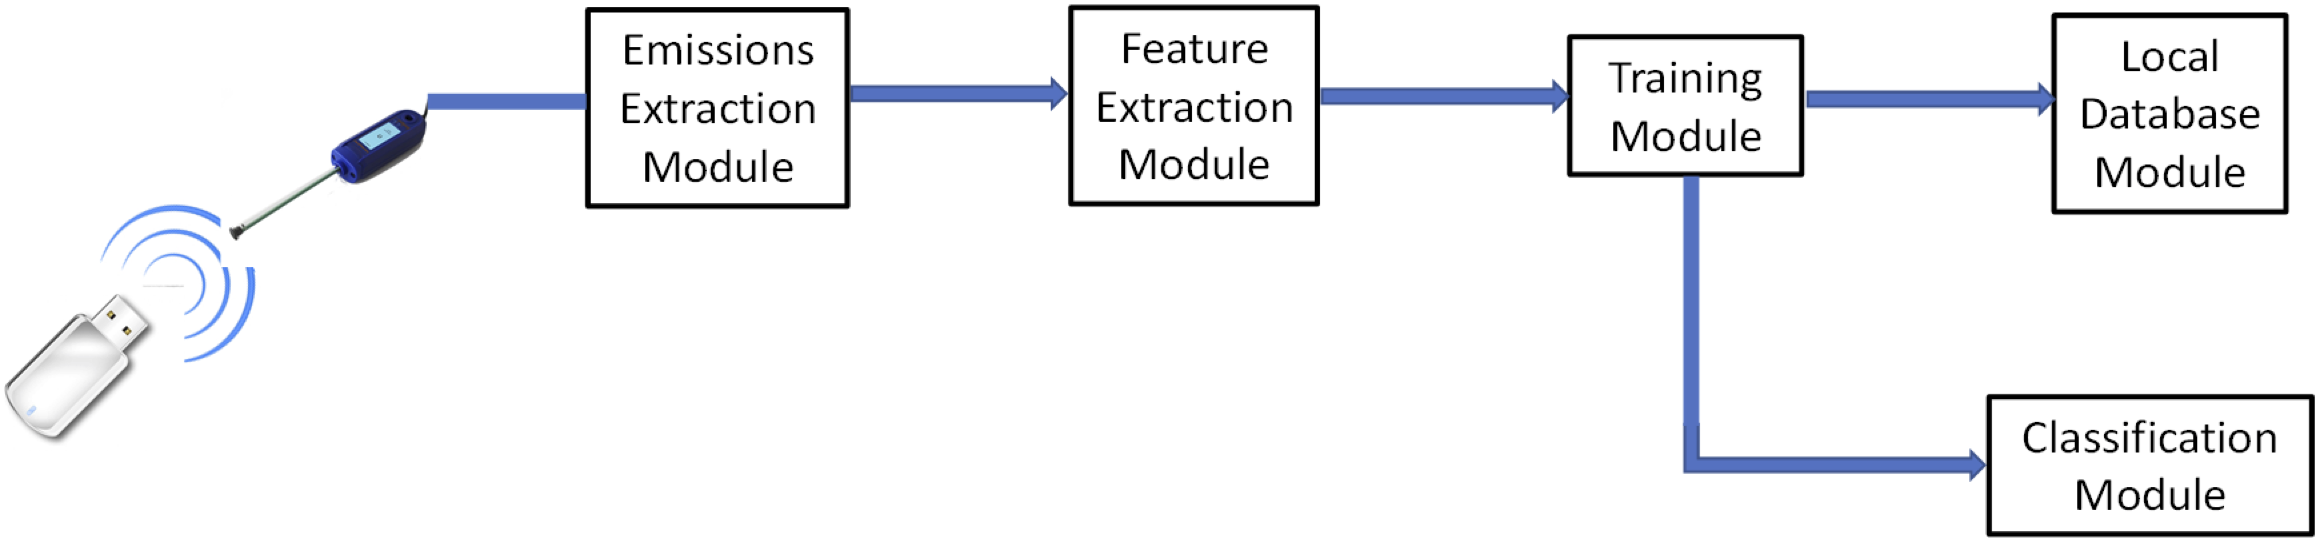
\includegraphics[width=.5\columnwidth]{Figures/system.png}
    \centering
    \caption{Logical architecture of the \sol\ framework.}
    \label{fig:sys}
\end{figure}

We identify two modes of operation:
\begin{itemize}
    \item \emph{Training Mode.} During this phase, a local database is populated with all the profiles of the available USB devices, including the authorized ones.
    \item \emph{Classification Mode.} This is the online operational mode of \sol, where a new unknown USB device is tested to verify if its profile matches the one already collected during the training mode.
\end{itemize}

The details of the modules involved in the \sol\ framework are provided below:

\begin{itemize}
    \item[$\bullet$] \emph{Emissions Extraction Module.} The role of this module is to detect, capture, and log unintentional magnetic emissions from a particular device. Specifically, \sol\ focuses on the analysis of the unintentional magnetic emissions leaked by USB flash drives at boot time, i.e., when the USB device is first connected to the host device and it executes boot operations.  Then, the raw data consisting of: (i) a timestamp; (ii) the acquisition frequency; and, finally, (iii) the value of the \ac{RSS} are passed to the Features Extraction Module. 
    The operations of the Emissions Extraction Module are carried out with particular hardware equipment, able to capture magnetic emissions on the specific operating frequency thanks to a suitable magnetic antenna. More details about the equipment used in our experiments will be provided in Section \ref{sec:experiments}. 
    \item[$\bullet$] \emph{Features Extraction Module}. Starting from the raw data provided by the Emissions Extraction Module, this module is responsible for generating the features of interest for the particular signal. Specifically, this module operates in three different phases, i.e., \emph{Data Normalization}, \emph{Regions Definitions}, and \emph{Features Computation}.
    \begin{itemize}
        \item[-] \emph{Data Normalization}. The data acquired by the Emissions Extraction Module are normalized by re-centering them to the minimum value of the dynamic range of the observation, and then, by re-scaling them by the value of their dynamic range. Specifically, assuming $x_i$ is a sample of the distribution, and $X_{MIN}$ and $X_{MAX}$ are the minimum and the maximum value of the dynamic range, the normalized sample $\hat{x_i}$ is computed as: $\hat{x_i} = \frac{x_i - X_{MIN}}{ \left( X_{MAX} - X_{MIN} \right) } $. 
        
        These operations are crucial to enable cross-comparisons between different measurements, as they contribute to eliminate any small difference in the absolute value of the received power---e.g., due to small misalignment of the measurement setup.
        \item[-] \emph{Regions Definition}. Each value of the \ac{RSS} reported by the \emph{Emissions Extraction Module} is associated with a given timestamp and a specific frequency. In this phase, the \emph{Features Extraction Module} merges in the same observation vector the measurements within a given time and frequency regions, that can be configured uniquely for any specific investigation. The output of this phase is a matrix, containing for each identified region all the collected \ac{RSS} values for the particular experiment.
        \item[-] \emph{Features Computation}. Starting from the matrix created in the previous phase, the \emph{Features Computation} phase is responsible for computing the features on each observation vector.
        
        Assuming now that $X = [x_1, x_2, ..., x_i, ..., x_N]$ is the observation vector containing the normalized intensity of the acquired signal in a given time frame and frequency range, we consider the following statistics: (i) mean; (ii) standard deviation; (iii) variance; (iv) skewness; and, finally, (v) kurtosis, to precisely characterize the unintentional radiated emissions from each USB device. Equations \ref{eq:skewness} and \ref{eq:kurtosis} report the formulas for the skewness and kurtosis, respectively, where $(\bar{X})$ is assumed to be the mean value of the observation vector.
        \begin{equation}
            \label{eq:skewness}
            \gamma =\frac{\tfrac{1}{N} \sum_{i=1}^N (x_i-\bar{X})^3}{\left[\tfrac{1}{N-1} \sum_{i=1}^N (x_i-\bar{X})^2\right]^{3/2}}.
        \end{equation}
        
        \begin{equation}
            \label{eq:kurtosis}
            \kappa = \frac{\sum_{n=1}^N \left( x_i - \bar{X} \right)^4} {\frac{1}{N} \left( \sum_{n=1}^N \left( x_i - \bar{X} \right)^2 \right)^2  }.
        \end{equation}
        
        The output of this phase is a new matrix, containing the value of each feature for the reference experiment.
    \end{itemize}
    
    
    The current matrix containing the values of the features for each time and frequency interval can be passed either to the Training Module or the Classification Module, according to the particular operating mode of \sol.
    \item[$\bullet$] \emph{Training Module.} This module, involved only in the Training Mode, is responsible for creating the reference profile of the particular device under investigation, by using the features previously identified by the \emph{Features Extraction Module}. The created profile is then uploaded to the \emph{Local Database Module}.
    \item[$\bullet$] \emph{Local Database Module.} The local database stores information about the specific training model associated with each device. When a new (previously unknown) device is registered, the \emph{Training Module} establishes the specific statistical model for this device, that is stored in the \emph{Local Database Module}. At the same time, when the \emph{Classification Module} is executed, the \emph{Local Database module} provides the reference statistical models used for comparison and classification. 
    \item[$\bullet$] \emph{Classification Module.} This module, involved only in the Classification Mode, is in charge of establishing if the previously stored profiles match the one extracted from the device under test. The comparison is carried out by considering the specific features considered by the \emph{Features Extraction Module}, and by comparing the obtained features with the stored profiles available in the \emph{Local Database Module}. The module outputs a similarity score, representing how much the magnetic emissions collected from the device under test are similar to the stored profile. If such a score is equal or greater than zero, the device is assumed to be authentic. Otherwise, it is discarded. 
    Among the several possible classifiers available in the literature \cite{Shabtai2009}, in this paper, we have adopted the one-class \ac{SVM} classifier, since it natively fits our objectives. More details will be provided in Section \ref{sec:experiments}.  
    
\end{itemize}

Using the five modules described above, depending on the scenario and the specific objective, either the brand and the model of the USB Flash Drive or the specific USB device can be uniquely characterized when connected to a host device. 

Wrapping up, during the \emph{Training Mode}, the unintentional magnetic emissions leaked by the USB devices are collected via the hardware equipment and the functionalities offered by the \emph{Emissions Extraction Module}. Then, the reference features are extracted from the raw signals by the \emph{Features Extraction Module}, and a reference statistical model is created by the \emph{Training Module} and stored into the \emph{Local Database Module} for future use. 
The process is performed for a large number of devices, to create a database containing an exhaustive number of products of the same device.

During the \emph{classification mode}, all the USB devices are tested, by connecting them to a reference host device and collecting the unintentional magnetic emissions during the boot procedures via the functionalities offered by the \emph{Emissions Extraction Module}. The reference features are computed from the acquired signal, and then passed to the Classification Module, which provides a similarity score, indicating how much the stored profile matches the provided one. 
If no correspondence is found (i.e., the similarity score is negative), the new device is assumed as unauthorized. Instead, if the profile of the unintentional magnetic emissions is found to be consistent with the allowed class (i.e., the score is equal to 0 or positive), the device will be authorized.

It is worth noting that \sol\ focuses on the boot procedures of USB devices, because they are strictly required for the normal operations of the USB themselves. Indeed, being loaded in the firmware, the boot procedures associated with the USB device should not be changed by a non-malicious user. Otherwise,  any modification to the firmware (either intentional or not) will generate significant changes to the magnetic emissions during the boot procedures, indicating therefore that the USB flash drive has been either tampered with or replaced. Such modifications of the behavior of the USB flash drive during the boot operations can be detected by \sol\ and can lead to a timely rejection of the device. More details on the specific modifications that can be done when tampering with USB devices are provided in Section~\ref{sec:discussion}.

\section{Experimental Assessment}
\label{sec:experiments}

In this section, we provide the details of our experimental campaign, aimed at measuring the performance of \sol\ for the classification of either the brand and model of USB flash drives, or the specific USB flash drive, according to the scenarios previously introduced in Section \ref{sec:scenario_adv_model}.
Section \ref{subsec:tools} illustrates the equipment used in our experiments, Section \ref{sec:consistency} provides evidence of the consistency among different observations of boot operations on the same USB flash drives, Section \ref{sec:class_usb} shows the results achieved by \sol\ in the classification of different brand and models of USB flash drives, Section \ref{sec:auth} illustrates how \sol\ achieves the identification of single USB flash drives using more advanced equipment, Section~\ref{sec:exp_fr} provides the accuracy of \sol\ when a reduced number of features is selected, Section~\ref{sec:fw_mod} includes some experiments on firmware modification and, finally, Section~\ref{sec:host_impact} illustrates how the features of the host device impact on the profile of unintentional magnetic emissions radiated by USB flash drives. \\
The code of \sol, including the source data of our experiments and the tools necessary to reproduce our results, are available for download at \cite{crilab}.

\subsection{Tools and Methodology}
\label{subsec:tools}

In our experimental campaign, we used the equipment listed below.
\begin{itemize}
\item \textbf{USB Devices}. We tested the performance of \sol\ with a set of total of 59 different USB devices, related to 17 unique models, whose details are reported in Tab. \ref{tab:usblist}, including the model of the included \emph{Controller Chip}, containing the local oscillator (mainly) responsible for magnetic emissions generation (we notice that the manufacturer SanDisk does not provide any detail about the controller chip).
\begin{table*}[htbp]
\centering
\color{black}
\caption{List of USB Brands and Models adopted in our experiments.}
\begin{tabular}{|l|l|l|}
\hline
\textbf{Device} & \textbf{Controller Chip} & \textbf{Device ID} \\ \hline
HPx900w-64GB \cite{HP}& PHISON-PS2251-09-V & U1 \\ \hline 
JUANWE-32GB \cite{JU} & FirstChip-FC1179 & U2 \\ \hline
 Kingston Digital 16GB Data Traveler G4 \cite{KD} & PHISON-PS2251-09-V & U3 \\ \hline
Mosdart-8GB \cite{MD} & AlcorMP & U4 \\ \hline
PNY Turbo 128GB \cite{PNY} & PHISON-PS2251-09 & U5 \\ \hline
Patriot 128GB Supersonic Rage Series \cite{PR} & PHISON-PS2251-09-V & U6 \\ \hline
Rubber Ducky \cite{RubberDucky} & Atmel 32UC3B1 & U7 \\ \hline
Samsung BAR Plus 32GB \cite{SB} & Silicon Motion SM3267 & U8 \\ \hline
SanDisk Ultra 128GB \cite{SU}& SanDisk & U9 \\ \hline
SanDisk Cruzer 128GB \cite{S128} & SanDisk & U10 \\ \hline
SanDisk Cruzer 32GB \cite{S32} & SanDisk & U11 \\ \hline
SanDisk Cruzer 64GB \cite{SD} & SanDisk & U12 \\ \hline
Silicon Power 32 GB Blaze B30 \cite{SP} & PHISON-PS2251-09-26 & U13 \\ \hline
Toshiba TransMemory 64GB \cite{TO} & PHISON-PS2251-11 & U14 \\ \hline
SanDisk 16 GB \cite{S16GB} & SanDisk  & U15 \\ \hline
Strontium 16 GB \cite{StrontiumUSB} & Strontium  & U16 \\ \hline
Klevv Neo C20 16GB \cite{KlevvNeo} & Essencore & U17 \\ \hline

\end{tabular}
\label{tab:usblist}
\end{table*}
We selected these brands to create a large dataset, considering both the most used models and any possible factor affecting the magnetic emissions of such devices. Specifically, SanDisk, Samsung, and Kingston USB flash drives are the top three brands purchased by users on Amazon---as of July 2019 \cite{AmazonList}. At the same time, Juanwe, PNY, HP, and Mosdart are all positioned among the top 10 brands. 
In addition, we also selected some brands based on the use of the same version of the micro-controller. For instance, we highlight that the micro-controller of the HP (U1), the Kingston (U3), the PNY (U5), the Patriot (U6), the Silicon Power (U13), and the Toshiba (U14) are the same, i.e., they feature the same hardware chip, while the layout of the \ac{PCB} and/or the versions of the firmware are different (e.g., 09-V for the Kingston, 09-26 for the Silicon Power) \cite{phison}. Also, it is also worth noticing that we considered different devices having the same brand, model, and firmware: specifically, we considered $15$ \emph{SanDisk 16GB}, $15$ \emph{Strontium 16GB} and $15$ \emph{Klevv Neo C20 16GB}.
%we considered 5 \emph{Mosdart}, 3 \emph{SandiskCruzer64GB}, 2 \emph{Juanwe}, 2 \emph{Samsung BAR}, and 2 \emph{SanDiskCruzer32GB} USB Flash Drives.
All the devices have been analyzed as provided by the manufacturer, without any modification to the legacy firmware. To prove the effectiveness of our method, we acquired the magnetic emissions by temporarily removing the case of the USB flash drive. %Indeed, the results provided in Section~\ref{sec:class_usb} indicate that the modifications introduced by the case are unique, thus still allowing for the correct identification of the brand and model of the USB flash drive. 
Besides, we highlight the presence of a \emph{malicious} device, i.e., a USB Rubber Ducky. This USB Flash drive is a cross-platform keystroke injection tool, able to work effectively with either Windows, Mac, or Linux. It features a 60 MHz 32-bit processor, hidden in the form factor of an ordinary generic USB flash drive. It consists mainly of a CPU chip and a micro SD storage, used to upload malicious payloads to the host device. 
Once connected to a host machine, the Rubber Ducky is recognized as a keyboard. Thus, the host device accepts its payload, consisting of pre-programmed regular keyboard strokes, up to a maximum rate of 1000 words per minute \cite{RubberDucky}. The commands are programmed using a dedicated scripting language, and it is possible to perform a wide range of automated functions, such as password brute-forcing, binaries injection, shell reversing, as well as changing system settings. Nowadays, it is mainly used by professionals, penetration testers, and system administrators.
    
\item \textbf{Aaronia PBS2 EMC Probe set}. To collect the unintentional magnetic emissions radiated by the USB devices, we used the Aaronia PBS2 EMC Probe set \cite{PBS2}. This equipment allows straightforward pinpointing and measurement of interference in the frequency band from the DC (1Hz) up to 9GHz in electronic component groups, as well as the execution and monitoring of generic Electro-Magnetic measurement. 
As a probe, we used a 25mm magnetic (H) field probe PBS-H3, covered with an insulating layer, thus providing a safe measurement environment for oscillators and mains lines. This probe is connected to the UBBV2 40dB EMC RF pre-amplifier, allowing for a clear separation between the useful signal and the surrounding noise. The probe is then connected via a low-impedance cable to a \ac{SDR}.
    
\item \textbf{HackRFOne \acl{SDR}}. The HackRFOne \ac{SDR} has been used to record unintentional magnetic emissions acquired from the Probe Set over a frequency span of 10 MHz, and to convert raw data (in the form of regular I-Q samples) into spectral power density measurements. Specifically, the SDR performs a \ac{FFT} on the provided I-Q data and it generates, for each time frame, a tuple containing a reference timestamp (in milliseconds), a frequency (in Hz), and a power level (in dBm). Tab. \ref{tab:hackrf_conf} provides the details of the configuration of the \ac{SDR}.
\begin{table}[htbp]
\centering
\caption{Configuration of the HackRFOne Software Defined Radio.}
\begin{tabular}{|P{4.8cm}|P{2.8cm}|}
    \hline
    \textbf{Feature} & \textbf{Value} \\ \hline
        \text{Resolution Bandwidth} & 976.6 Hz \\ \hline
    \text{Center Frequency} & 5 MHz \\ \hline
    \text{Start Frequency} & 0 MHz \\ \hline
    \text{Stop Frequency} & 10 MHz \\ \hline
    %\text{Frequency Span} & 10 MHz \\ \hline
    \text{Reference Level} & -5 dB \\ \hline
    \text{FFT Size} & 8192 samples \\ \hline
\end{tabular}
\label{tab:hackrf_conf}
\end{table}
    
\item \textbf{Rohde \& Schwarz FSW8 Spectrum Analyzer}. The Rohde \& Schwarz FSW8 Spectrum Analyzer has been used in place of the HackRFOne to record unintentional magnetic emissions acquired from the Probe Set over a larger frequency span, up to 200 MHz. As with the HackRFOne, the equipment automatically converts raw data into spectral power density measurements, by performing the \ac{FFT} over the acquired samples, and it provides a tuple for each time frame, containing a timestamp (in milliseconds), a frequency (in Hz), and a power level (in dBm). Table~\ref{tab:SAconf} provides the details of the configuration of the spectrum analyzer.
    
\begin{table}[htbp]
    \centering
    \caption{Configuration of the Rohde \& Schwarz FSW8 Spectrum Analyzer.}
    \label{tab:SAconf}
    \begin{tabular}{|P{4.8cm}|P{2.8cm}|}
    \hline
    \textbf{Feature} & \textbf{Value} \\ \hline
    Video Bandwidth & 3 MHz \\ \hline
    Resolution Bandwidth & 3 MHz \\ \hline
    Center Frequency & 100 MHz \\ \hline
    Start Frequency & 0 MHz \\ \hline
    Stop Frequency & 200 MHz \\ \hline
    Frequency Span & 200 MHz \\ \hline
    RF Attenuation & 10 dB \\ \hline
    Reference Level & -5 dB \\ \hline
    Sweep time & 4.01 ms \\ \hline
    Sweep points & 4001 \\ \hline
    \end{tabular}
\end{table}

\item \textbf{Matlab R2020a}. Matlab R2020a has been used to implement the \emph{Features Extraction Module}, the \emph{Training Module}, the \emph{Local Database Module}, and the \emph{Classifier Module}. As the classification algorithm, we used the one-class \ac{SVM} classifier provided by the Machine Learning Toolbox of Matlab. Specifically, the one-class SVM classifier analyzes each of the USBs as a standalone USB flash drive, by creating a profile that matches the features provided for the particular USB brand (or the specific USB flash drive). When a test set is provided in input for classification, as an output, the one-class SVM classifier provides an \emph{evaluation score} for each input sample. Such evaluation score indicates the likelihood that the specific input sample is consistent with the created model, or not. This approach is particularly useful when the range of possible classes is wide, such as for USB flash drives, and thus a multi-class classification approach is not suitable.
\end{itemize}

All the experiments described in the following subsection have been conducted by collecting the unintentional magnetic emissions radiated by the target USB devices in regular laboratory conditions, without any effort to reduce the environmental noise. Our measurement setup is shown in Figure \ref{fig:setup}. 
\begin{figure}[htbp]
    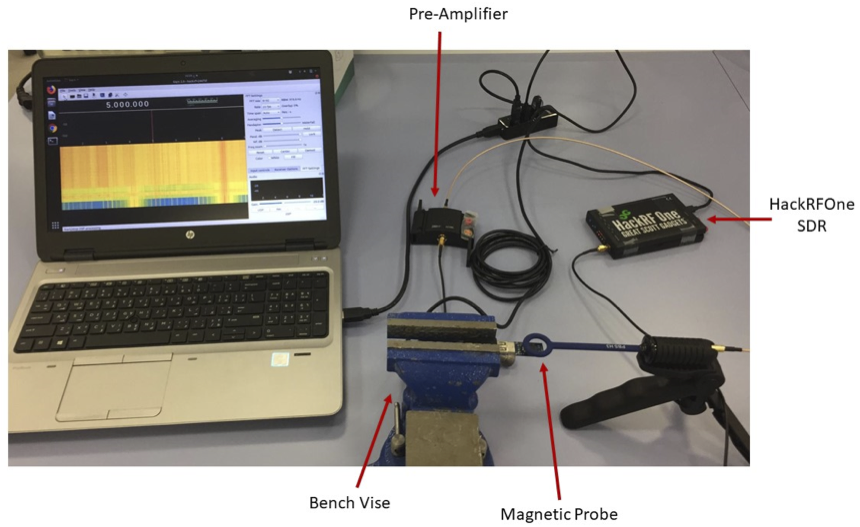
\includegraphics[width=.5\columnwidth]{Figures/setup_labels.png}
    \centering
    \caption{Measurements Setup.}
    \label{fig:setup}
\end{figure}

Note that a USB cable extension was placed on a Bench Vise, to physically stabilize the USB device under test. In addition, this setup allows having uniform conditions for emissions collection. The Magnetic Probe has been placed on top of the USB device controller chip, in a way to clearly capture the radiated emissions. 
For each USB device under test, ten different boot sequences were acquired, where each measurement was at least 3.35 seconds long.

Finally, for the data processing, we used a Lenovo Ideapad 320 laptop, equipped with an Intel i7-7500 processor running at 2.70 GHz and equipped with 8 GB of RAM.

\subsection{Consistency of Unintentional Magnetic Emissions Radiated from USB Devices}
\label{sec:consistency}

Our first investigation aims at establishing the feasibility of uniquely identifying either the brand and model of the USB flash drive or the specific USB device, based on the profile of the unintentional magnetic emissions.

Figure \ref{fig:RD} shows two sample measurements acquired at different times, related to the unintentional magnetic emissions radiated from the same Rubber Ducky USB flash drive (U7), during the boot procedures. Because of the normalization phase occurring in the \emph{Features Extraction module}, all the samples corresponding to given times and frequencies have a value between 0 and 1. Specifically, the blue color maps values in the range $\left[ 0 - 0.25 \right[$, the cyan corresponds to values in the range $\left[ 0.25 - 0.5 \right[$, the yellow is related to values in the range $\left[ 0.5 - 0.75 \right[$, while the red color indicates value in the range $\left[ 0.75 - 1 \right]$.
\begin{figure}[htbp]
    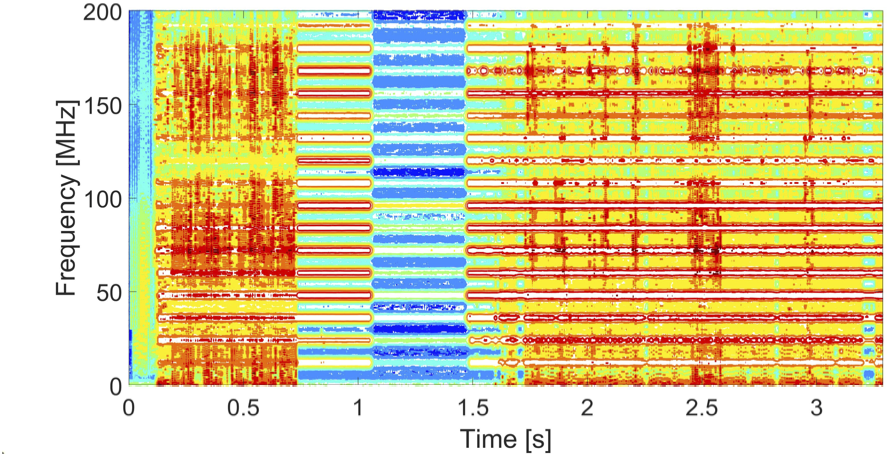
\includegraphics[width=.49\columnwidth]{Figures/RD_1.png}
    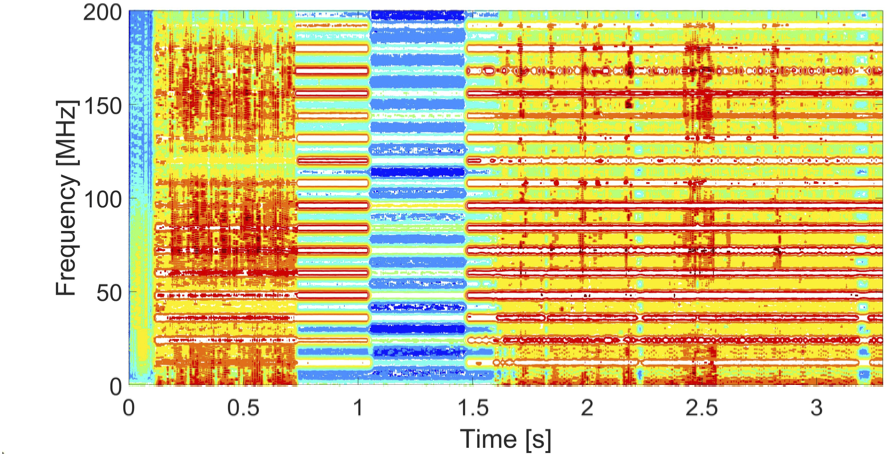
\includegraphics[width=.49\columnwidth]{Figures/RD_2.png}
    \centering
    \caption{Profile of the unintentional magnetic emissions of a Rubber Ducky USB flash drive (U7), during two different executions of the boot procedures.}
    \label{fig:RD}
\end{figure}

First, we notice that the time duration of our experiments is enough to capture not only the boot phase, where the whole system is powered up and initialized, but also to acquire the following idle state, where the USB device waits for instructions by the target USB device.

By comparing the two figures, it emerges that different recordings have similar normalized power profiles, as per the time and the frequency. Indeed, small differences can be found in the time domain, due to a different delay between the time instant at which the acquisition was started and the time instant where the USB device was connected to the host device, and in the intensity of the unintentional radiation emissions, due to the surrounding noise and minimal displacement between the USB device and the probe. However, even across different measurements, different acquisitions of the unintentional radiated emissions from the same USB device are consistent, confirming that their statistical analysis can be effectively used for discriminating the USB brand and model. 

% \textcolor{black}{
% Similarly, the profile of unintentional magnetic emissions from two different USB Flash Drives characterized by the same brand and model appears very similar. Figure~\ref{fig:mosdart} reports an example for two Mosdart USB Flash Drives (U4), over the frequency span of 200~MHz.
% \begin{figure}[htbp]
%     \includegraphics[width=.6\columnwidth]{Figures/mosdart1.eps}
%     \includegraphics[width=.6\columnwidth]{Figures/mosdart2.eps}
%     \centering
%     \caption{Profile of the unintentional magnetic emissions of two different Mosdart USB Flash Drives (U4), during the execution of the boot procedures.}
%     \label{fig:mosdart}
% \end{figure}
% % % Different USB Flash Drives
% Finally, we notice that comparing two different USB flash drives (e.g., Figure 3 and Figure 4), the profiles are very different. Thus, their features can be used to recognize the brand and model of the specific USB Flash Drive.
% }

\subsection{Scenario \#1: Classification of USB flash drives brand and model}
\label{sec:class_usb}

The \emph{Scenario \#1} described in Section \ref{sec:scenario_adv_model} involves the identification of the brand and model of the specific USB Flash Drive under test. As shown in the previous section, different brands of USB Flash Drives are characterized by a very different profile of magnetic emissions. This motivates the use of relatively cheap equipment, i.e., the HackRFOne \ac{SDR}, as the tool for data acquisition and processing. We recall that the HackRFOne has a maximum acquisition bandwidth of 10 MHz. Thus, this frequency span can be used only to classify USB flash drives brands and models.

To enable cross-comparisons, we considered a fixed observation window of 1.08 seconds for each of the acquired traces. This time-slot was further divided into a given number of time and frequency regions, leading to a specific number of features characterizing each observation.

To provide sufficient robustness to the classification, we considered a total number of $325$ features, computed as follows. We first considered the overall observation interval of 1.08 seconds, and we computed (5) features, i.e., the mean, standard deviation, variance, skewness, and kurtosis of the samples in the whole interval (see Section~\ref{sec:idea} for the details of the computation of each feature). This step results in a total of 5 features. Then, we further divided the overall observation interval of 1.08 seconds in four (4) time regions, each region lasting $0.27$~s. For each time region, we computed the same five (5) features listed above. This step results in a total of 20 features. Then, we further divided each of the four (4) time regions into fifteen (15) frequency regions, where each frequency region has a bandwidth of $666.67$~Hz. For each of the $15 \cdot 4$ regions, we computed the same five (5) features listed above. This step results in a total $15 \cdot 4 \cdot 5 = 300$ features. Summing up the three steps, we have a total of $5 + 20 + 300 = 325$ features.

Specifically, the detection of authorized devices against not-authorized ones has been performed resorting to the one-class SVM classifier (see Section~\ref{sec:idea} for more details). For the Scenario \# 1, we considered 17 different models of USB Flash Drives (classes), i.e., \{$U1, \ldots, U17$\}, and we performed $10$ observations (measurements) for each class, for a total of $170$ observations. Moreover, we adopted the 10-fold cross-validation where, in each fold, $90\%$ of the observations (from each class) have been selected for the training process. Then, we test the remaining observations ($10\%$) against the models created for each USB flash drive (disjoint from the test set and therefore not containing any testing sample), and we evaluate the accuracy of the model through a \emph{similarity score}. Note that we have $17$ \emph{similarity scores} for each testing sample, i.e., the score resulting from the evaluation of the testing sample against each of the $17$ classes (USB flash drives). Therefore, this strategy leads to a set of $17$ similarity scores for each testing sample, and a total number of $17 \cdot 170 = 2,890$ \emph{similarity scores}.

Figure~\ref{fig:classification_scenario1} shows the computed similarity scores as a function of the 17 considered classes \{$U1, \ldots, U17$\}. For each class (USB device), we reported as green circles ($10$ samples per class) the observations coming from the authorized device, while we considered the black dots ($160$ samples) for the non-authorized ones. 

\begin{figure}[htbp]
    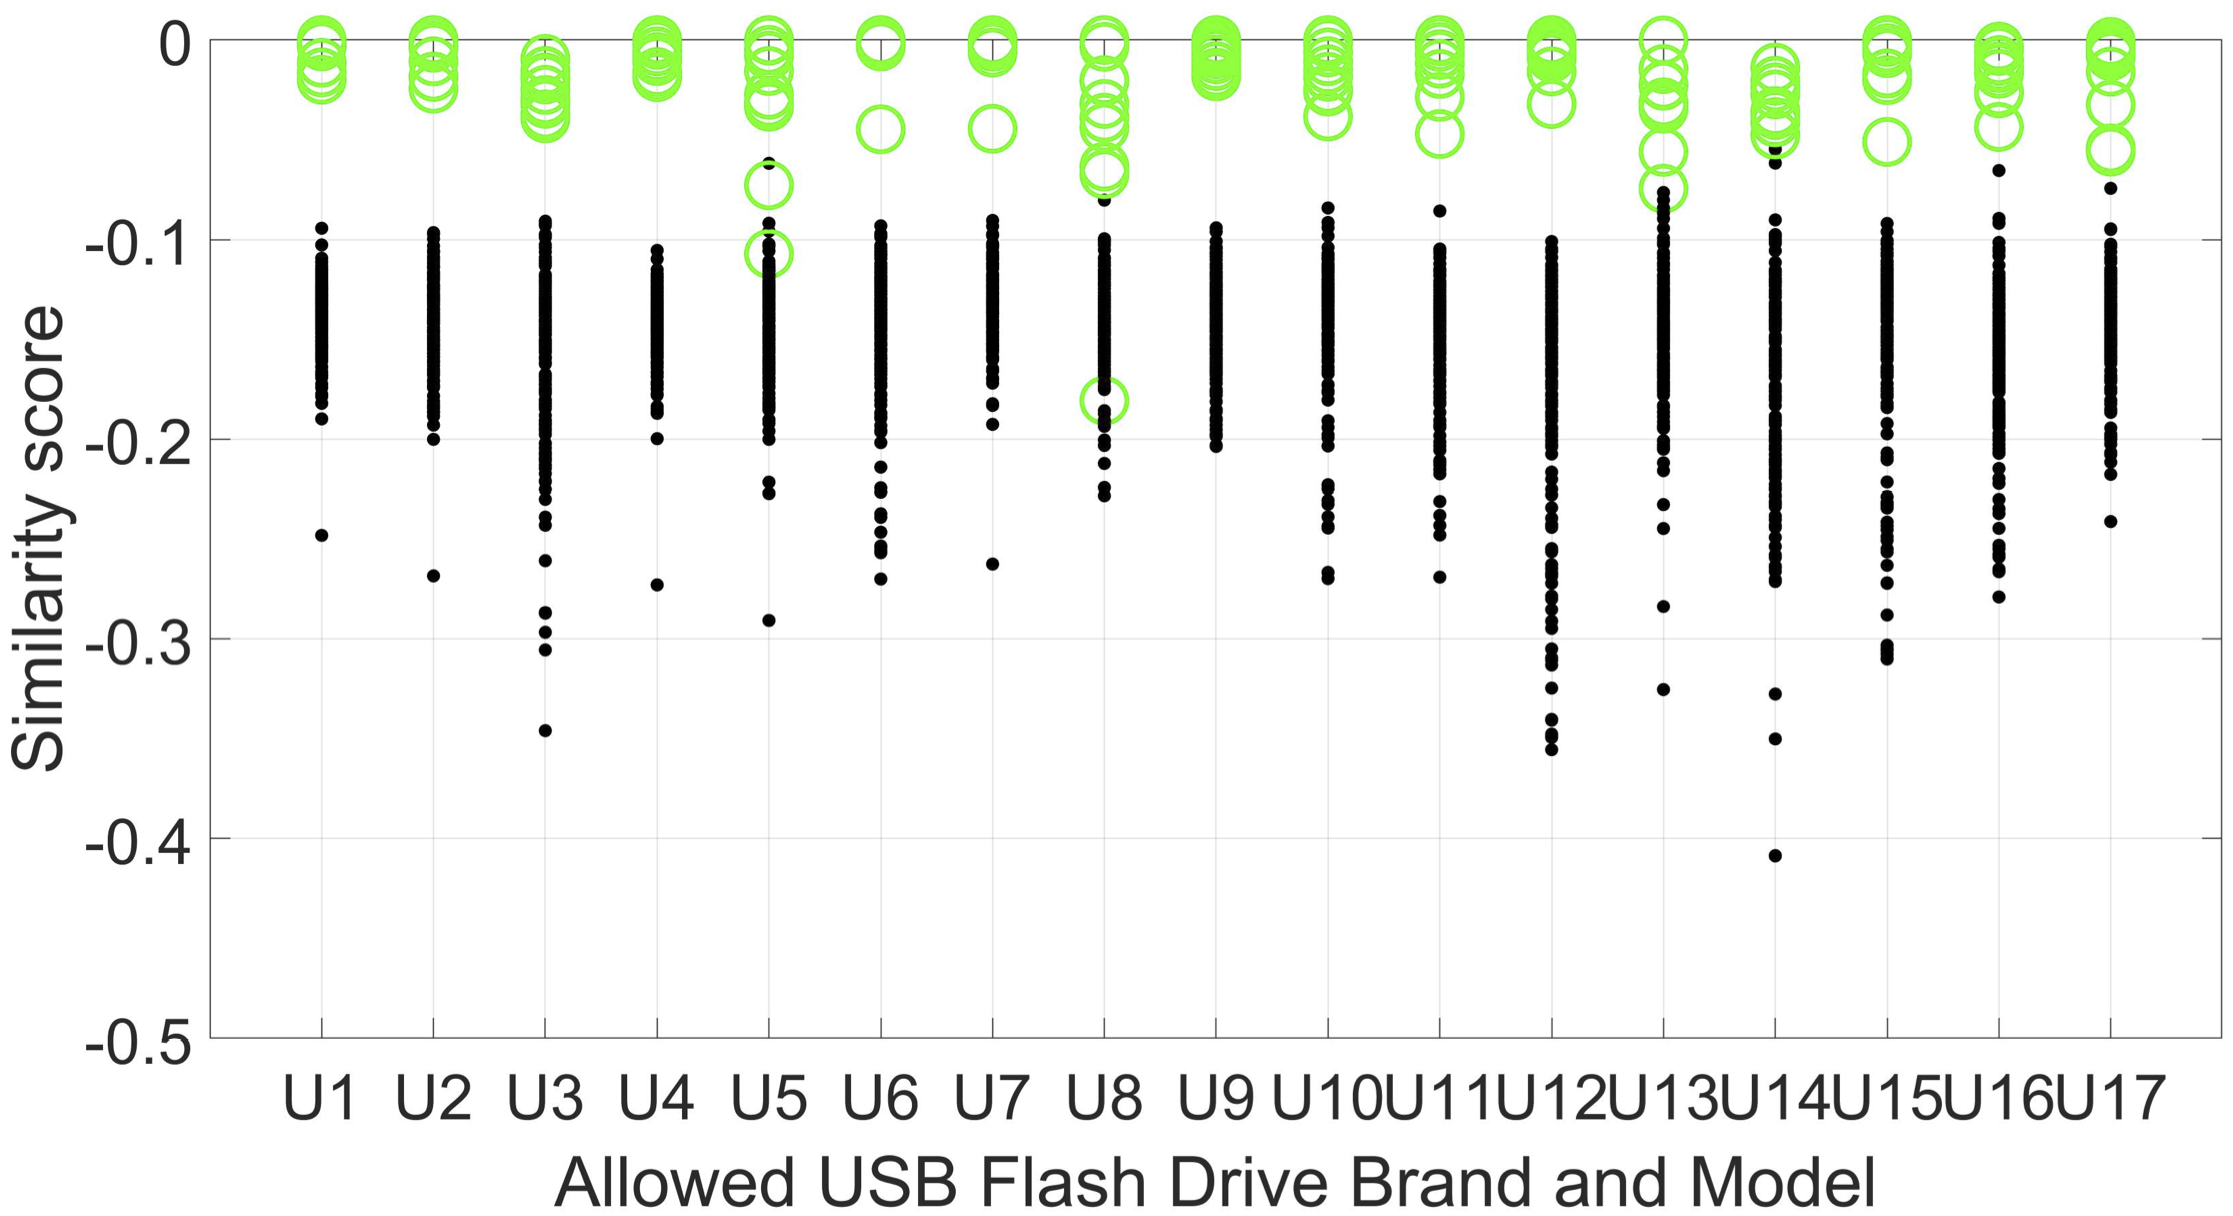
\includegraphics[width=.6\columnwidth]{Figures/scenario1_svm_final.png}
    \centering
    \caption{Classification performance of \sol. Each column refers to a set of $170$ experiments where just one USB flash drive model is assumed to be authorized. Green circles report the value of the similarity score of the classifier for the authorized device, while black dots report similarity score for the unauthorized USB brands.}
    \label{fig:classification_scenario1}
\end{figure}

It is worth noting that, in the vast majority of the experiments, the authorized USB flash drives report values that are very close to $0$ and less than the value of $-0.01$, while the unauthorized ones report lower scores. Overall, given that the model of each USB flash drive is trained and validated on its own, we should select a threshold value for each USB brand, and decide to \emph{accept} it as authorized if the evaluation score is higher than the threshold. As a worst-case, we notice that selecting a general threshold $T=-0.075$ guarantees \ac{TPR} $0.982$ (i.e., $98$\% of the authorized brands are correctly recognized), and a \ac{FPR} of only $0.001$ (i.e., only $0.01$\% of the unauthorized brands are erroneously recognized as authorized). However, a threshold can be selected for each USB flash drive. For instance, focusing on the USB Flash Drive $U7$, the threshold value $T_7 = -0.0365$ provides TPR $1$ and FPR $0$, i.e., the best possible result.\\
We remark that the above results show that \sol\ can distinguish the brand and the model of the USB flash drive, even if the brands share the same controller chip version and same PCB layout. For instance, we can distinguish the specific USB flash drive model among the HPx900w-64GB, the Kingston Digital 16GB Data Traveler G4, and the Patriot 128GB Supersonic Rage Series, despite these three models share the same controller chip and PCB layout, i.e., the PHISON-PS2251-09-V.\\
The above results suggested that, to some extent, \sol\ can identify not only the specific hardware chip but also the code that is executed during the boot. 
Indeed, \sol\ can discriminate also between the HP, Kingston, PNY, Patriot, Silicon Power, and Toshiba USB flash drives, even if they are based on the same hardware chip. Indeed, we recall that their PCB and/or the version of the firmware is different, and this leads to a different profile in the unintentional magnetic emissions at lower frequencies during the boot operations. More details on the impact of the firmware running on a particular chip will be provided in Section~\ref{sec:fw_mod}.

We also investigated the time required by \sol\ to provide the decision. Using 325 features, over a set of $2,890$ experiments, \sol\ requires $11.5$~ms on average, with a lower confidence interval of $10.27$~ms and higher confidence interval of $12.72$~ms.

Finally, we notice that, in principle, any Machine-Learning (ML) and Deep Learning (DL) classification tool can be used to precisely classify the magnetic emissions radiated by the tested USB Flash Drives. However, we highlight that the scope of our paper is not to find the best classification tool for this problem, but to show that unintentional magnetic emissions can be used to fingerprint the brand and the model of commodity USB Flash Drives. The data acquired from the tested USB Flash Drives have been released as open-source, to give to interested researchers the opportunity to test additional ML or DL classification tools and further boost the performance of \sol \cite{crilab}.

\subsection{Scenario 2: Identifying the specific USB Flash Drive}
\label{sec:auth}

In the context of the \emph{Scenario \#2}, it is of crucial importance to uniquely identify the specific USB flash drive, to protect the Critical Infrastructure against malicious software injection. As shown in Section \ref{sec:consistency}, identifying uniquely a USB Flash Drive involves discriminating very subtle differences in the profile of the unintentional magnetic emissions, possibly spanning a wide spectrum. To this aim, more powerful equipment should be used, characterized by a wider real-time bandwidth resolution, such as the \emph{Rohde \& Schwarz FSW8} Spectrum Analyzer, leading to an increased number of features, that could be processed by a more powerful processing unit.

To investigate the feasibility of this setup of \sol\ to uniquely identify USB Flash Drives, we considered USB Flash Drives of the same brand and model, and we applied \sol\ to identify them uniquely. 
We considered a fixed observation window of 3.35 seconds for each of the acquired traces, and the same number of features ($325$), derived as previously explained.
Note that the methodology to test the performance of \sol\ is still the same previously described: in each experiment, we assumed a selected USB Flash Drive to be the allowed one, while the others were assumed to be rejected, and we used the 10-fold cross-validation, where in each fold, 90\% of the recordings were used in the \emph{Training Mode}, and the remaining 10\% were used to test the \emph{Classification Mode}.

We considered three different USB Flash Drive brands: the SanDisk 16GB (U15), the Strontium 16GB (U16), and the Klevv Neo C20 16GB (U17), where $15$ USB flash drives were available for each experimentation. The results are reported in Figures \ref{fig:scenario2_sandisk},~\ref{fig:scenario2_strontium} and \ref{fig:scenario2_klevv} for the SanDisk, the Strontium and the Klevv Neo C20, respectively. Note that, now, each column contains $15 \cdot 10 = 150$ experiments, where $10$ experiments refer to the authorized USB flash drive and $140$ experiments refer to the unauthorized drives. \\
\begin{figure}[htbp]
    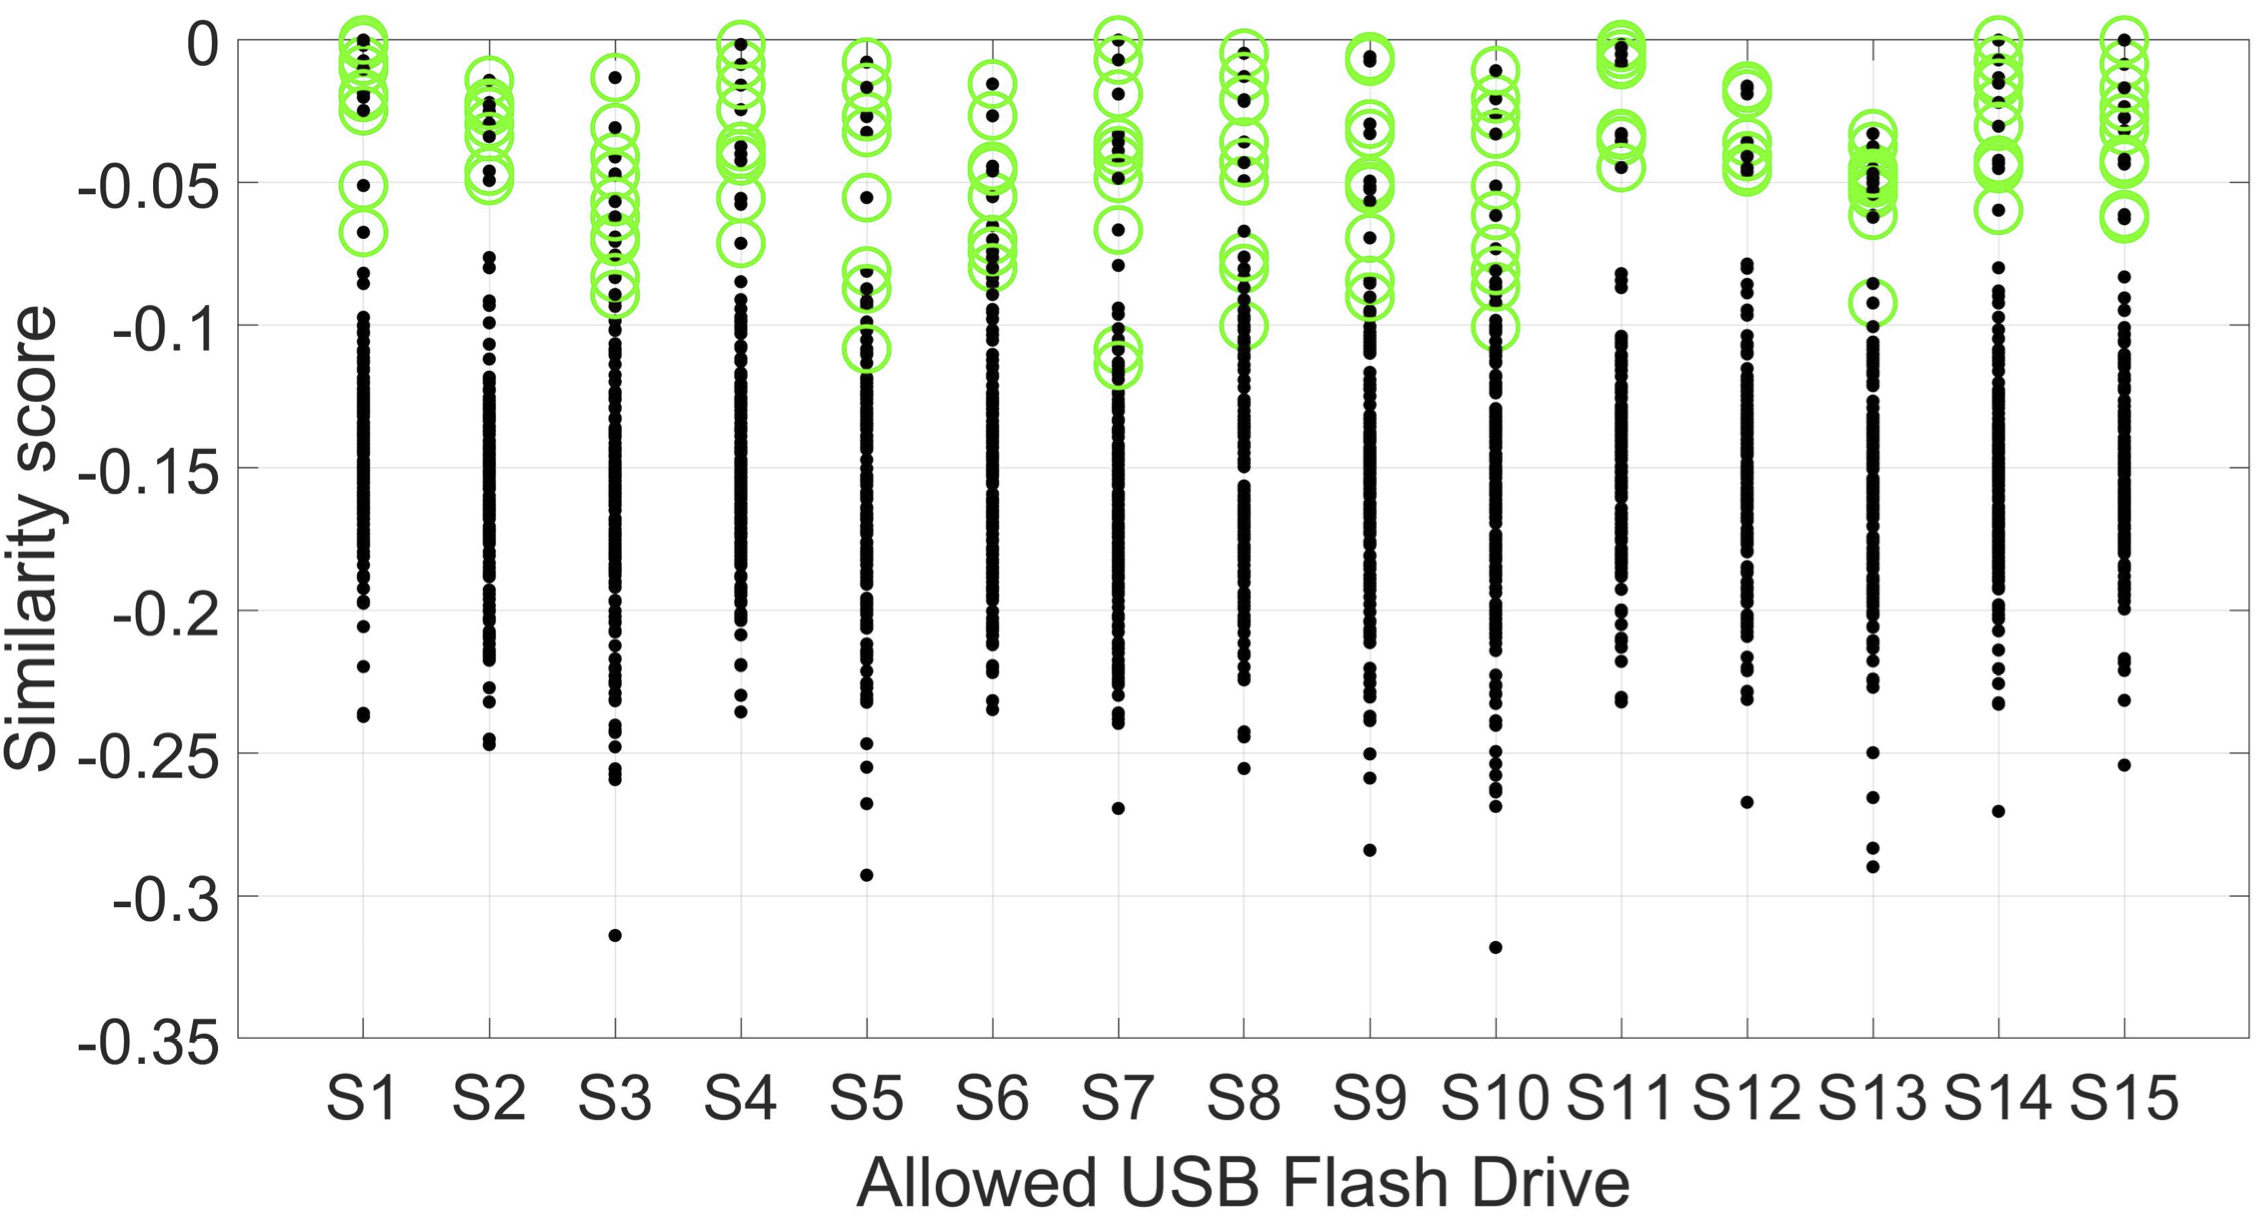
\includegraphics[width=.6\columnwidth]{Figures/scenario2_sandisk_final.png}
    \centering
    \caption{Classification accuracy of \sol\ considering 15 SanDisk 16GB USB Flash Drives.}
    \label{fig:scenario2_sandisk}
\end{figure}
\begin{figure}[htbp]
    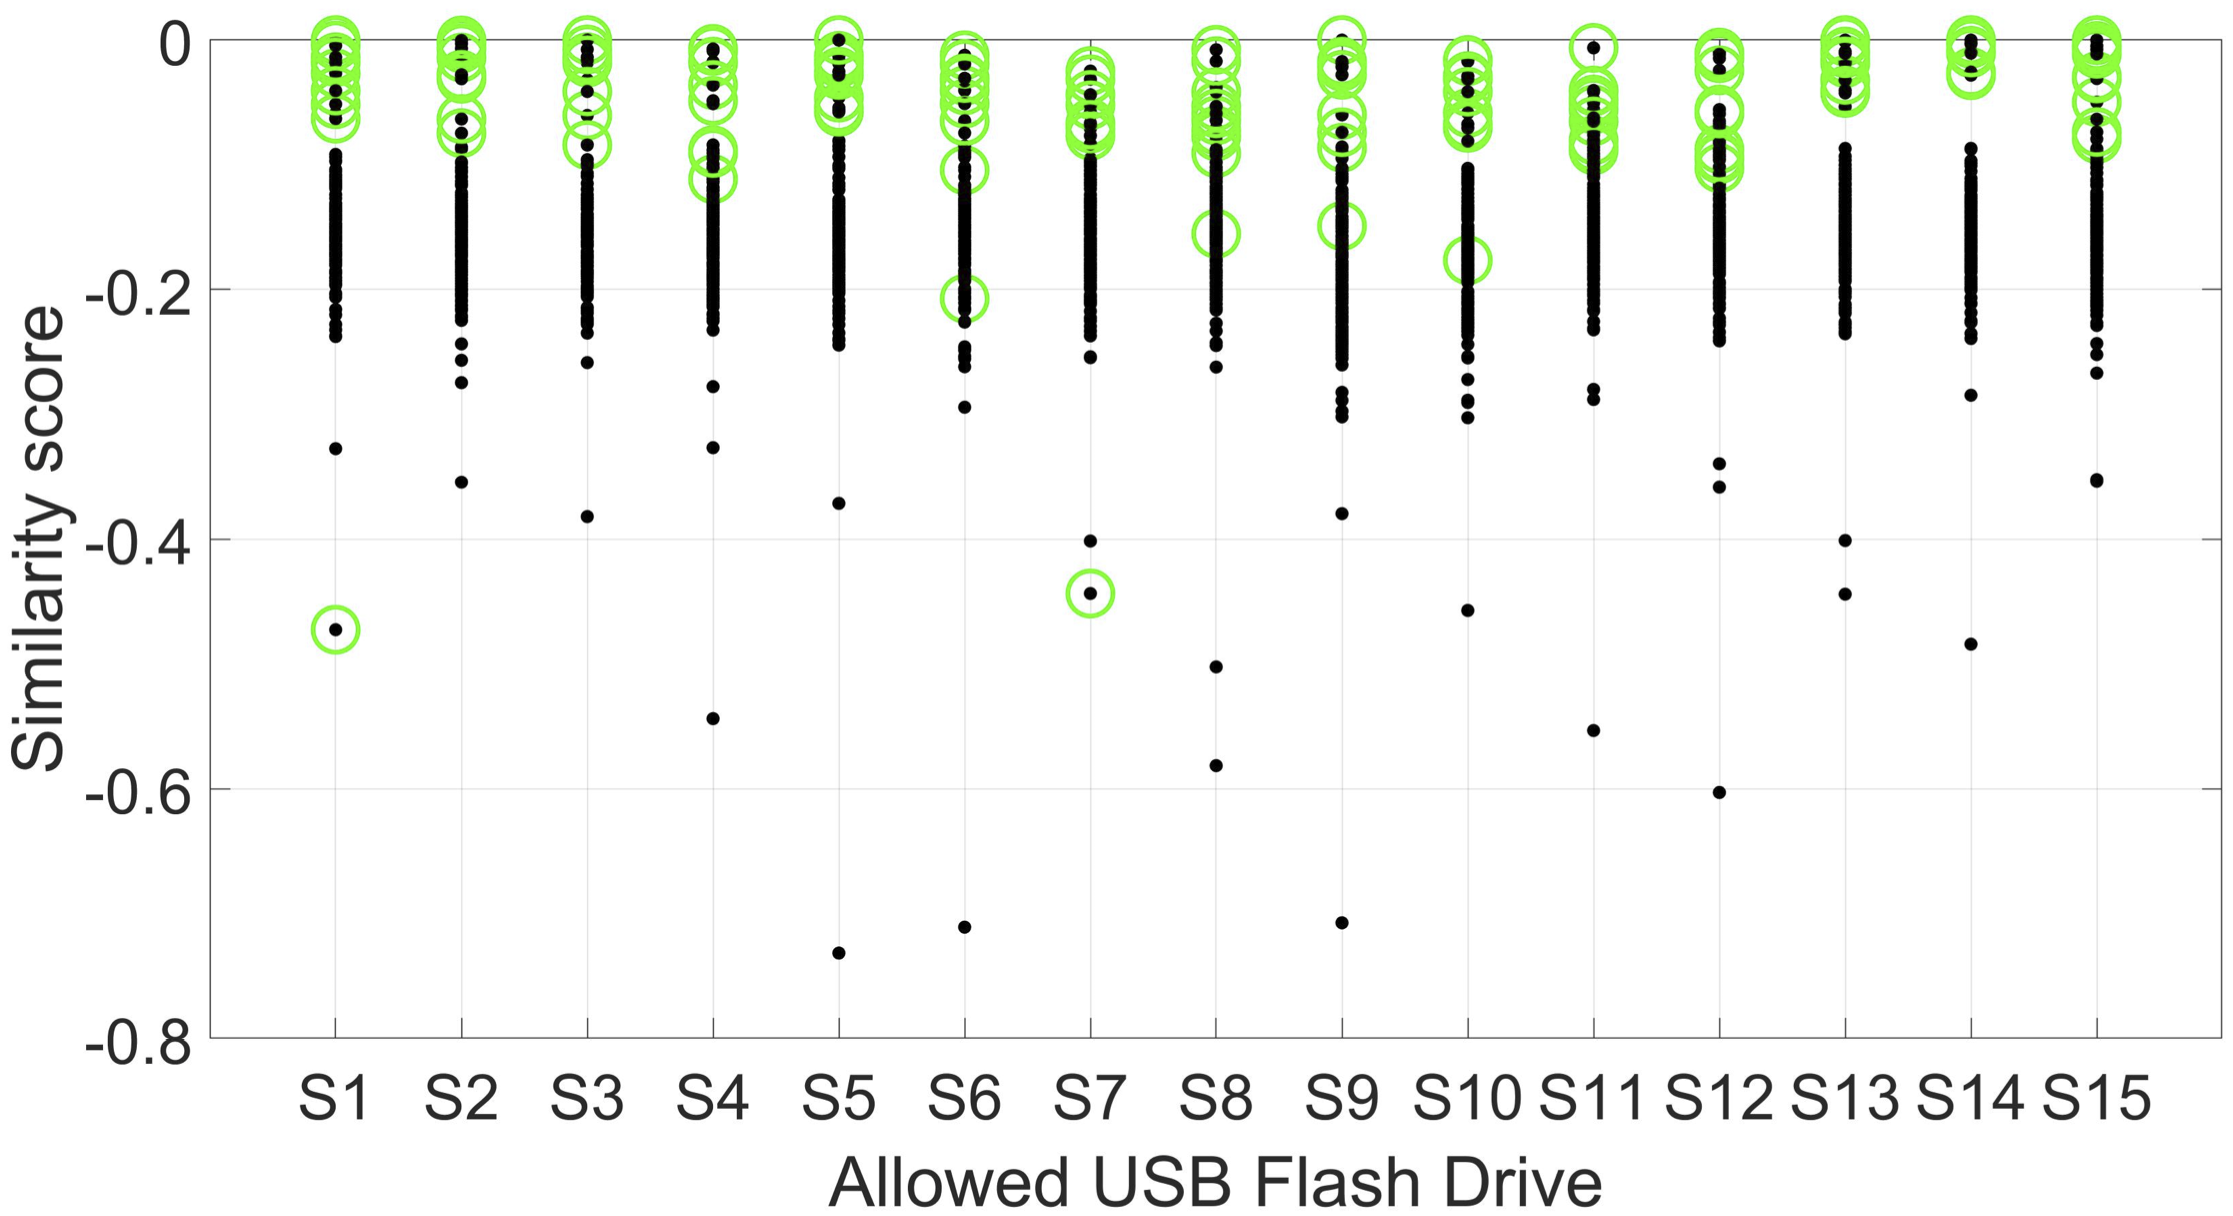
\includegraphics[width=.6\columnwidth]{Figures/scenario2_strontium_final.png}
    \centering
    \caption{Classification accuracy of \sol\ considering 15 Strontium 16GB USB Flash Drives.}
    \label{fig:scenario2_strontium}
\end{figure}
\begin{figure}[htbp]
    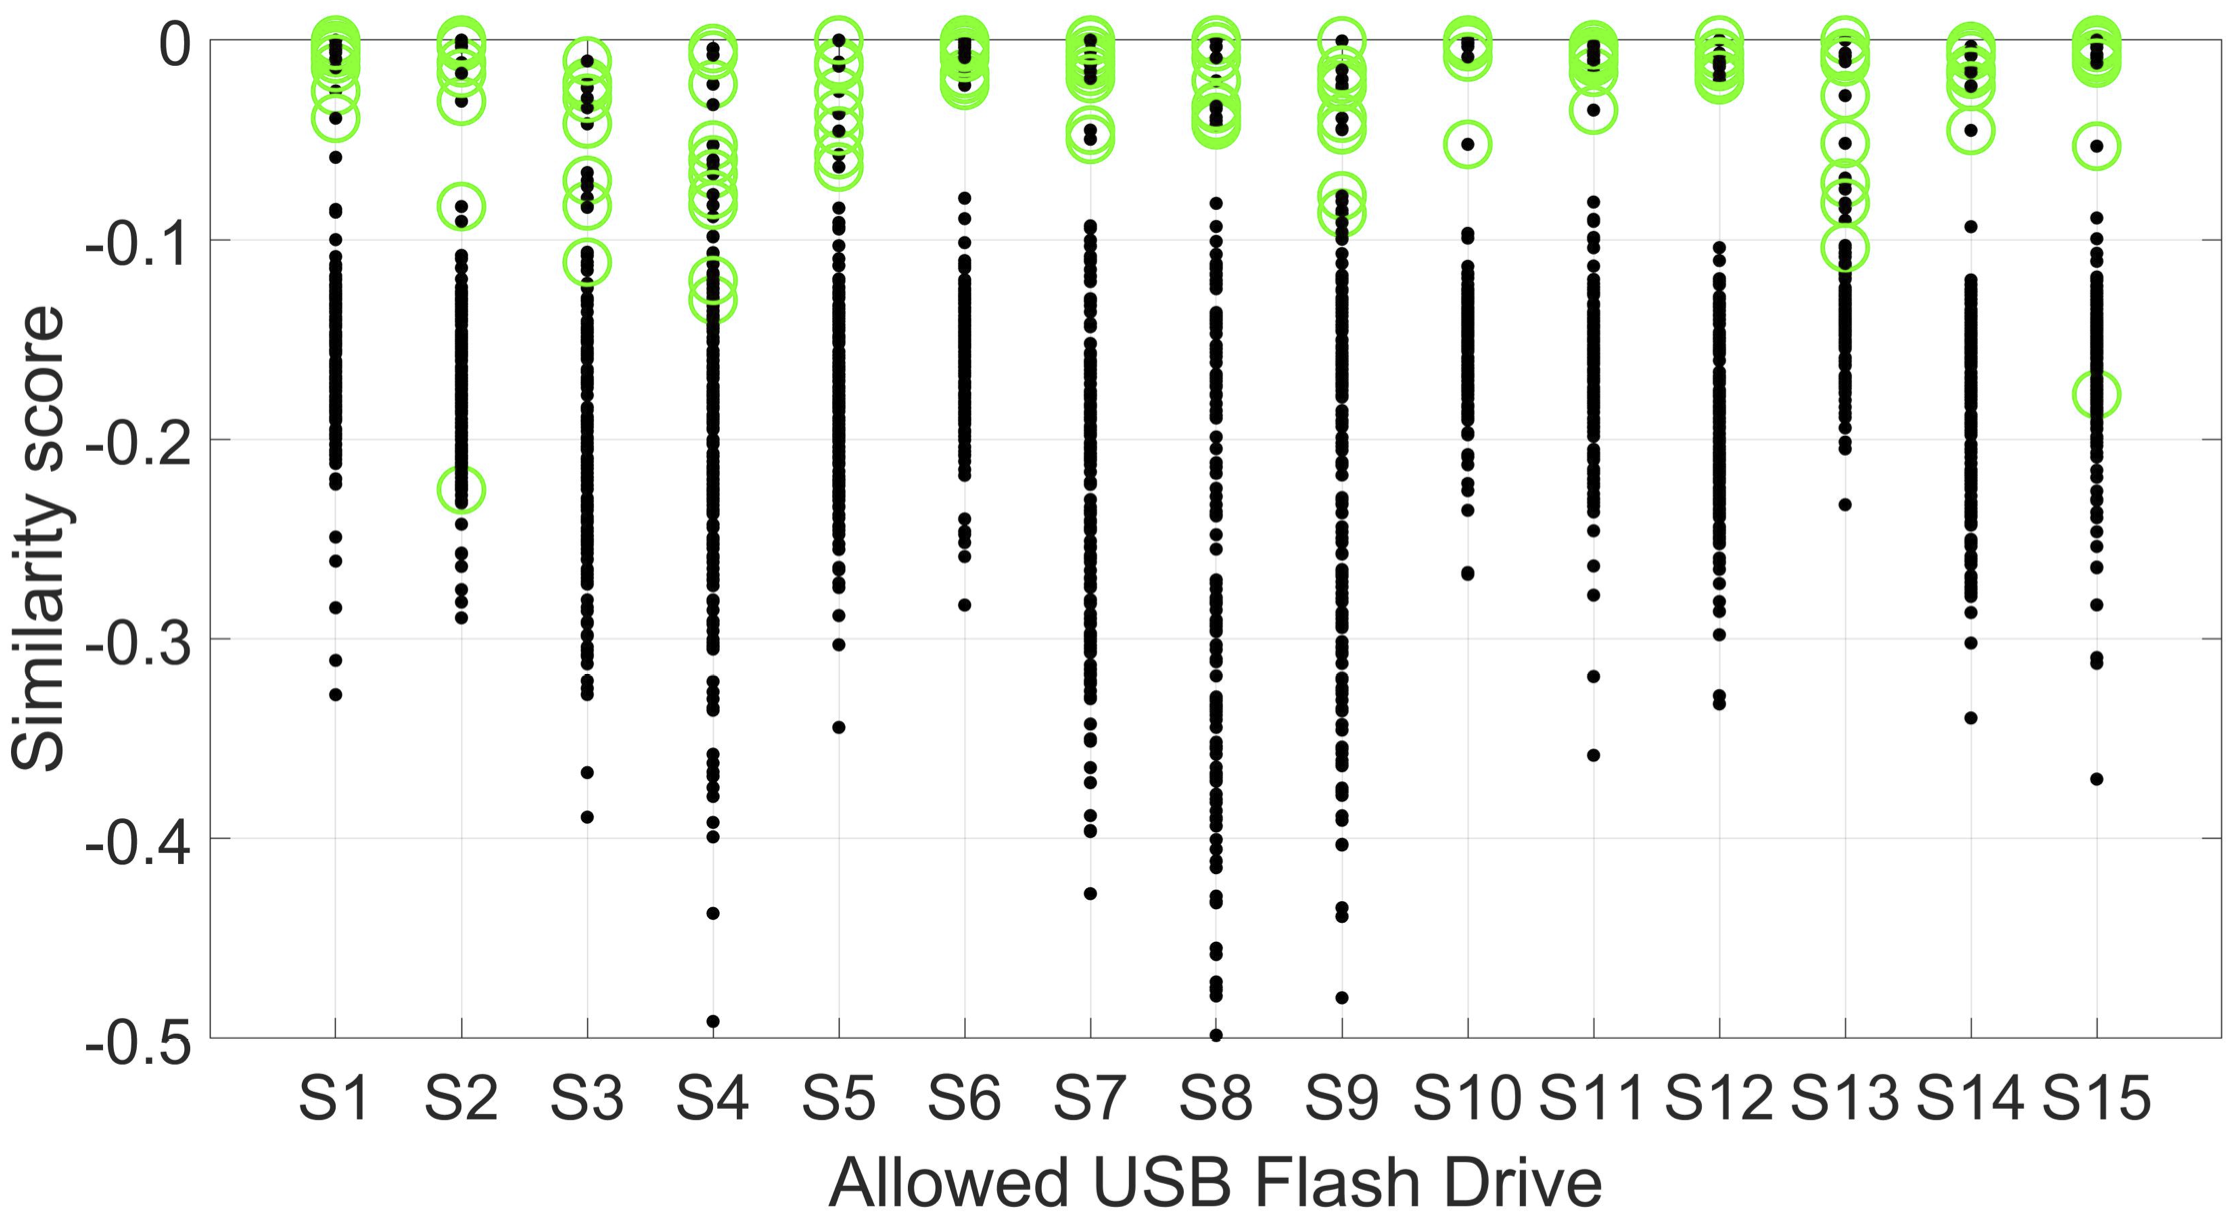
\includegraphics[width=.6\columnwidth]{Figures/scenario2_klevv_final.png}
    \centering
    \caption{Classification accuracy of \sol\ considering 15 Klevv Neo C20 16GB USB Flash Drives.}
    \label{fig:scenario2_klevv}
\end{figure}
% SanDisk    TPR 94.6% FPR 1.9 %
%Strontium   TPR 91.3% FPR 2.7% (opt. TPR 94% FPR 0.5%)
%Klevv        TPR 96%   FPR 1.2%
Figures~\ref{fig:scenario2_sandisk}-\ref{fig:scenario2_klevv} show that most of the (authorized) green circles are characterized by evaluation scores higher than the black (unauthorized) dots. Generally speaking, the selection of the threshold is a key component to determine the accuracy of the devised brands classification method. Low values of the threshold guarantee zero false positives, i.e., no unauthorized brands are erroneously recognized as authorized, but it also implies an increased number of false negatives, i.e., authorized brands erroneously recognized as unauthorized, and thus experiencing a reduced number of True Positives (correctly authorized brands). As a worst-case, we notice that selecting a common threshold $T=-0.09$ for all the SanDisk, the Strontium, and the Klevv Neo, it is possible to guarantee a True Positive Ratio of $0.946$, $0.913$, and $0.963$, and a False Positive Ratio of $0.019$, $0.027$, and $0.012$, respectively. We notice that this is the worst-case, as a threshold can be selected appropriately for each single USB Flash Drive. As an example, with the Strontium USB flash drive, an appropriate choice of the thresholds for each flash drive (that can be done looking at Figure~\ref{fig:scenario2_strontium}) can provide up to TPR $0.94$ and FPR $0.005$. Overall, based on the specific USB flash drive, the network administrator can setup \sol\ in a way to achieve the best trade-off between the TPR and the FPR, to minimize the false positives. In addition, the administrator can also suggest a specific brand to be used for authentication, based on the achievable ratio between the TPR and the FPR.

Finally, we remark that discriminating against the specific USB device requires more powerful equipment than a simple SDR. Specifically, the equipment to be used should be characterized by a wide real-time resolution bandwidth, of about 200 MHz. Despite in our experimental assessment we used the \emph{Rohde \& Schwarz FSW8} spectrum analyzer, other cheaper devices are available, characterized by a similar bandwidth range, with a price starting from as low as 500 USD.

\subsection{Considerations on Features Reduction}
\label{sec:exp_fr}
As previously highlighted, \sol\ requires a total number of 325 features to achieve the reported performances. The reported number of features could appear high, with the risk of incurring in the curse of dimensionality and subsequent model overfitting.

First, we highlight that the methodology adopted by \sol\ is based on the split of the whole data set into multiple disjoint training and test sets. Specifically, for each test, the model of each USB Flash Drive is trained on $9$ samples and tested on the remaining one. This approach is then iterated, by testing each available sample as a test set (while the others serve as a training set). It is worth noting that the model has not been updated after the testing, and we did not refine the hyper-parameters of the one-class SVM classifier (being these two among the common sources of overfitting). Therefore, we can reasonably exclude the hypothesis of overfitting.

However, to provide further insights, we investigated the effectiveness of \sol\ using a reduced number of features, both for Scenario 1 and a reference example for Scenario 2. To determine the critical features, we rank them with the help of the FEAST toolbox, which is a commonly used feature ranking tool in machine learning~\cite{brown2012_jmlr}.  This toolbox has been used also recently by the authors in~\cite{Cheng2019_ccs}, to reduce the dimensionality of the features in the context of unintentional magnetic emissions.
The following Table~\ref{tab:scenario1_fr} and Table~\ref{tab:scenario2_fr} show the results of our investigation with a different number of pre-dominant features, assuming the Scenario 1 (brand and model identification) and the worst-case of Scenario 2 (USB authentication, 15 Strontium USB Flash Drives), respectively. In the tables, we also report the correspondent selection of the threshold value (worst-case), set up to achieve the reported results.

\begin{table}[htbp]
\caption{True Positive Ratio (TPR) and False Positive Ratio (FPR) of \sol\ for the Scenario 1 (brand and model identification), using an increasing number of pre-dominant features, obtained with the FEAST toolbox.
}
\centering
\color{black}
    \begin{tabular}{|c|P{3.0cm}|P{2.2cm}|P{3.1cm}|}
    \hline
        \textbf{No. of Features} & \textbf{Threshold Value} & \textbf{TPR} & \textbf{FPR} \\ \hline
        10     & T = -0.015 & 0.770 & 0.0003 \\
        20     & T = -0.015 & 0.935 & 0.0014 \\
        50     & T = -0.06  & 0.929 & 0.0018 \\
        100    & T = -0.07  & 0.911 & 0.0025 \\
        200    & T = -0.07  & 0.947 & 0.0029 \\
        300    & T = -0.078 & 0.976 & 0.0051 \\
        325    & T = -0.078 & 0.982 & 0.0022 \\
        \hline
    \end{tabular}
    \label{tab:scenario1_fr}
\end{table}
\begin{table}[htbp]
\caption{True Positive Ratio (TPR) and False Positive Ratio (FPR) of \sol\ for the Scenario 2 (USB authentication), in the case of 15 Strontium USB flash drives, using an increasing number of pre-dominant features, obtained with the FEAST toolbox.
}
\centering
\color{black}
    \begin{tabular}{|c|P{3.0cm}|P{2.2cm}|P{3.1cm}|}
    \hline
        \textbf{No. of Features} & \textbf{Threshold Value} & \textbf{TPR} & \textbf{FPR} \\ \hline
        10     & T = -0.8  & 0.753 & 0.040 \\
        20     & T = -0.9  & 0.78  & 0.026 \\
        50     & T = -0.9  & 0.78  & 0.026 \\
        100    & T = -0.9  & 0.893 & 0.041 \\
        200    & T = -0.93 & 0.893 & 0.028 \\
        300    & T = -0.93 & 0.913 & 0.027 \\
        325    & T = -0.93 & 0.913 & 0.027 \\
        \hline
    \end{tabular}
    \label{tab:scenario2_fr}
\end{table}
We notice that the fluctuations of the results by increasing the number of features is limited. For the Scenario 1, the most representative 20 features are enough to obtain a TPR of $0.93$, with a negligible fraction of false positive (FPR $0.0014$). At the same time, for the case of Scenario 2, assuming to work with the Strontium USB Flash Drives, $100$ features are enough to obtain a TPR of $0.893$, and including more features has only a slight impact on the performance accuracy.

Based on the above considerations and results, we believe that we are both avoiding the curse of dimensionality, and not overfitting the model.

\subsection{Discussion on Firmware Modifications}
\label{sec:fw_mod}
As highlighted in Section~\ref{sec:scenario_adv_model}, the firmware of commercial USB flash drives is usually protected by multiple security layers, and cannot be modified. Despite several tutorials are available on media and technical blogs regarding firmware modification of commercial USB flash drives, this is possible only due to vulnerabilities affecting specific versions of the firmware of the USB flash drive. As a direct consequence, the aforementioned vulnerabilities are usually (and immediately) fixed by the vendor.

However, there are specific USB flash drives, such as the Rubber Ducky, whose firmware is specifically designed to be modified to achieve several tasks. These tasks can include benign operations, such as the opening of a file, or malicious activities, such as the disabling of anti-virus software on the host, or the activation of passwords stealing tool.

To provide more insights on the performance of \sol\ to identify modified firmware versions, we investigated the effectiveness of our solution considering seven (7) different firmware versions of the Rubber Ducky (U7):
\begin{itemize}
    \item F1. Baseline default firmware used in Section~\ref{sec:class_usb}, injecting an empty payload; 
    \item F2. Firmware that opens a text file and types a single \emph{Hello World} line;
    \item F3. Firmware that opens a text file and types 100 \emph{Hello World} lines;
    \item F4. Firmware that opens a text file and types 200 \emph{Hello World} lines;
    \item F5. Firmware that disables Windows Defender;
    \item F6. Firmware that inserts a delay of approximately $750$~ms;
    \item F7. Firmware that steals browser-stored passwords.
\end{itemize}
First, we investigated the performance of \sol\ to identify the above firmware modifications, without any previous knowledge of their existence. To this aim, we used the models created for the tests in Section~\ref{sec:class_usb}, while the test set consisted of $10$ acquisitions for the firmware versions \{$F2, \ldots, F7$\}. The results are reported in Figure~\ref{fig:modifiedRD_all}. Note that all the markers are now black dots, as the whole test set samples are considered to be \emph{unauthorized}.
\begin{figure}[htbp]
    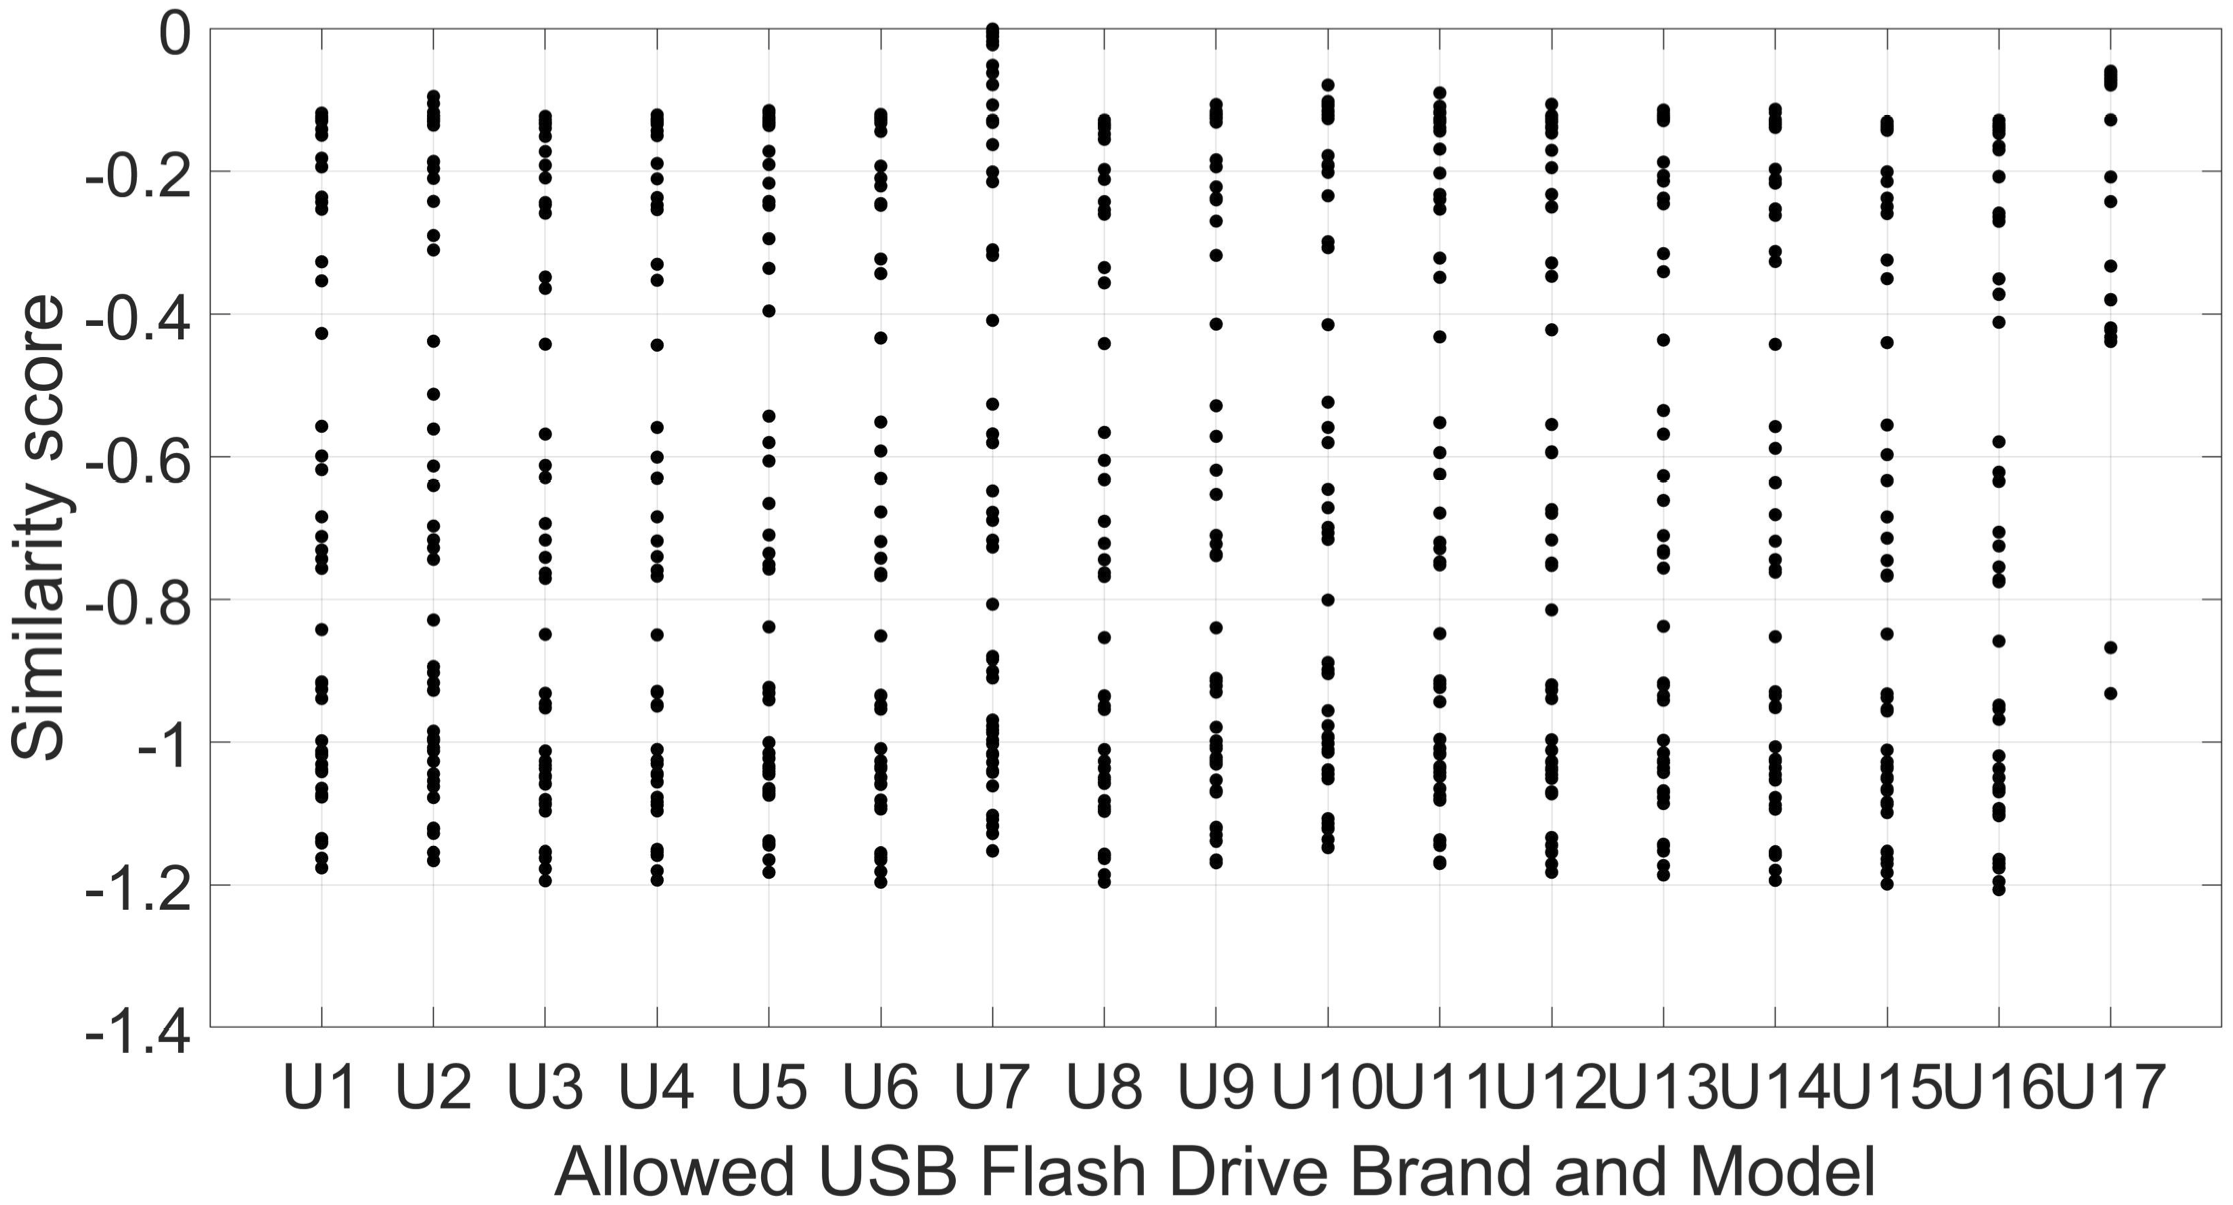
\includegraphics[width=.6\columnwidth]{Figures/modified_RD_all_final.png}
    \centering
    \caption{Classification accuracy of \sol\ considering 6 modified versions of the boot firmware of the Rubber Ducky USB Flash Drive (U7).}
    \label{fig:modifiedRD_all}
\end{figure}
First, we notice that for all the experiments that assume as \emph{authorized} a USB flash drive that is different than the \emph{U7}, report values that are lower than $-0.01$. 
Considering the configuration of the threshold discussed in Section~\ref{sec:class_usb}, these experiments all provide correct \emph{True Negative} outputs. Considering the USB flash drive $U7$, we notice that, out of $50$ experiments, $13$ report values that exceed the local threshold $T=-0.0365$, i.e., the local threshold value obtained from the experiments in Section~\ref{sec:class_usb}, providing FPR $0$. 
These experiments correspond to the firmware $F2$ (8 experiments) and $F5$ (5 experiments). Therefore, in the absence of any training on the modified firmware versions, \sol\ can discriminate a modified firmware only if the profile of the corresponding EM emanations is consistently different from the \emph{trained} one. When the modifications are very little, such as for $F2$ and $F5$, the accuracy of \sol\ decreases.

However, we notice that the accuracy of \sol\ can be significantly enhanced by training on the modified firmware versions. When this is possible (as for the Rubber Ducky), Figure~\ref{fig:modifiedRD_trained} provides the results of such a scenario, using the same procedure used for the previous sections.
\begin{figure}[htbp]
    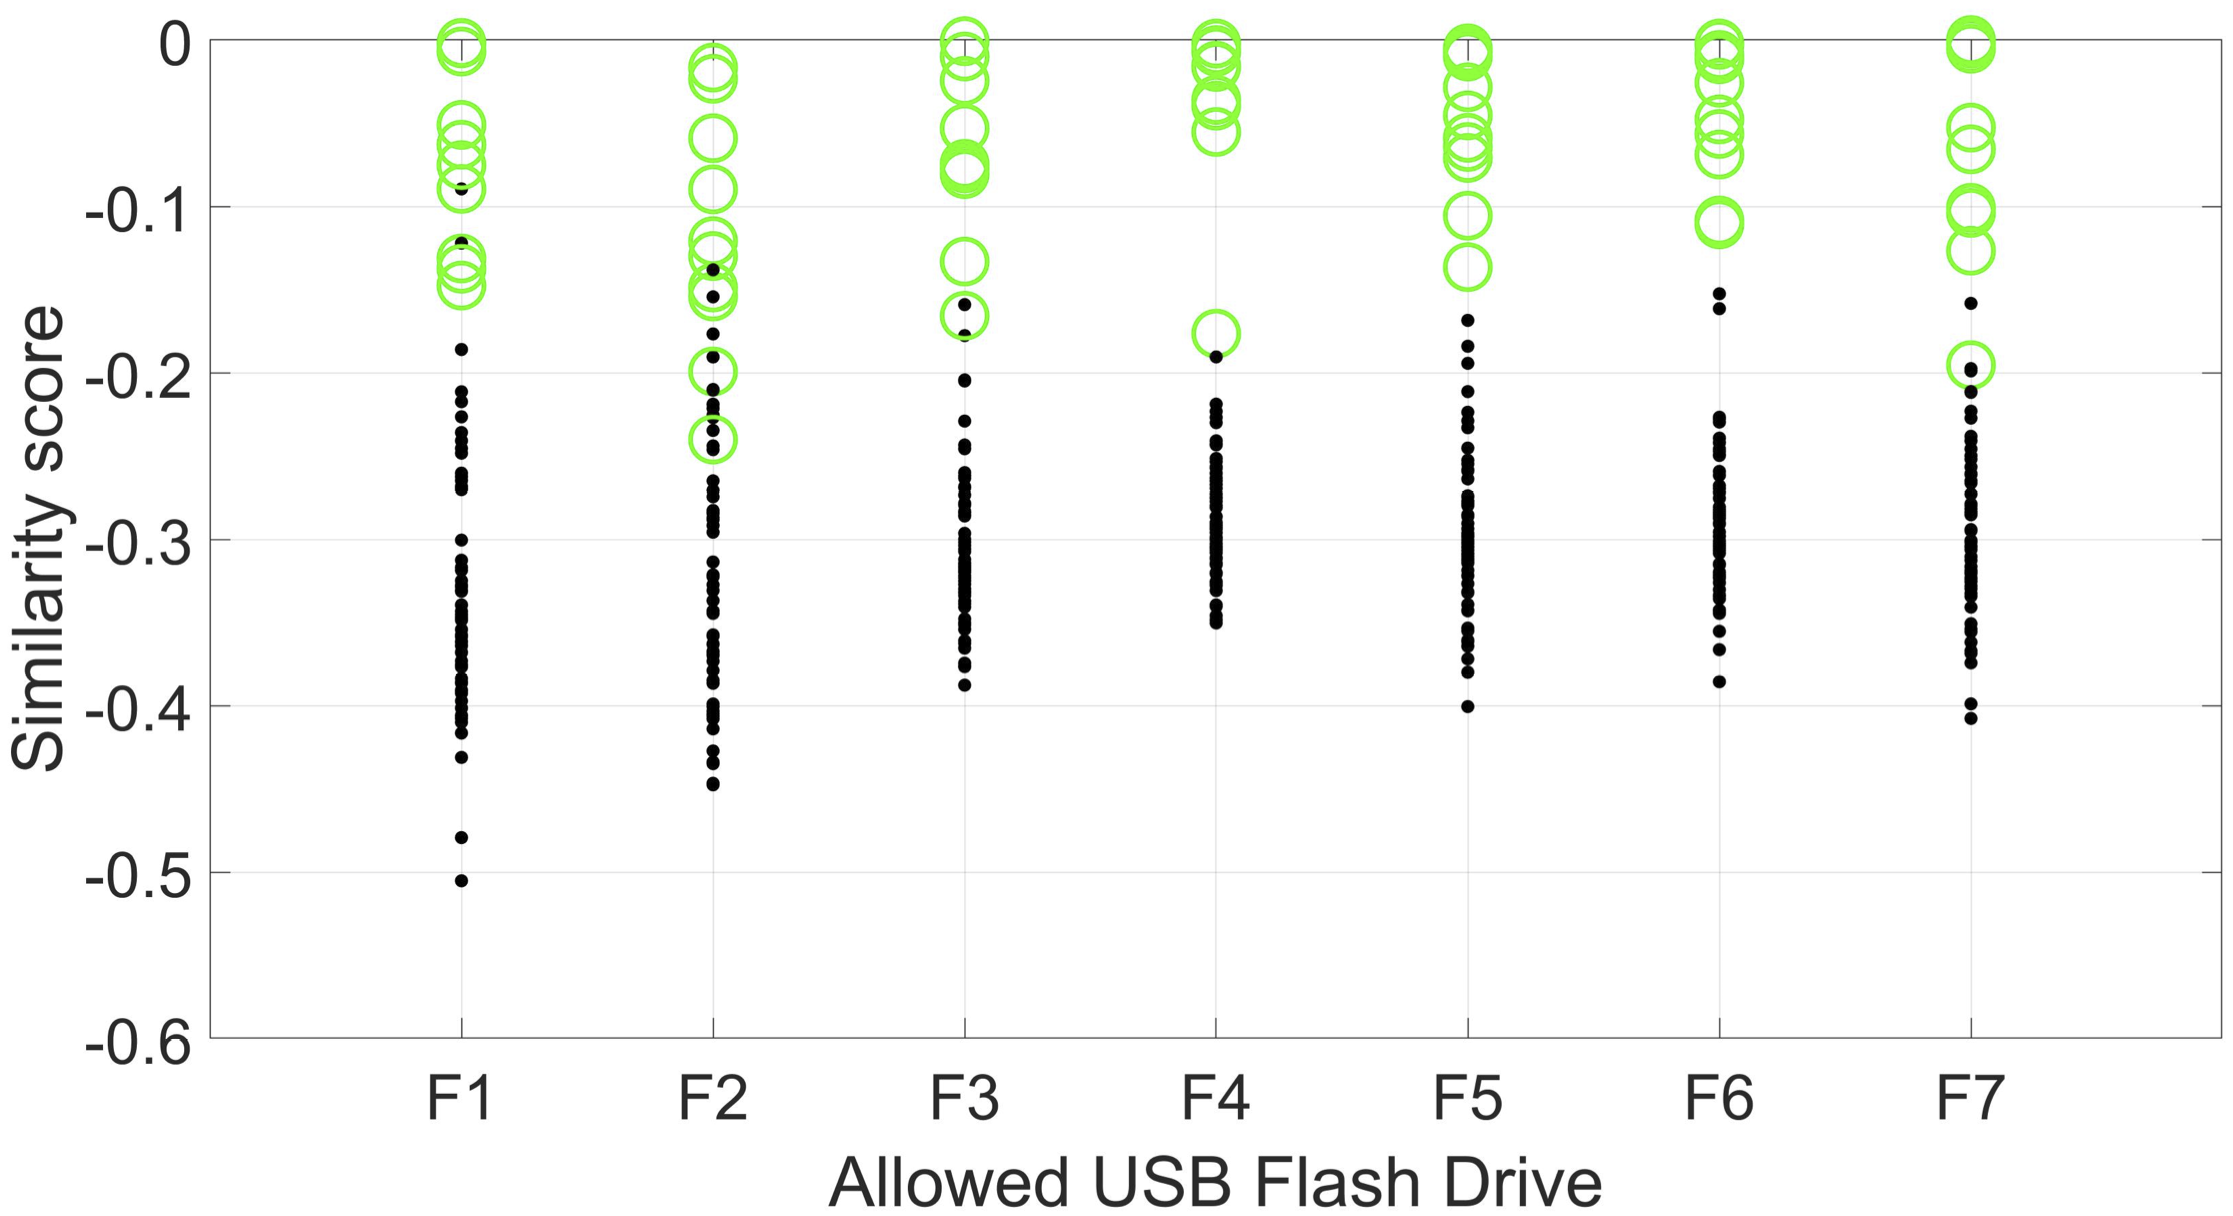
\includegraphics[width=.6\columnwidth]{Figures/modified_RD_trained_final.png}
    \centering
    \caption{Classification accuracy of \sol\ considering 6 modified versions of the boot firmware of the Rubber Ducky USB Flash Drive (U7), assuming to train on the modified firmware versions.}
    \label{fig:modifiedRD_trained}
\end{figure}
It is worth noting that selecting the previously adopted threshold value, i.e. $T=-0.07$, \sol\ achieves FPR $0$, i.e., it does not mislead any of the firmware versions with the native firmware version $F1$ for the USB flash drive $U7$.

\subsection{Host Device (Verifier) configuration and its impact on \sol.}
\label{sec:host_impact}

The analysis and results reported in the previous sections have been obtained using a single host device, as detailed in Section~\ref{subsec:tools}.
This is consistent with the two scenarios and the system model assumed in our work. Indeed, both in a company (Scenario \#1) and in a critical infrastructure (Scenario \#2), it is reasonable to assume that the system administrator has full control of the verifier, i.e., the system used to acquire the fingerprints of the legitimate USB devices and to test new USB devices. Moreover, it is reasonable and convenient for the system administrator that such a system uses the same \acl{OS} of the system(s) used within the site.

To provide further insights about the fingerprinting process, in this subsection, we extend our analysis, investigating the consistency of the fingerprinting process when the hardware and the software of the host devices change.

% different OS
As a reference example, we investigated the consistency of the magnetic emissions radiated during the boot process by a USB flash drive when different versions of the same OS are used on the same machine. To this aim, we collected the unintentional magnetic emissions radiated during the boot of a sample USB flash drive, i.e., the SanDisk Cruzer 128GB drive (U10), when connected to the same machine used for the previous tests, operating with the Windows 7 and the Windows 10 OS. The former includes the version 6.1.7601.1910 of the USB driver, dating back to June 2006, while the latter mounts the latest available version at the time of this writing, i.e., the version 10.0.18362.1 of the USB driver (March 2019). The profiles are shown in Fig.~\ref{fig:diff_os}.
\begin{figure}[htbp]
\centering
    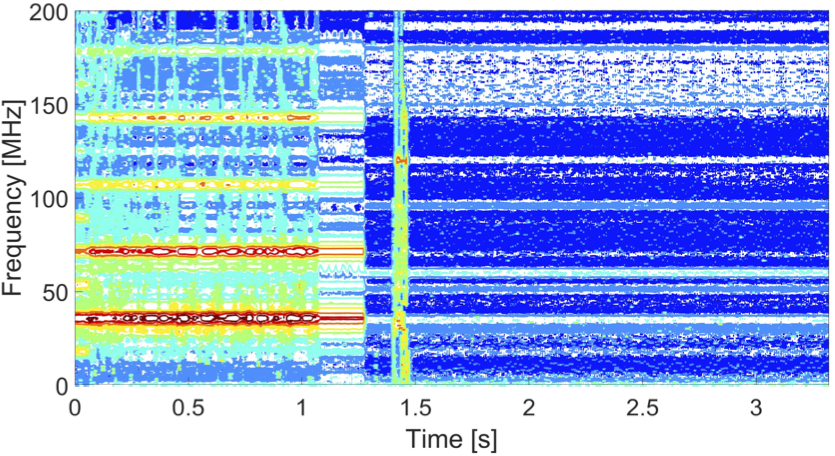
\includegraphics[width=.45\columnwidth]{Figures/SA128W10.png}
    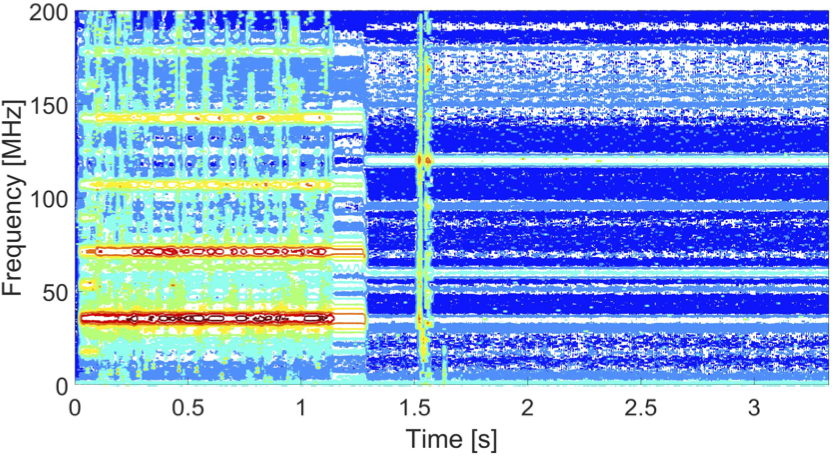
\includegraphics[width=.45\columnwidth]{Figures/SA128W7_002.png}
    \centering
    \caption{Magnetic emissions of a USB flash drive (SanDisk Cruzer 128GB, U10), on (a) Windows 10 OS; and, (b) Windows 7 OS.}
    \label{fig:diff_os}
\end{figure}

Comparing the two figures, some small differences are noticeable, especially in the duration of the different phases of the boot sequence.
We remark that, while we report the figures only for the $U10$ flash drive, the above-described behavior is common to all the USB flash drives analyzed in our work.

Overall, these findings suggest that the construction of the Local Database (i.e., the training process) and the Classification (i.e., the testing process) required by \sol\ should be carried out on the same system, guaranteeing both hardware and software consistency. When at least one of these features changes, differences arise that, especially in the case of Scenario \# 2, could lead to undesired mismatches. Conversely, when the system administrator only requires the verification of the brand and the model of the USB flash drive (Scenario \# 1), fingerprints can be acquired and tested by using different systems or different OSs.

We highlight that these findings are consistent with other related work on unintentional magnetic emissions. Indeed, small modifications to the hardware and software features of involved devices lead to different fingerprints.

% impact of the single components
Overall, our analysis demonstrates that the profile of the unintentional magnetic emissions radiated during the boot procedure is mainly caused by the combination of four main elements: (i) the memory readings/writings of the USB flash drive; (ii) the software instructions executed by the microcontroller chip of the USB flash drive; (iii) the layout of the PCB of the USB flash drive; and, (iv) the hardware and software features of the host device. 
%
This is confirmed by several findings. Considering the same micro-controller chip on a specific host, we have recorded completely different profiles of unintentional magnetic emissions when considering different USB flash drives, characterized by different layout of the PCB. This can be verified by looking at the profile of the unintentional emissions of the devices HP (U1), Kingston (U3), PNY (U5), Patriot (U6), Silicon Power (U13), and Toshiba (U14), sharing the same micro-controller chip but a different layout of the PCB.

%
In addition, as demonstrated by the above analysis, changing the hardware and the software of the host device has a small yet noticeable impact on the fingerprints. When only the software of the host changes, differences in the fingerprint of the same USB flash drive become more pronounced due to a different interaction of the OS with the USB flash drive, affecting the final part of the boot procedure. Considering different hardware (USB flash drive) on the same physical machine, we also experienced small differences in the final part of the boot. 

%
The discussion reported above highlights the effect of the hardware and the software of the host device on the overall recorded fingerprint. However, we remark that the peculiarities associated with the magnetic emissions are both out of the scope of our work and technically hard to achieve when working with System-on-Chip (SoC), such as the USB flash drives.
Indeed, matching the effect of every single electronic component to the fingerprint would require isolating the effect of each of them on the PCB of the specific USB flash drive. This is very hard to achieve both via hardware and software. As for the hardware, disconnecting its components turns out to be very difficult to achieve, in particular when working with SoC, such as the USB flash drives, where all the electronic components are integrated on the same PCB. Disabling the components via software, instead, would require having strict control over the firmware and the software of the USB flash drive. However, they are not accessible by end-users and protected against source code reverse-engineering by multiple security layers.

%
Overall, we can conclude that the differences among the brands and the devices of the same brand are due to small circuits differences, as well as inaccuracies and imperfections in the manufacturing process. On the one hand, the underlying process behind MAGNETO can be brought back to a specific use-case of the Electro-Magnetic emanations of embedded circuits. On the other hand, we would like to recall that our work aims to identify either the brand and the model or the specific USB device, including all the interacting components, as a unique device. Thus, analyzing the effect of each component of the leakage is out of scope for our work. We also remark that \sol\ is novel compared to other related work as, to the best of the authors' knowledge, it is the first solution that can fingerprint USB flash drives in a non-interactive, minimal-invasive, and privacy-preserving fashion, not requiring any intervention or modification on the devices under test.\\
We also highlight that \sol\ can be further extended to interact with the host OS, to instruct the sampling of the unintended magnetic emissions radiated by a connected USB flash drive asynchronously, e.g., when a suspected activity is recorded by the host OS via software. In such a scenario, it could be possible to compare the recorded profile of the specific USB flash drive in regular operating conditions with the actual one, to identify eventual deviations. However, this extension is left as future work.
Finally, we highlight that our methodology, i.e., fingerprinting the device as a whole, without considering the effect of the single components, is consistent with all the related work investigating physical-layer fingerprinting and unintentional Electro-Magnetic emissions, including ~\cite{Dejean2007, camurati2018, cobb2010, Cobb2012_tifs, wright2014, bihl2016, Dubendorfer2012, ramsey2012, Suski2008, lukacs2015, Cheng2019_ccs}. The physical effects underpinning these phenomena are described by the physics fundamental Maxwell equations, and also specific mathematical models are available in the literature, describing their complex creation \cite{bole2009}.

\section{Discussion and Limitations}
\label{sec:discussion}

The results presented in Section \ref{sec:experiments} clearly showed the effectiveness of \sol. We showed that, considering a specific host device, the unintentional magnetic emissions radiated at low frequencies during the boot by a USB flash drive are: (i) very similar for devices of the same brands, (ii) unique for each device, and (iii) consistent in time, thus being a viable and effective tool for USB brand and device fingerprinting. 
For instance, assuming the reference scenario of a company, such as the \emph{Scenario \# 1} discussed in Section \ref{sec:scenario_adv_model}, the system administrator can enforce the use of only specific brands and models of USB flash drive, eventually provided by the company itself. To this aim, the system administrator can deploy \sol\ on a dedicated machine, acquiring the profile of the unintentional magnetic emissions of the selected USB flash drives, before their use.
Then, in the case of a company, on a selected period (e.g., once a day), every time a USB flash drive needs to be used, the system administrator can plug the device into a dedicated laptop, connected to the proposed \sol\ system. Then, if the magnetic emissions at low frequencies during the boot operations match the stored profile for the particular brand and model, the use of the particular USB flash drive could be authorized; otherwise, it will not. 
Similarly, in a critical infrastructure, such as in the \emph{Scenario \# 2} discussed in Section \ref{sec:scenario_adv_model}, it is possible to deploy \sol\ by using powerful equipment, able to acquire the profile of the magnetic emissions on a wider frequency span. As shown in Section \ref{sec:auth}, using such an increased frequency span can enhance the capabilities of \sol, to provide the identification of the specific USB drive.
\\
% \textbf{Qualitative Comparison with Certificate-based Solutions.} A certificate-based authentication solution for USB 2.0 and USB 3.0 devices would require the setup of a dedicated Public Key Infrastructure (PKI), including a trusted Certification Authority (CA) between all the manufacturers of USB devices. According to well-known principles of Public Key Cryptography, this CA would be in charge of signing and releasing public key certificates for each USB device already commercialized. At the same time, the verification of the authenticity of a USB flash drive would require the installation of the public key of the CA in each potential host device, e.g., laptop, workstations, USB-enabled equipment, to name a few, via a dedicated update of the driver of the USB controllers. 
% %
% \\
% %
% This methodology has several drawbacks. From the perspective of the manufacturers of the USB flash drives, the setup of a dedicated PKI to secure the already deployed devices would be highly expensive, and it would cause management issues due to the possible recall of millions of devices. Besides, it would require an agreement between all the manufacturers. From the end-user perspective, this solution would be almost impractical, as it would require the firmware update of each USB flash drive (to be done by the specific user) and the upgrade of the USB controllers of each potential host device (to be done by microchips producers). This is why the deployment of a dedicated PKI is unlikely to happen for USB 2.0 and USB 3.0 devices already commercialized, and, in the best case, it would be practical, still at a high cost, only for future devices, without any update of already commercialized devices. 
% %
% %
% Compared to the aforementioned solution, \sol\ provides several advantages. Indeed, \sol\ emerges as a transparent, easy-to-use, and relatively cheap solution, that is implicitly retro-compatible with any USB specification. Thus, its usage allows the verification of any USB flash drive, without modifications either to the USB flash drive or to the host devices. 
% We also note that \sol\ can be integrated with existing certificate-based authentication solutions (such as the ones already in place to secure the USB Type-C connections), to provide a second independent authentication factor and further enforce the authentication of any USB device.
\noindent
Another feature of \sol\ is its \emph{linear overhead}, independent of the amount of USB flash drives on the market. 
Indeed, the system administrator needs only to 
generate the profile (according to the procedure detailed in the paper) of the USB he/she wants to add to the whitelist of the authorized USB drives. Once the process committed, any USB drive that is screened requires just the collection of the drive's magnetic profile and its comparison against the profiles in the white-list. The operation has a cost that is linear in the size of the white-list.

\noindent
It is worth noting that the setup of \sol\ is only aimed at protecting and ensuring the authenticity of the boot procedures. This choice allows to timely detect a malicious adversary that: (i) replaces the regular USB flash drive with another one having the same external look and form factor, but a different hardware and (possibly malicious) firmware; and, (ii) can replace the firmware of a legacy USB device with a brand new one, by inserting its own code. Such strategies are common to the vast majority of USB attacks known today, as they are based on the complete replacement of the hardware or the firmware of a regular USB device \cite{Nissim2017}.
%
\\
%
{\bf USB firmware tampering.} Despite some USB flash drives are certified according to FIPS 140-2 Level 2 and Level 3 standards, USB flash drives cannot be considered as protected against tampering. As demonstrated in Section~\ref{sec:fw_mod}, the strength of \sol\ lies in the inherent capability to detect the tampering, as long as the modified firmware causes a profile of the unintended magnetic emissions sufficiently different from the recorded one.\\
Indeed, the adversary might replace the firmware of the USB flash drive with a malicious one, where just the minimum amount of lines have been modified to trigger a specific malware. Despite \sol\ can deal with these modifications by training on the modified firmware versions, we highlight that both the executable file and the source code of the firmware on-board of commercial USB flash drives are usually not modifiable and not accessible by the end-users after the deployment. Even in the unlikely case where an adversary can obtain the file of the compiled firmware, it is hard and impractical to reverse-engineer it to obtain the source code. Indeed, being always protected by intellectual property rights, the source code of such firmware is also secret, protected by multiple security layers deployed at manufacturing time, and not available for public download. Thus, it is unfeasible to obtain it and to deploy the aforementioned attack.

\noindent
% Extension to the idle state
Similarly, another adversarial strategy could consist in smartly modifying the firmware of the legacy USB device, inserting just a code line that postpones the injection of the malicious code after the execution of the boot, i.e., when the USB drive goes in the idle state, waiting for instructions by the host. 
Despite the considerations previously done for the legacy firmware modifications are still applicable to this attack, we also observe that \sol\ can be extended to detect the previously mentioned attack. By simply widening the observation window of the \emph{Emissions Extraction Module} and recording the unintentional magnetic emissions when the USB device is in the idle state, \sol\ can detect any anomalous operations initiated by the USB device, raising an immediate alarm. Thus, \sol\ can be extended to guarantee the safe usage of any USB flash drive over an arbitrarily large time after the USB device has been connected to the host system. 

% Extension to malware triggering after the file transfer
\noindent
More powerful adversaries could adopt more sophisticated strategies. For instance, they could tie the execution of the malicious code to a file transfer operation on the particular USB flash drive. When a file is transferred to (or from) the drive, the malicious code is triggered. The effectiveness of \sol\ against this attack could still be achieved by fingerprinting also a file transfer operation, assuming that a file transfer of a given size leads to the same profile of the unintended radiated emission. To neutralize our countermeasure, the adversary could always trigger the execution of the malicious code in a way to be tied to the size of the file to be transferred (e.g., greater than 10 MB). In this case, \sol\ would be effective only if the profile of the unintentional magnetic emissions for the specific file transfer operation has been recorded and profiled before, during the \emph{Training Mode}. It follows that fingerprinting all these operations would affect also the latency and the usability of \sol, increasing the testing time and the overall size of \sol. 
However, if the attack is triggered only when a specific file stored on the USB is opened, \sol\ cannot be effective without any previous fingerprinting process on that specific file.

\section{Conclusion}
\label{sec:conclusion}

In this paper, we proposed \sol, a framework able to enhance the security level in the usage of USB flash drives. Depending on the used equipment, \sol\ can uniquely identify either the brand and the model of commercial USB flash drives, or the specific USB flash drive, by analyzing unintentional magnetic emissions radiated by the target USB devices during the execution of the boot procedure. %s on a dedicated host device. 
Through extensive experimental measurements on 59 different USB drives---belonging to 17 brands, including the top brands purchased on Amazon in mid-2019--- we demonstrated that a USB flash drive can be fingerprinted by only looking at the magnetic emissions unintentionally radiated during the boot procedure on a given host. 
When coupled with a commercial low-cost \acl{SDR} such as the HackRFOne, \sol\ can identify the specific brand and model of the USB flash drive with a minimum classification accuracy of the $98.2$\%, guaranteeing, at the same time, only $0.01$\% of false positives. When coupled with more expensive equipment, characterized by a wide analysis bandwidth of at least 200 MHz, \sol\ can also identify the specific USB flash drive with a minimum classification accuracy of $91.3$\%. All the results above can be obtained in almost real-time, analyzing a time-frame of at most $3.35$ seconds and requiring a negligible processing time (always less than 1 second on a standard laptop).

Thanks to the reported outstanding performance, \sol\ emerges as a viable option to strengthen the security of any sensitive computing equipment exposed to the threats posed by USB drives, such as the one in a telco-backbone or a power plant, and in general contributing to the security of critical infrastructure systems.

\section*{acknowledgments}
The authors would like to thank the anonymous reviewers, that helped to improve the quality of the manuscript.
This publication was made possible by awards NPRP11S-0109-180242 and GSRA6-1-0528-19046, from the QNRF-Qatar National Research Fund, a member of Qatar Foundation. The findings achieved herein are solely the responsibility of the authors.

\bibliographystyle{ACM-Reference-Format}
\bibliography{bibliography}

\end{document}



% \bibliographystyle{plain} %RS: I will change it back to plainnat after cleaning the theory. it's a bit hard to look at in the meantime.
% \bibliography{bib}
\newpage

%\tableofcontents

\appendix

\section{Identification}\label{sec:id}

In seminal work, \cite{rosenbaum1983central,robins1986new} state sufficient conditions under which causal functions, philosophical quantities defined in terms of potential outcomes $\{Y^{(d)}\}$, can be measured from empirical quantities such as outcomes $Y$, treatments $D$, and covariates $(V,X)$. Colloquially, this collection of sufficient conditions is known as selection on observables. We assume selection on observables in the main text, and Pearl's front and back door criteria in Supplement~\ref{sec:graphical}.

\begin{assumption}[Selection on observables]\label{assumption:selection}
Assume
\begin{enumerate}
    \item No interference: if $D=d$ then $Y=Y^{(d)}$.
    \item Conditional exchangeability: $\{Y^{(d)}\}\indep D \mid X$.
    \item Overlap: if $f(x)>0$ then $f(d \mid x)>0$, where $f(x)$ and $f(d \mid x)$ are densities. 
\end{enumerate}
For $\theta_0^{CATE}$, replace $X$ with $(V,X)$.
\end{assumption}

No interference is also called the stable unit treatment value assumption. It rules out network effects, also called spillovers. Conditional exchangeability states that conditional on covariates $X$, treatment assignment is as good as random. Overlap ensures that there is no covariate stratum $X=x$ such that treatment has a restricted support.
%, similar to \cite{imbens2009identification}. %Figure~\ref{dag:te} presents a representative DAG \cite{pearl1993comment}. 
 To handle $\theta_0^{DS}$, we place a standard assumption in transfer learning.
\begin{assumption}[Distribution shift]\label{assumption:covariate}
Assume
\begin{enumerate}
    \item $\tilde{\text{\normalfont pr}}(Y,D,X)=\text{\normalfont pr}(Y \mid D,X)\tilde{\text{\normalfont pr}}(D,X)$;
    \item $\tilde{\text{\normalfont pr}}(D,X)$ is absolutely continuous with respect to $\text{\normalfont pr}(D,X)$.
\end{enumerate}
\end{assumption}
Populations $\text{\normalfont pr}$ and $\tilde{\text{\normalfont pr}}$ differ only in the distribution of treatments and covariates. Moreover, the support of $\text{\normalfont pr}$ contains the support of $\tilde{\text{\normalfont pr}}$.  An immediate consequence is that the regression $\gamma_0(d,x)=E(Y \mid D=d,X=x)$ remains the same across the different populations $\text{\normalfont pr}$ and $\tilde{\text{\normalfont pr}}$. 

\section{Simulations and program evaluation}\label{sec:experiments}

\subsection{Simulations}

\begin{figure}[ht]
\begin{centering}
     \begin{subfigure}[b]{0.48\textwidth}
         \centering
         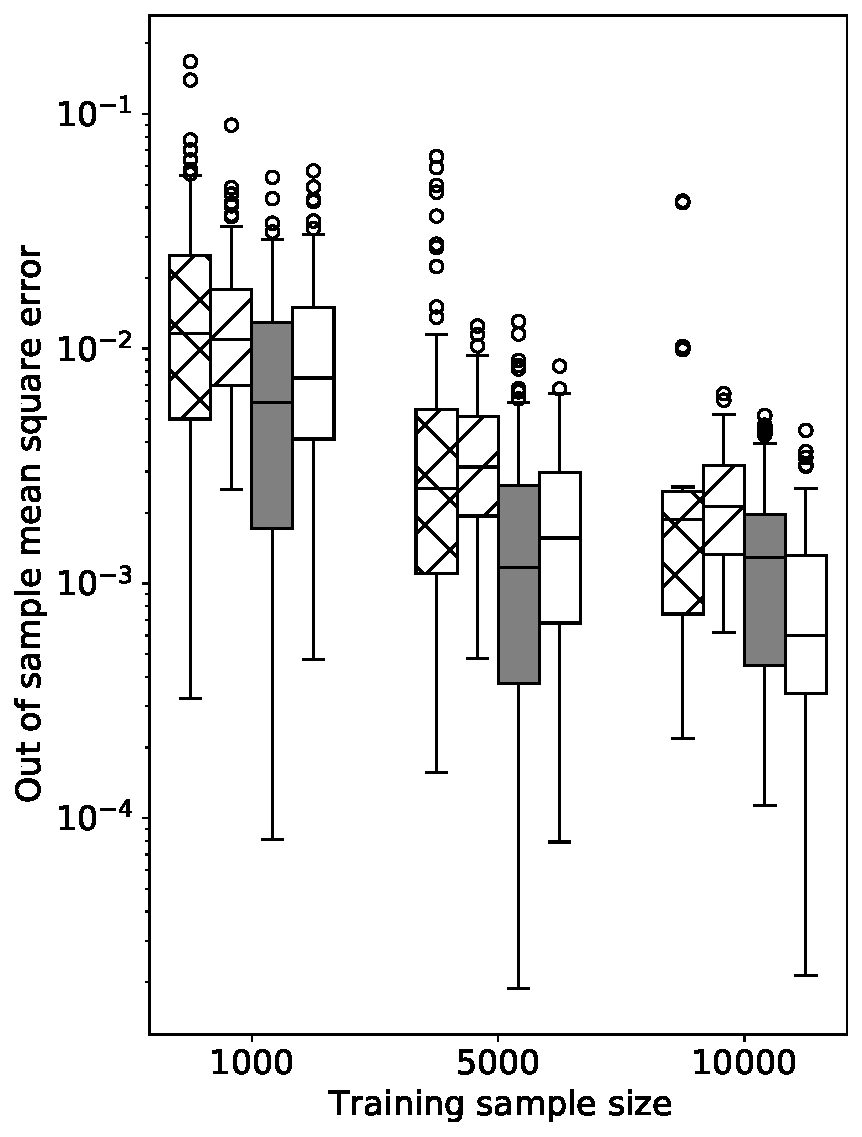
\includegraphics[width=\textwidth]{img/colangelo_all2_sub_rep100_all_bma.pdf}
         %\vspace{-20pt}
         \caption{Dose response curve.}
     \end{subfigure}
     \hfill
     \begin{subfigure}[b]{0.48\textwidth}
         \centering
         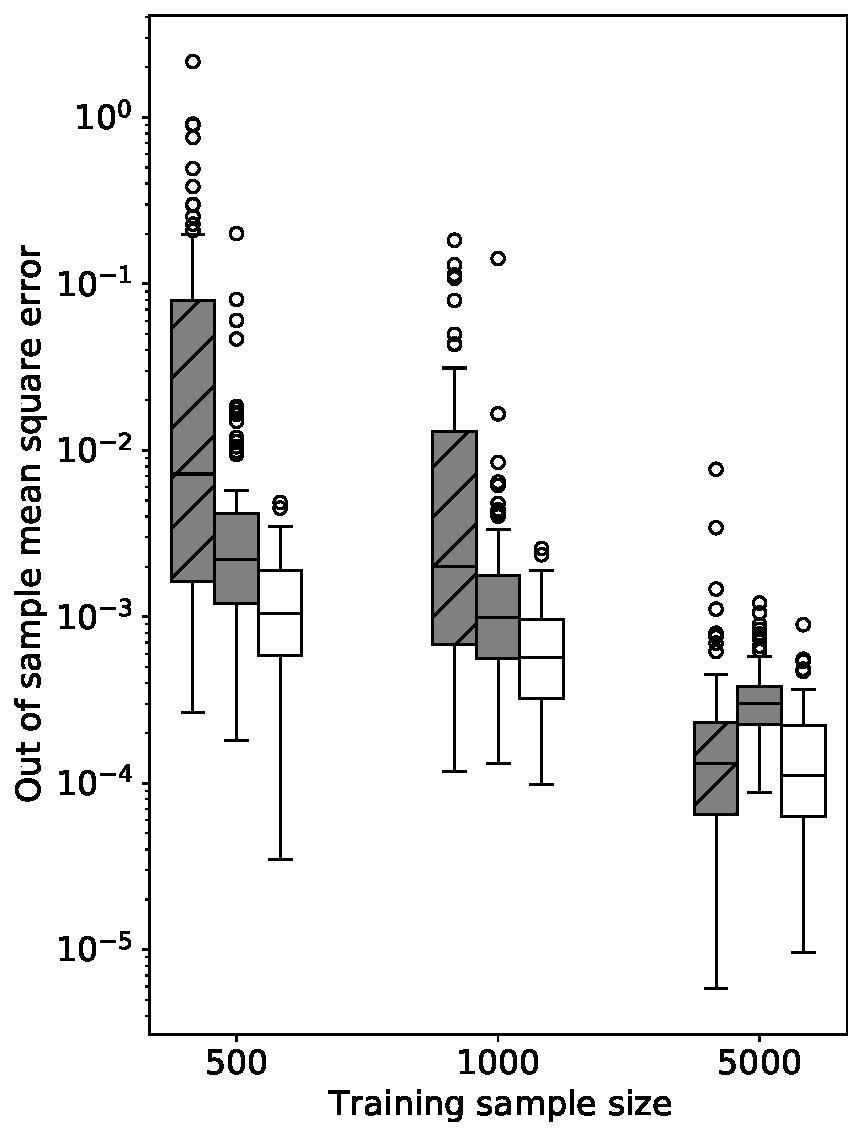
\includegraphics[width=\textwidth]{img/CATE_synthetic2_rep100_all_bma.pdf}
         %\vspace{-20pt}
         \caption{Heterogeneous treatment effect.}
     \end{subfigure}
\par
%\vspace{-10pt}
\caption{\label{fig:cont}
Nonparametric causal function simulations. We implement the estimators of \cite{abrevaya2015estimating} (\texttt{IPW}, lined gray), \cite{kennedy2017nonparametric} (\texttt{DR1}, checkered white), \cite{colangelo2020double} (\texttt{DR2}, lined white), and \cite{semenova2021debiased} (\texttt{DR-series}, gray), in addition to our own (\texttt{RKHS}, white).}
\end{centering}
\end{figure}
We demonstrate that our nonparametric causal function estimators outperform some leading alternatives in nonlinear simulations with many covariates, despite the relative simplicity of our proposed approach. For each causal function design and sample size, we implement 100 simulations and calculate mean square error with respect to the true causal function. Figure~\ref{fig:cont} visualizes results. A lower mean square error is desirable. See Supplement~\ref{sec:simulations} for a full exposition of the data generating processes and implementation details.  

The dose response curve design \cite{colangelo2020double} involves learning the causal function $\theta_0^{ATE}(d)=1.2d+d^2$. A single observation consists of the triple $(Y,D,X)$ for outcome, treatment, and high dimensional covariates where $Y,D\in\mathbb{R}$ and $X\in\mathbb{R}^{100}$. In addition to our one-line nonparametric estimator (\texttt{RKHS}, white), we implement the estimators of \cite{kennedy2017nonparametric} (\texttt{DR1}, checkered white), \cite{colangelo2020double} (\texttt{DR2}, lined white), and \cite{semenova2021debiased} (\texttt{DR-series}, gray). \texttt{DR1} and \texttt{DR2} are local estimators that involve Nadaraya--Watson smoothing around doubly robust estimating equations. \texttt{DR-series} uses series regression with debiased pseudo outcomes, and we give it the advantage of correct specification as a quadratic function. By the Wilcoxon rank sum test, \texttt{RKHS} significantly outperforms alternatives at sample size 10,000, with p value less than $10^{-3}$, despite its relative simplicity.

Though our approach allows for heterogeneous response of a continuous treatment, we implement a design for heterogeneous effect of a binary treatment in order to facilitate comparison with existing methods. The heterogeneous treatment effect design \cite{abrevaya2015estimating} involves learning the causal functions $\theta_0^{CATE}(0,v)=0$ and $\theta_0^{CATE}(1,v)=v(1+2v)^2(v-1)^2$. A single observations consists of the tuple $(Y,D,V,X)$ for outcome, treatment, covariate of interest, and other covariates. In this design, $Y,D,V\in\mathbb{R}$ and  $X\in\mathbb{R}^3$. In addition to our one-line nonparametric estimator (\texttt{RKHS}, white), we implement the estimators of \cite{abrevaya2015estimating} (\texttt{IPW}, lined gray) and \cite{semenova2021debiased} (\texttt{DR-series}, gray). The former involves Nadaraya--Watson smoothing around an inverse propensity estimator, and the latter involves (correctly specified) series regression with a debiased pseudo outcome. The R learner \cite{nie2021quasi} cannot be implemented since $V\neq X$. The simple \texttt{RKHS} approach significantly outperforms alternatives at sample sizes 500 and 1,000 by the Wilcoxon rank sum test, with p values less than $10^{-5}$. 
\subsection{Program evaluation: US Job Corps}


\begin{figure}[ht]
\begin{centering}
     \begin{subfigure}[b]{0.45\textwidth}
         \centering
         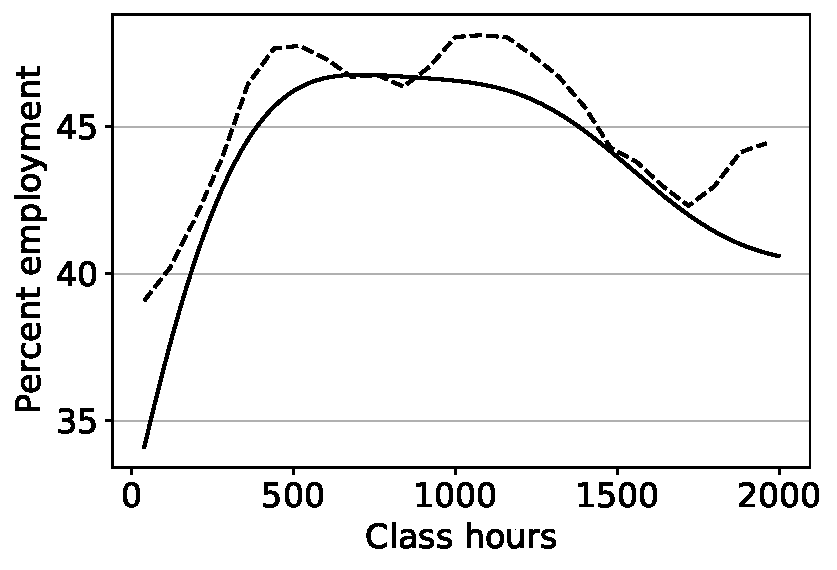
\includegraphics[width=\textwidth]{img/ATE_JCdata_d_filter_with_dml_bma.pdf}
         %\vspace{-20pt}
         \caption{Dose response curve.}
     \end{subfigure}
     \hfill
     \begin{subfigure}[b]{0.45\textwidth}
         \centering
         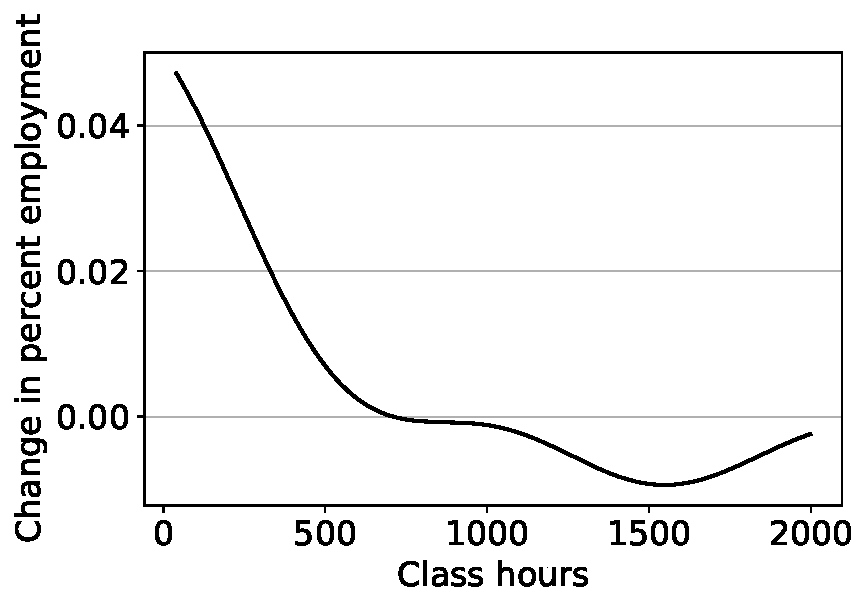
\includegraphics[width=\textwidth]{img/Incremental_ATE_JCdata_d_filter_bma.pdf}
         %\vspace{-20pt}
         \caption{Incremental response curve.}
     \end{subfigure}
     %\vskip\baselineskip
     \begin{subfigure}[b]{0.45\textwidth}
         \centering
         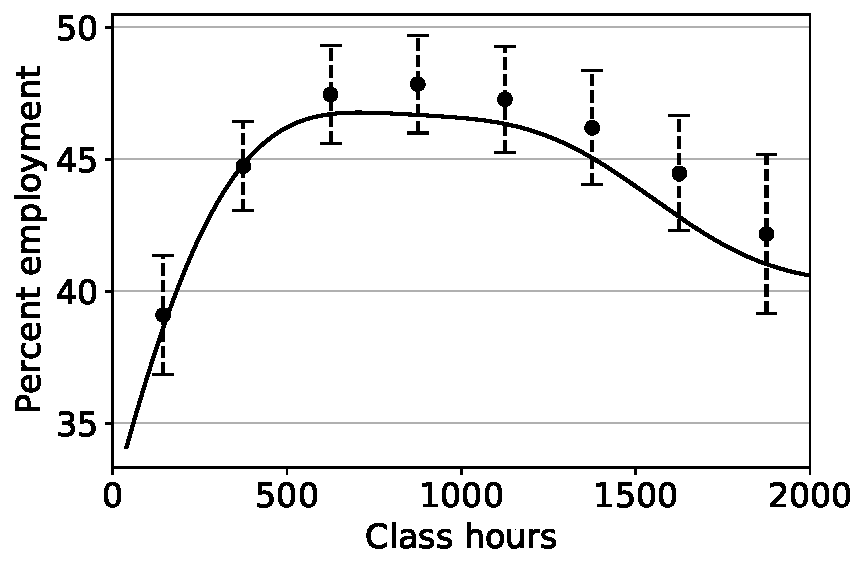
\includegraphics[width=\textwidth]{img/ATE_JCdata_d_filter_ci_fine_gaussian2_bma.pdf}
         %\vspace{-20pt}
         \caption{Discrete treatment effects.}
     \end{subfigure}
     \hfill
     \begin{subfigure}[b]{0.45\textwidth}
         \centering
         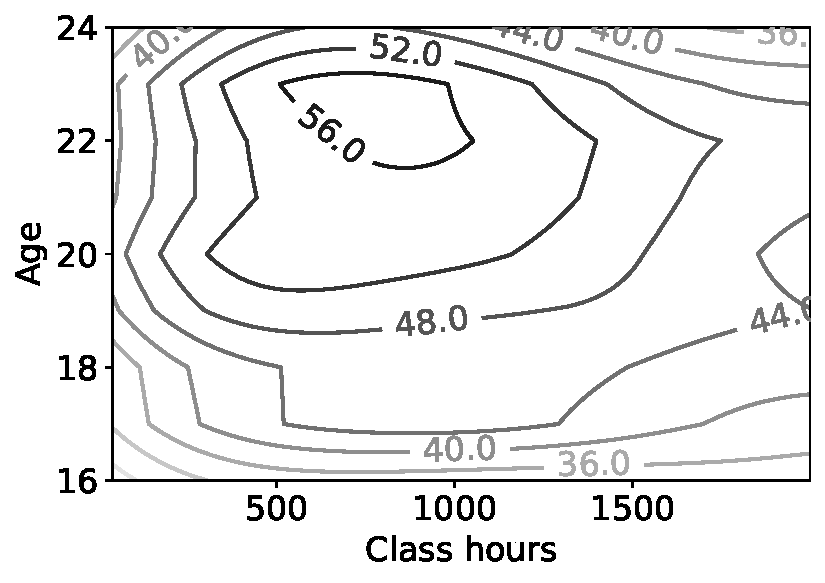
\includegraphics[width=\textwidth]{img/CATE_Age_JCdata_d_filter_bma.pdf}
         %\vspace{-20pt}
         \caption{Heterogeneous response curve.}
     \end{subfigure}
\par
%\vspace{-10pt}
\caption{\label{fig:JC}
Effect of job training on employment. We implement our estimators for dose, heterogeneous, and incremental response curves (\texttt{RKHS}, solid). For comparison, we also implement the dose response curve estimator of \cite{colangelo2020double} (\texttt{DR2}, dashes) as well as the discrete treatment effects of \cite{singh2021debiased} (\texttt{DR3}, vertical bars).}
\end{centering}
\end{figure}

To demonstrate how kernel methods for causal functions are a practical addition to the empirical economic toolkit, we conduct a real world program evaluation. Specifically, we estimate dose, heterogeneous, and incremental response curves of the Jobs Corps, the largest job training program for disadvantaged youth in the US. The Job Corps is financed by the US Department of Labor, and it serves about 50,000 participants annually. Participation is free for individuals who meet low income requirements. Access to the program was randomized from November 1994 to February 1996; see \cite{schochet2008does} for details. Many studies focus on data from this period to evaluate the effect of job training on employment \cite{flores2012estimating,colangelo2020double}. Though access to the program was randomized, individuals could decide whether to participate and for how many hours. From a causal perspective, we assume selection on observables: conditional on observed covariates, participation was exogenous on the extensive and intensive margins. From a statistical perspective, we assume that different intensities of job training have smooth effects on counterfactual employment, and that those effects are smoothly modified by age, assumptions motivated by labor market theory.

In this setting, the continuous treatment $D\in\mathbb{R}$ is total hours spent in academic or vocational classes in the first year after randomization, and the continuous outcome $Y\in\mathbb{R}$ is the proportion of weeks employed in the second year after randomization. The covariates $X\in\mathbb{R}^{40}$ include age, gender, ethnicity, language competency, education, marital
status, household size, household income, previous receipt of social aid, family background, health, and health related behavior at base line. As in \cite{colangelo2020double}, we focus on the $n=3,906$ observations for which $D\geq 40$, i.e. individuals who completed at least one week of training. We implement various causal parameters in Figure~\ref{fig:JC}: the dose response curve; the incremental response curve; the discrete treatment effects with confidence intervals of \cite{singh2021debiased}; and the heterogeneous response curve with respect to age. For the discrete effects, we discretize treatment into roughly equiprobable bins: $[40,250]$, $(250,500]$, $(500,750]$ $(750,1000]$, $(1000,1250]$, $(1250,1500]$, $(1500,1750]$, and $(1750,2000]$ class hours. As far as we know, the heterogeneous response of class hours, a continuous treatment, has not been previously studied in this empirical setting. In Supplement~\ref{sec:application}, we provide implementation details and verify that our results are robust to the choice of sample.

The dose response curve plateaus and achieves its maximum around $d=500$, corresponding to 12.5 weeks of classes. Our global estimate (\texttt{RKHS}, solid) has the same overall shape but is smoother and slightly lower than the collection of local estimates from \cite{colangelo2020double} (\texttt{DR2}, dashes). The smoothness of our estimator is a consequence of the RKHS assumptions, and we see how it is a virtue for empirical economic research; a smooth dose response curve is more economically plausible in this setting. The first 12.5 weeks of classes confer most of the gain in employment: from 35\% employment to more than 47\% employment for the average participant. The incremental response curve (\texttt{RKHS}, solid) is the derivative of the dose response curve, and it visualizes where the greatest gain happens. The discrete treatment effects of \cite{singh2021debiased} (\texttt{DR3}, vertical bars) corroborate our dose response curve, and the 95\% confidence intervals contain the dose response curve of \cite{colangelo2020double} (\texttt{DR2}, dashes) as well as our own (\texttt{RKHS}, solid). 
%By measuring continuous treatment effects rather than binary treatment effects, we are able to determine how many class hours are optimal. 
Finally, the heterogeneous response curve (\texttt{RKHS}, solid) shows that age plays a substantial role in the effectiveness of the intervention. For the youngest participants, the intervention has a small effect: employment only increases from 28\% to at most 36\%. For older participants, the intervention has a large effect: employment increases from 40\% to 56\%. %Again, the first 12 weeks of classes confer the greatest gain. By measuring heterogeneous treatment effects, we are able to determine the subpopulation for whom class hours are most effective. 
Our policy recommendation is therefore 12--14 weeks of classes targeting individuals 21--23 years old.

\section{Counterfactual distributions}\label{sec:distribution}

\subsection{Definition}

In the main text, we study causal functions defined as means of potential outcomes. In this section, we extend the estimators and analyses presented in the main text to counterfactual distributions of potential outcomes. A counterfactual distribution can be encoded by a kernel mean embedding using a new feature map $\phi(y)$ for a new scalar valued RKHS $\mathcal{H}_{\mathcal{Y}}$. We now allow $\mathcal{Y}$ to be a Polish space (Assumption~\ref{assumption:original}).
\begin{definition}[Counterfactual distributions and embeddings] We define %the distribution effects and their mean embeddings by
\begin{enumerate}
    \item Counterfactual distribution: $
\theta_0^{D:ATE}(d)=\text{\normalfont pr}\{Y^{(d)}\}
$ is the counterfactual distribution of outcomes given intervention $D=d$ for the entire population.
    \item Counterfactual distribution with distribution shift: $
\theta_0^{D:DS}(d,\tilde{\text{\normalfont pr}})=\tilde{\text{\normalfont pr}}\{Y^{(d)}\}
$ is the counterfactual distribution of outcomes given intervention $D=d$ for an alternative population with data distribution $\tilde{\text{\normalfont pr}}$ (elaborated in Assumption~\ref{assumption:covariate}).
    \item Conditional counterfactual distribution: $
\theta_0^{D:ATT}(d,d')=\text{\normalfont pr}\{Y^{(d')} \mid D=d\}
$ is the counterfactual distribution of outcomes given intervention $D=d'$ for the subpopulation who actually received treatment $D=d$.
    \item Heterogeneous counterfactual distribution: $
\theta_0^{D:CATE}(d,v)=\text{\normalfont pr}\{Y^{(d)} \mid V=v\}
$ is the counterfactual distribution of outcomes given intervention $D=d$ for the subpopulation with covariate value $V=v$.
\end{enumerate}
Likewise we define counterfactual distribution embeddings, e.g. $
\check{\theta}_0^{D:ATE}(d)=E\{\phi(Y^{(d)})\}.
$
\end{definition}

Our strategy is to estimate the embedding of a  counterfactual distribution. At that point, the analyst may use the embedding to (i) estimate moments of the counterfactual distribution \cite{kanagawa2014recovering} or (ii) sample from the counterfactual distribution \cite{welling2009herding}. Since we already analyze means in the main text, we focus on (ii) in this supplement.

\subsection{Identification}

The same identification results apply to counterfactual distributions.

\begin{lemma}[Identification of counterfactual distributions]\label{theorem:id_treatment_dist}
If Assumption~\ref{assumption:selection} holds,
\begin{enumerate}
     \item $\{\theta_0^{D:ATE}(d)\}(y)=\int \text{\normalfont pr}(y \mid d,x)\mathrm{d}\text{\normalfont pr}(x)$.
    \item If in addition Assumption~\ref{assumption:covariate} holds, then $\{\theta_0^{D:DS}(d,\tilde{\text{\normalfont pr}})\}(y)=\int \text{\normalfont pr}(y \mid d,x)\mathrm{d}\tilde{\text{\normalfont pr}}(x)$.
    \item $\{\theta_0^{D:ATT}(d,d')\}(y)=\int \text{\normalfont pr}(y \mid d',x)\mathrm{d}\text{\normalfont pr}(x \mid d)$ \cite{chernozhukov2013inference}.
    \item $\{\theta_0^{D:CATE}(d,v)\}(y)=\int \text{\normalfont pr}(y \mid d,v,x)\mathrm{d}\text{\normalfont pr}(x \mid v)$.
\end{enumerate}
Likewise for embeddings of counterfactual distributions. For example, if in addition Assumption~\ref{assumption:RKHS} holds, then $\check{\theta}_0^{D:ATE}(d)=\int E\{\phi(Y) \mid D=d,X=x\}\mathrm{d}\text{\normalfont pr}(x)
$.
\end{lemma}
The identification results for embeddings of counterfactual distributions resemble those presented in the main text. Define the generalized regressions
$
\gamma_0(d,x)=E\{\phi(Y) \mid D=d,X=x\}
$ and $\gamma_0(d,v,x)=E\{\phi(Y) \mid D=d,V=v,X=x\}$. Then we can express these results in the familiar form, e.g. $\check{\theta}_0^{D:ATE}(d)=\int \gamma_0(d,x)\mathrm{d}\text{\normalfont pr}(x)$.

\subsection{Closed form solution}

To estimate counterfactual distributions, we extend the RKHS construction in Section~\ref{sec:algorithm}. As before, define scalar valued RKHSs for treatment $D$ and covariates $X$. Define an additional scalar valued RKHS for outcome $Y$. Because the regression $\gamma_0$ is now a conditional mean embedding, we present a construction involving a conditional expectation operator. Define the conditional expectation operator
$
E_3:\mathcal{H}_{\mathcal{Y}}\rightarrow \mathcal{H}_{\mathcal{D}}\otimes \mathcal{H}_{\mathcal{X}},\; f(\cdot)\mapsto E\{f(Y) \mid D=\cdot,X=\cdot \}
$. By construction
$
\gamma_0(d,x)=E_3^*\{\phi(d)\otimes \phi(x)\}
$.  As before, we replace $X$ with $(V,X)$ for $\theta_0^{D:CATE}$. We place regularity conditions on this RKHS construction, similar to those in Section~\ref{sec:algorithm}, to represent counterfactual distributions as evaluations of $E_3^*$. This representation allows for continuous treatment, unlike the representation in \cite[eq. 16, 17, 20]{muandet2021counterfactual}.

\begin{theorem}[Decoupling via kernel mean embeddings]\label{theorem:representation_dist}
Suppose the conditions of Lemma~\ref{theorem:id_treatment_dist} hold. Further suppose Assumption~\ref{assumption:RKHS} holds and $E_3\in\mathcal{L}_2(\mathcal{H}_{\mathcal{Y}},\mathcal{H}_{\mathcal{D}}\otimes \mathcal{H}_{\mathcal{X}})$. Then
\begin{enumerate}
    \item $\check{\theta}_0^{D:ATE}(d)=E_3^*\{\phi(d)\otimes \mu_x\} $ where $\mu_x=\int\phi(x) \mathrm{d}\text{\normalfont pr}(x) $.
    \item $\check{\theta}_0^{D:DS}(d,\tilde{\text{\normalfont pr}})=E_3^*\{\phi(d)\otimes \nu_x\}$ where $\nu_x=\int\phi(x) \mathrm{d}\tilde{\text{\normalfont pr}}(x) $.
    \item $\check{\theta}_0^{D:ATT}(d,d')=E_3^*\{\phi(d')\otimes \mu_x(d)\} $  where $\mu_x(d)=\int\phi(x) \mathrm{d}\text{\normalfont pr}(x \mid d)$.
    \item $\check{\theta}_0^{D:CATE}(d,v)=E_3^*\{\phi(d)\otimes \phi(v)\otimes \mu_{x}(v)\}$ where $\mu_{x}(v)= \int \phi(x) \mathrm{d}\text{\normalfont pr}(x \mid v)$.
\end{enumerate}
For $\theta_0^{D:CATE}$, we instead assume $E_3\in\mathcal{L}_2(\mathcal{H}_{\mathcal{Y}},\mathcal{H}_{\mathcal{D}}\otimes\mathcal{H}_{\mathcal{V}} \otimes  \mathcal{H}_{\mathcal{X}})$.
\end{theorem}


See Supplement~\ref{sec:derivation} for the proof. The mean embeddings are the same as in Theorem~\ref{theorem:representation_treatment}. They encode the reweighting distributions as elements in the RKHS such that the counterfactual distribution embeddings can be expressed as evaluations of $E_3^*$. 

As in Section~\ref{sec:algorithm}, the abstract representation helps to define estimators with closed form solutions that can be easily computed. In particular, the representation separates the three steps necessary to estimate a counterfactual distribution: estimating a conditional distribution, which may involve many covariates; estimating the distribution for reweighting; and using one distribution to integrate another. For example, for $\check{\theta}_0^{D:CATE}(d,v)$, our estimator is $\hat{\theta}^{D:CATE}(d,v)=\hat{E}_3^*\{\phi(d)\otimes \phi(v) \otimes \hat{\mu}_x(v)\}$. $\hat{E}_3$ and $\hat{\mu}_x(v)$ are generalized kernel ridge regressions, and the latter can be used to integrate the former by simply multiplying the two. This algorithmic insight is a key innovation of the present work, and the reason why our estimators have simple closed form solutions despite complicated causal integration.

\begin{algorithm}[Estimation of counterfactual distribution embeddings]\label{algorithm:dist}
Denote the empirical kernel matrices
$
K_{DD}, K_{XX}, K_{YY}\in\mathbb{R}^{n\times n}
$. Let $(\tilde{X}_i)$ $(i=1,...,\tilde{n})$ be observations drawn from population $\tilde{\text{\normalfont pr}}$. Denote by $\odot$ the elementwise product. The distribution embedding estimators have the closed form solutions
\begin{enumerate}
    \item $\{\hat{\theta}_0^{D:ATE}(d)\}(y)=n^{-1}\sum_{i=1}^n K_{yY}(K_{DD}\odot K_{XX}+n\lambda_3  I )^{-1}(K_{Dd}\odot K_{Xx_i})$;
    \item $\{\hat{\theta}_0^{D:DS}(d)\}(y)=\tilde{n}^{-1}\sum_{i=1}^{\tilde{n}} K_{yY}(K_{DD}\odot K_{XX}+n\lambda_3  I )^{-1}(K_{Dd}\odot K_{X\tilde{x}_i})$;
    \item $\{\hat{\theta}_0^{D:ATT}(d,d')\}(y)=K_{yY}(K_{DD}\odot K_{XX}+n\lambda_3  I )^{-1}[K_{Dd'}\odot \{K_{XX}(K_{DD}+n\lambda_1  I )^{-1}K_{Dd}\}]$;
     \item $\{\hat{\theta}_0^{D:CATE}(d,v)\}(y)=K_{yY}(K_{DD}\odot K_{VV}\odot K_{XX}+n\lambda_3  I )^{-1}[K_{Dd}\odot K_{Vv} \odot \{K_{XX}(K_{VV}+n\lambda_2  I )^{-1}K_{Vv}\}]$;
\end{enumerate}
where $(\lambda_1,\lambda_2,\lambda_3)$ are ridge regression penalty hyperparameters.%\footnote{Note that $[\hat{\theta}_0^{D:ATE}(d)](\cdot):\mathcal{Y}\rightarrow \mathbb{R}$ is a function, so $K_{(\cdot) Y}:\mathcal{Y}\rightarrow\mathbb{R}^n$ is a function.} 
\end{algorithm}
We derive these estimators in Supplement~\ref{sec:derivation}. We give theoretical values for $(\lambda_1,\lambda_2,\lambda_3)$ that optimally balance bias and variance in Theorem~\ref{theorem:consistency_treatment} below. Supplement~\ref{sec:tuning} gives practical tuning procedures, one of which is asymptotically optimal. 
%Note that $\hat{\theta}^{D:DS}$ requires observations of covariates from the alternative population $\tilde{\text{\normalfont pr}}$. 
We avoid the estimation and inversion of propensity scores in \cite[eq. 21]{muandet2021counterfactual}.

Algorithm~\ref{algorithm:dist} estimates counterfactual distribution embeddings. The ultimate parameters of interest are counterfactual distributions. We present a deterministic procedure that uses the distribution embedding to provide samples $(\tilde{Y}_j)$ from the distribution. In Theorem~\ref{theorem:conv_dist} below, we prove that these samples converge in distribution to the counterfactual distribution. The procedure is a variant of kernel herding  \cite{welling2009herding,muandet2021counterfactual}.

\begin{algorithm}[Estimation of counterfactual distributions]\label{algorithm:herding}
Recall that $\hat{\theta}_0^{D:ATE}(d)$ is a mapping from $\mathcal{Y}$ to $\mathbb{R}$. 
Given $\hat{\theta}_0^{D:ATE}(d)$, calculate
\begin{enumerate}
    \item $\tilde{Y}_1=\argmax_{y\in\mathcal{Y}} \left[ \{\hat{\theta}_0^{D:ATE}(d)\}(y)\right]$;
    \item $\tilde{Y}_{j}=\argmax_{y\in\mathcal{Y}} \left[ \{\hat{\theta}_0^{D:ATE}(d)\}(y)-(j+1)^{-1}\sum_{\ell=1}^{j-1}k_{\mathcal{Y}}(\tilde{Y}_{\ell},y)\right]$ for $j>1$.
\end{enumerate}
Likewise for the other counterfactual distributions, replacing $\hat{\theta}_0^{D:ATE}(d)$ with the other quantities in Algorithm~\ref{algorithm:dist}.
\end{algorithm}
By this procedure, samples from counterfactual distributions are straightforward to compute. With such samples, one may visualize a histogram as an estimator of the counterfactual density of potential outcomes. Alternatively, one may test statistical hypotheses.

\subsection{Convergence in distribution}

Towards a guarantee of uniform consistency, we place regularity conditions on the original spaces as in Assumption~\ref{assumption:original}. Importantly, we relax the condition that $\mathcal{Y}\subset \mathbb{R}$; instead, we assume $\mathcal{Y}$ is a Polish space. Next, we assume the regression $\gamma_0$ is smooth and quantify the spectral decay of its RKHS, parameterized in terms of the conditional expectation operator $E_3$. Likewise we assume the conditional mean embeddings $\mu_x(d)$ and $\mu_x(v)$ are smooth and quantify their spectral decay. With these assumptions, we arrive at our next main result.
\begin{theorem}[Uniform consistency of counterfactual distribution embeddings]\label{theorem:consistency_dist}
Suppose Assumptions~\ref{assumption:selection},~\ref{assumption:RKHS},~\ref{assumption:original}, and~\ref{assumption:smooth_op} hold with $\mathcal{A}_3=\mathcal{Y}$ and $\mathcal{B}_3=\mathcal{D}\times \mathcal{X}$ (or $\mathcal{B}_3=\mathcal{D}\times \mathcal{V}\times \mathcal{X}$ for $\theta_0^{D:CATE}$). Set $(\lambda_1,\lambda_2,\lambda_3)=\{n^{-1/(c_1+1/b_1)},n^{-1/(c_2+1/b_2)},n^{-1/(c_3+1/b_3)}\}$, which is rate optimal regularization.
\begin{enumerate}
    \item Then with high probability
    $$
    \sup_{d\in\mathcal{D}}\|\hat{\theta}^{D:ATE}(d)-\check{\theta}_0^{D:ATE}(d)\|_{\mathcal{H}_{\mathcal{Y}}}=O\left[n^{-(c_3-1)/\{2(c_3+1/b_3)\}}\right].
$$
 \item If in addition Assumption~\ref{assumption:covariate} holds, then with high probability
      $$
     \sup_{d\in\mathcal{D}}\|\hat{\theta}^{D:DS}(d,\tilde{\text{\normalfont pr}})-\check{\theta}_0^{D:DS}(d,\tilde{\text{\normalfont pr}})\|_{\mathcal{H}_{\mathcal{Y}}}=O\left[ n^{-(c_3-1)/\{2(c_3+1/b_3)\}}+\tilde{n}^{-1/2}\right].
    $$
    \item If in addition Assumption~\ref{assumption:smooth_op} holds with $\mathcal{A}_1=\mathcal{X}$ and $\mathcal{B}_1=\mathcal{D}$, then with high probability
        $$
    \sup_{d,d'\in\mathcal{D}}\|\hat{\theta}^{D:ATT}(d,d')-\check{\theta}_0^{D:ATT}(d,d')\|_{\mathcal{H}_{\mathcal{Y}}}=O\left[n^{-(c_3-1)/\{2(c_3+1/b_3)\}}+n^{-(c_1-1)/\{2(c_1+1/b_1)\}}\right].
$$
 \item If in addition Assumption~\ref{assumption:smooth_op} holds with $\mathcal{A}_2=\mathcal{X}$ and $\mathcal{B}_2=\mathcal{V}$, then with high probability
      $$
     \sup_{d\in\mathcal{D},v\in\mathcal{V}}\|\hat{\theta}^{D:CATE}(d,v)-\check{\theta}_0^{D:CATE}(d,v)\|_{\mathcal{H}_{\mathcal{Y}}}=O\left[n^{-(c_3-1)/\{2(c_3+1/b_3)\}}+n^{-(c_2-1)/\{2(c_2+1/b_2)\}}\right].
    $$
\end{enumerate}
\end{theorem}
Explicit constants hidden by the $O(\cdot)$ notation are indicated in Supplement~\ref{sec:proof}, as well as explicit specializations of Assumption~\ref{assumption:smooth_op}. Again, these rates approach $n^{-1/4}$ when $(c_1,c_2,c_3)=2$ and $(b_1,b_2,b_3)\rightarrow \infty$, i.e. when the regressions are smooth and when the effective dimensions are finite. Our assumptions do not include an assumption on the smoothness of an explicit density ratio, which appears in \cite[Theorem 11]{fukumizu2013kernel} and \cite[Assumption 3]{muandet2021counterfactual}. Finally, we state an additional regularity condition under which we can prove that the samples $(\tilde{Y}_j)$ calculated from the distribution embeddings weakly converge to the desired distribution.
\begin{assumption}[Additional regularity]\label{assumption:regularity}
Assume
\begin{enumerate}
    \item $\mathcal{Y}$ is locally compact.
    \item $\mathcal{H}_{\mathcal{Y}}\subset\mathcal{C}_0$, where $\mathcal{C}_0$ is the space of bounded, continuous, real valued functions that vanish at infinity.
\end{enumerate}
\end{assumption}
As discussed by \cite{simon2020metrizing}, the combined assumptions that $\mathcal{Y}$ is Polish and locally compact impose weak restrictions. In particular, if $\mathcal{Y}$ is a Banach space, then to satisfy both conditions it must be finite dimensional. Trivially, $\mathcal{Y}=\mathbb{R}^{dim(Y)}$ satisfies both conditions. We arrive at our final result of this section.
\begin{theorem}[Convergence in distribution of counterfactual distributions]\label{theorem:conv_dist}
Suppose the conditions of Theorem~\ref{theorem:consistency_dist} hold, as well as Assumption~\ref{assumption:regularity}. Suppose samples $(\tilde{Y}_j)$ are calculated for $\theta_0^{D:ATE}(d)$ as described in Algorithm~\ref{algorithm:herding}. Then $(\tilde{Y}_j)\rightsquigarrow \theta_0^{D:ATE}(d)$. Likewise for the other counterfactual distributions, replacing $\hat{\theta}_0^{D:ATE}(d)$ with the other quantities in Algorithm~\ref{algorithm:dist}.
\end{theorem}
See Supplement~\ref{sec:proof} for the proof. Samples are drawn for given value $d$. Though our nonparametric consistency result is uniform across treatment values, this convergence in distribution result is for a fixed treatment value.
\section{Graphical models}\label{sec:graphical}

In the main text, we study causal functions defined in the potential outcomes framework and identified by selection on observables. In this supplement, we study causal functions and counterfactual distributions defined in the directed acyclic graph (DAG) framework and identified by Pearl's front and back door criteria. We derive estimators, then prove uniform consistency and convergence in distribution.

\subsection{DAG background}

DAGs provide another popular language for causal inference \cite{pearl2009causality}. Rather than reasoning about $\text{\normalfont pr}\{Y^{(d)}\}$, one reasons about $\text{\normalfont pr}\{Y \mid do(D=d)\}$, where both expressions are concerned with the distribution of outcome $Y$ given intervention $D=d$. For a specific setting, graphical criteria in terms of the DAG can help verify conditional independence statements in terms of potential outcomes. In this section, we provide results in terms of causal DAGs, analogous to the results in terms of potential outcomes given in the main text. In particular, we focus on the front and back door criteria, which are the fundamental building blocks of DAG-based causal inference. 

Assume the analyst has access to a causal DAG $G$ with vertex set $W$, partitioned into four disjoint sets $W=(Y,D,X,U)$. $Y$ is the outcome, $D$ is the set of treatments, $X$ is the set of covariates, and $U$ is the set of unobserved variables. Since counterfactual inquiries involve intervention on the graph $G$, we require notation for graph modification. Denote by $G_{\bar{D}}$ the graph obtained by deleting from $G$ all arrows pointing into nodes in $D$. Denote by $G_{\underline{D}}$ the graph obtained by deleting from $G$ all arrows emerging from nodes in $D$. We denote $d$-separation by $\indep_d$. $d$-separation implies statistical independence. Throughout this section, we make the standard faithfulness assumption: $d$-connection implies statistical dependence. 

\subsection{Identification}

We define causal functions and counterfactual distributions in terms of the $do$ operator on the DAG. For clarity of exposition, we focus on the case where $(D,Y)$ are nodes rather than sets.
\begin{definition}[Causal function and counterfactual distribution: DAG]
$\theta_0^{do}(d)=E\{Y \mid do(D=d)\}$ is the counterfactual mean outcome given intervention $D=d$ for the entire population. Likewise we define the counterfactual distribution $\theta_0^{D:do}(d)=\text{\normalfont pr}\{Y \mid do(D=d)\}$ and counterfactual distribution embedding $
\check{\theta}_0^{D:do}(d)=E\{\phi(Y) \mid do(D=d)\}
$ as in Supplement~\ref{sec:distribution}.
\end{definition}
In seminal works, \cite{pearl1993comment,pearl1995causal} states sufficient conditions under which such effects, philosophical quantities defined in terms of interventions on the graph, can be measured from empirical quantities such as outcomes $Y$, treatments $D$, and covariates $X$. We present two sets of sufficient conditions, known as the back door and front door criteria.

\begin{assumption}[Back door criterion]\label{assumption:back-door}
Assume
\begin{enumerate}
    \item No node in $X$ is a descendent of $D$.
    \item $X$ blocks every path between $D$ and $Y$ that contains an arrow into $D$:
$
(Y\indep_d D \mid X)_{G_{\underline{D}}}.
$
\end{enumerate}
\end{assumption}
Intuitively, the analyst requires sufficiently many and sufficiently well placed covariates $X$ in the context of the graph $G$. Assumption~\ref{assumption:back-door} is satisfied if there is no unobserved confounder $U$, or if any unobserved confounder $U$ with a back door path into treatment $D$ is blocked by $X$. 

\begin{assumption}[Front door criterion]\label{assumption:front-door}
Assume
\begin{enumerate}
    \item $X$ intercepts all directed paths from $D$ to $Y$.
    \item There is no unblocked back door path from $D$ to $X$.
    \item All back door paths from $X$ to $Y$ are blocked by $D$.
    \item $\text{\normalfont pr}(D,X)>0$ almost surely.
\end{enumerate}
\end{assumption}
Intuitively, these conditions ensure that $X$ serves to block all spurious paths from $D$ to $Y$; to leave all directed paths unperturbed; and to create no new spurious paths. As before, define the regression
$
\gamma_0(d,x)=E(Y \mid D=d,X=x)
$.
\begin{lemma}[Identification of causal function: DAG \cite{pearl1993comment,pearl1995causal}]\label{theorem:id_treatment_dag}
Depending on which criterion holds, the causal parameter $\theta_0^{do}(d)$ has different expressions.
\begin{enumerate}
    \item If Assumption~\ref{assumption:back-door} holds then
$
\theta_0^{do}(d)=\int \gamma_0(d,x)\mathrm{d}\text{\normalfont pr}(x).
$
    \item If Assumption~\ref{assumption:front-door} holds then
$
\theta_0^{do}(d)=\int \gamma_0(d',x)\mathrm{d}\text{\normalfont pr}(d')\mathrm{d}\text{\normalfont pr}(x \mid d).
$
\end{enumerate}
If in addition Assumption~\ref{assumption:RKHS} holds then the analogous result holds for counterfactual distribution embeddings using $\gamma_0(d,x)=E\{\phi(Y) \mid D=d,X=x\}$ instead, as in Supplement~\ref{sec:distribution}.
\end{lemma}

Comparing Lemma~\ref{theorem:id_treatment_dag} with Lemma~\ref{theorem:id_treatment}, we see that if Assumption~\ref{assumption:back-door} holds then
our dose response estimator $\hat{\theta}^{ATE}(d)$ in Section~\ref{sec:algorithm} is also a uniformly consistent estimator of $\theta_0^{do}(d)$. Similarly our counterfactual distribution estimator $\hat{\theta}^{D:ATE}(d)$ converges in distribution to $\hat{\theta}^{D:do}(d)$. In the remainder of this section, we therefore focus on what happens if Assumption~\ref{assumption:front-door} holds instead. We study the causal function and counterfactual distribution.

\subsection{Closed form solutions}

We maintain notation from Section~\ref{sec:algorithm}.

\begin{theorem}[Decoupling via kernel mean embedding: DAG]\label{theorem:representation_treatment_dag}
Suppose Assumptions~\ref{assumption:RKHS} and~\ref{assumption:front-door} hold.
\begin{enumerate}
    \item If an addition $\gamma_0\in\mathcal{H}$ then
$
\theta_0^{do}(d)=\langle \gamma_0,\mu_d\otimes \mu_{x}(d)\rangle_{\mathcal{H}};
$
    \item If in addition $E_3\in \mathcal{L}_2(\mathcal{H}_{\mathcal{Y}},\mathcal{H}_{\mathcal{D}}\otimes \mathcal{H}_{\mathcal{X}})$ then 
    $
\check{\theta}_0^{do}(d)=E^*_3\{\mu_d\otimes \mu_{x}(d)\};
    $
\end{enumerate}
where $\mu_d=\int \phi(d)\mathrm{d}\text{\normalfont pr}(d)$ and $\mu_{x}(d)=\int \phi(x)\mathrm{d}\text{\normalfont pr}(x \mid d)$. 
\end{theorem}
See Supplement~\ref{sec:derivation} for the proof. The quantity $\mu_d=\int \phi(d)\mathrm{d}\text{\normalfont pr}(d)$ is the mean embedding of $\text{\normalfont pr}(d)$. The quantity $\mu_{x}(d)=\int \phi(x)\mathrm{d}\text{\normalfont pr}(x \mid d)$ is the conditional mean embedding of $\text{\normalfont pr}(x \mid d)$. This representation helps to derive an estimator with a closed form solution. For $\theta_0^{do}(d)$, our estimator will be $\hat{\theta}^{FD}(d)=\langle \hat{\gamma}, \hat{\mu}_d\otimes \hat{\mu}_x(d)\rangle_{\mathcal{H}}$, where $\hat{\gamma}$ is a standard kernel ridge regression, $\hat{\mu}_d$ is an empirical mean, and $\hat{\mu}_x(d)$ is an appropriately defined kernel ridge regression.

\begin{algorithm}[Estimation of causal functions: DAG]\label{algorithm:dag}
Denote the empirical kernel matrices
$
K_{DD}, K_{XX}, K_{YY}\in\mathbb{R}^{n\times n}
$
calculated from observations drawn from population $\text{\normalfont pr}$. Denote by $\odot$ the elementwise product. The front door criterion estimators have the closed form solutions
\begin{enumerate}
    \item $
\hat{\theta}^{FD}(d)=n^{-1}\sum_{i=1}^n Y^{\top}(K_{DD}\odot K_{XX}+n\lambda  I )^{-1}[K_{Dd_i}\odot \{K_{XX}(K_{DD}+n\lambda_1  I )^{-1}K_{Dd}\}]
$
    \item $
\{\hat{\theta}^{D:FD}(d)\}(y)=n^{-1}\sum_{i=1}^n K_{yY}(K_{DD}\odot K_{XX}+n\lambda_3  I )^{-1}[K_{Dd_i}\odot \{K_{XX}(K_{DD}+n\lambda_1  I )^{-1}K_{Dd}\}]    
$
\end{enumerate}
where $(\lambda,\lambda_1,\lambda_3)$ are ridge regression penalty hyperparameters.
\end{algorithm}
We derive this estimator in Supplement~\ref{sec:derivation}. We give theoretical values for $(\lambda,\lambda_1,\lambda_3)$ that optimally balance bias and variance in Theorem~\ref{theorem:consistency_dag} below. Supplement~\ref{sec:tuning} gives practical tuning procedures, one of which is asymptotically optimal.

\subsection{Uniform consistency and convergence in distribution}

Towards a guarantee of uniform consistency, we place the same assumptions as in Section~\ref{sec:algorithm}.

\begin{theorem}[Uniform consistency of causal functions: DAG]\label{theorem:consistency_dag}
Suppose the conditions of Theorem~\ref{theorem:representation_treatment_dag} hold, as well as Assumptions~\ref{assumption:original} and~\ref{assumption:smooth_op} with $\mathcal{A}_1=\mathcal{X}$ and $\mathcal{B}_1=\mathcal{D}$. Set $(\lambda,\lambda_1,\lambda_3)=\{n^{-1/(c+1/b)},n^{-1/(c_1+1/c_1)},n^{-1/(c_3+1/b_3)}\}$, which is rate optimal regularization.
\begin{enumerate}
    \item If in addition Assumption~\ref{assumption:smooth_gamma} holds then with high probability $$    \|\hat{\theta}^{FD}-\theta_0^{do}\|_{\infty}=O\left[n^{-(c-1)/\{2(c+1/b)\}}+n^{-(c_1-1)/\{2(c_1+1/b_1)\}}\right].
$$
    \item If in addition Assumption~\ref{assumption:smooth_op} holds with $\mathcal{A}_3=\mathcal{Y}$ and $\mathcal{B}_3=\mathcal{D}\times \mathcal{X}$ then with high probability
    $$
    \sup_{d\in\mathcal{D}}\|\hat{\theta}^{D:FD}(d)-\check{\theta}_0^{D:do}(d)\|_{\mathcal{H}_{\mathcal{Y}}}=O\left[n^{-(c_3-1)/\{2(c_3+1/b_3)\}}+n^{-(c_1-1)/\{2(c_1+1/b_1)}\right].
$$
\end{enumerate}

\end{theorem}
Explicit constants hidden by the $O(\cdot)$ notation are indicated in Supplement~\ref{sec:proof}. The rate is at best $n^{-1/4}$ when $(c,c_1,c_3)=2$ and $(b,b_1,b_3)\rightarrow \infty$, i.e. when the regressions are smooth and when the effective dimensions are finite. 
%The slow rates reflect the challenge of a $\sup$ norm guarantee, which is much stronger than a mean square error guarantee. The $\sup$ norm guarantee encodes caution about worst case scenarios when informing policy decisions. 
 Finally, we present a convergence in distribution result.

\begin{theorem}[Convergence in distribution of counterfactual distributions: DAG]\label{theorem:conv_dist_dag}
Suppose the conditions of Theorem~\ref{theorem:consistency_dag} hold, as well as Assumption~\ref{assumption:regularity}. Suppose samples $(\tilde{Y}_j)$ are calculated for $\theta_0^{D:FD}(d)$ as described in Algorithm~\ref{algorithm:herding}. Then $(\tilde{Y}_j)\rightsquigarrow \theta_0^{D:do}(d)$.
\end{theorem}
See Supplement~\ref{sec:proof} for the proof. %Note that samples are drawn for given value $d$. Though our nonparametric consistency result is uniform across treatment values, this convergence in distribution result is for a fixed treatment value.
\section{Algorithm derivation}\label{sec:derivation}

In this supplement, we derive estimators for (i) causal functions, (ii) counterfactual distributions, and (iii) graphical models. Before we do so, we compare kernel methods to series estimation. For intuition, consider $\hat{\theta}^{ATE}(d)$ with linear kernels $k(d,d')=d d'$ and $k(x,x')=x^{\top}x'$. Then by singular value decomposition,
$$
\hat{\theta}^{ATE}(d)=\left(d n^{-1}\sum_{i=1}^nX_i\right)^{\top}\left(n^{-1}\sum_{i=1}^n D_i^2X_iX_i^{\top}+\lambda  I \right)^{-1}\left(n^{-1}\sum_{i=1}^n D_iX_i Y_i\right).
$$
This formulation is interpretable as a regularized series estimator with basis function $\phi(d,x)=dx$. However, it requires scalar treatment, finite dimensional covariate, linear ridge regression, and computation $O\{dim(X)^3\}$. By contrast, the formulation in Algorithm~\ref{algorithm:treatment} allows for generic treatment, generic covariate, nonlinear ridge regression, and computation $O(n^3)$.


\subsection{Causal functions}

\begin{proof}[Proof of Theorem~\ref{theorem:representation_treatment}]
In Assumption~\ref{assumption:RKHS}, we impose that the scalar kernels are bounded. This assumption has several implications. First, the feature maps are Bochner integrable \cite[Definition A.5.20]{steinwart2008support}. Bochner integrability permits us to interchange expectation and inner product. Second, the mean embeddings exist. Third, the product kernel is also bounded and hence the tensor product RKHS inherits these favorable properties. By Lemma~\ref{theorem:id_treatment} and linearity of expectation,
 \begin{align*}
    \theta_0^{ATE}(d)&= \int \gamma_0(d,x)\mathrm{d}\text{\normalfont pr}(x)\\
    &=\int \langle \gamma_0, \phi(d)\otimes \phi(x)\rangle_{\mathcal{H}}  \mathrm{d}\text{\normalfont pr}(x) \\
    &= \langle \gamma_0, \phi(d)\otimes \int\phi(x) \mathrm{d}\text{\normalfont pr}(x) \rangle_{\mathcal{H}} \\
    &= \langle \gamma_0, \phi(d)\otimes \mu_x \rangle_{\mathcal{H}}.
\end{align*}
Likewise for $\theta_0^{DS}(d,\tilde{\text{\normalfont pr}})$. Next,
\begin{align*}
    \theta_0^{ATT}(d,d')&= \int \gamma_0(d',x)\mathrm{d}\text{\normalfont pr}(x \mid d)\\
    &=\int \langle \gamma_0, \phi(d')\otimes \phi(x)\rangle_{\mathcal{H}}  \mathrm{d}\text{\normalfont pr}(x \mid d) \\
    &= \langle \gamma_0, \phi(d')\otimes \int\phi(x) \mathrm{d}\text{\normalfont pr}(x \mid d) \rangle_{\mathcal{H}}\\
    &= \langle \gamma_0, \phi(d')\otimes \mu_x(d) \rangle_{\mathcal{H}}.
\end{align*}
Finally, 
 \begin{align*}
    \theta_0^{CATE}(d,v)&= \int \gamma_0(d,v,x)\mathrm{d}\text{\normalfont pr}(x \mid v)\\
    &=\int \langle \gamma_0, \phi(d)\otimes \phi(v) \otimes \phi(x)\rangle_{\mathcal{H}}  \mathrm{d}\text{\normalfont pr}(x \mid v) \\
    &= \langle \gamma_0, \phi(d)\otimes \phi(v) \otimes \int\phi(x) \mathrm{d}\text{\normalfont pr}(x \mid v) \rangle_{\mathcal{H}} \\
    &= \langle \gamma_0, \phi(d)\otimes \phi(v) \otimes \mu_{x}(v) \rangle_{\mathcal{H}}.
\end{align*}
\cite[Lemma 4.34]{steinwart2008support} guarantees that the derivative feature map $\nabla_d\phi(d)$ exists, is continuous, and is Bochner integrable since $$\kappa_d'=\left\{\sup_{d,d'\in\mathcal{D}}\nabla_d\nabla_{d'}k(d,d')\right\}^{1/2}<\infty.$$ Therefore the derivations remain valid for incremental functions.
\end{proof}

\begin{proof}[Proof of Algorithm~\ref{algorithm:treatment}]
By standard arguments \cite{kimeldorf1971some}
\begin{align*}
\hat{\gamma}(d,x)&=
\langle \hat{\gamma}, \phi(d)\otimes \phi(x) \rangle_{\mathcal{H}}=Y^{\top}(K_{DD}\odot K_{XX}+n\lambda  I )^{-1}(K_{Dd}\odot K_{Xx}).    
\end{align*}
    The results for $\hat{\theta}^{ATE}(d)$ holds by substitution:
   $$
   \hat{\mu}_x=n^{-1}\sum_{i=1}^n \phi(x_i),\quad \hat{\theta}^{ATE}(d)=\langle \hat{\gamma}, \phi(d)\otimes \hat{\mu}_x\rangle_{\mathcal{H}}.
   $$
    Likewise for $\hat{\theta}^{DS}(d,\tilde{\text{\normalfont pr}})$. 
    
    The results for $\hat{\theta}^{ATT}(d,d')$ and $\hat{\theta}^{CATE}(d,v)$ use the closed form of the conditional mean embedding from \cite[Algorithm 1]{singh2019kernel}. Specifically,
    $$
    \hat{\mu}_x(d)=K_{\cdot X}(K_{DD}+n\lambda_1 I )^{-1}K_{Dd},\quad  \hat{\theta}^{ATT}(d,d')=\langle \hat{\gamma}, \phi(d')\otimes \hat{\mu}_x(d)\rangle_{\mathcal{H}} 
    $$
and
    $$
    \hat{\mu}_{x}(v)=K_{\cdot X}(K_{VV}+n\lambda_2 I )^{-1}K_{Vv},\quad \hat{\theta}^{CATE}(d,v)=\langle \hat{\gamma}, \phi(d)\otimes \phi(v)\otimes \hat{\mu}_{x}(v)\rangle_{\mathcal{H}}.
    $$
For incremental functions, replace $\hat{\gamma}(d,x)$ with
\begin{align*}
\nabla_d\hat{\gamma}(d,x)&=
\langle \hat{\gamma}, \nabla_d \phi(d)\otimes \phi(x) \rangle_{\mathcal{H}}=Y^{\top}(K_{DD}\odot K_{XX}+n\lambda I )^{-1}(\nabla_d K_{Dd}\odot K_{Xx}).
\end{align*}
\end{proof}

\subsection{Counterfactual distributions}

\begin{proof}[Proof of Theorem~\ref{theorem:representation_dist}]
Assumption~\ref{assumption:RKHS} implies Bochner integrability, which permits us to interchange expectation and evaluation. Therefore by Lemma~\ref{theorem:id_treatment} and linearity of expectation,
    \begin{align*}
   \check{\theta}_0^{D:ATE}(d)&= \int \gamma_0(d,x)\mathrm{d}\text{\normalfont pr}(x)\\
   &=\int E_3^*\{\phi(d)\otimes \phi(x)\} \mathrm{d}\text{\normalfont pr}(x) \\
    &= E_3^*\{\phi(d)\otimes \int \phi(x)\mathrm{d}\text{\normalfont pr}(x)\} \\
    &= E_3^*\{\phi(d)\otimes \mu_x\}.
\end{align*}
Likewise for $\check{\theta}_0^{D:DS}(d,\tilde{\text{\normalfont pr}})$. Next,
    \begin{align*}
   \check{\theta}_0^{D:ATT}(d)&= \int \gamma_0(d',x)\mathrm{d}\text{\normalfont pr}(x \mid d)\\
   &=\int E_3^*\{\phi(d')\otimes \phi(x)\} \mathrm{d}\text{\normalfont pr}(x \mid d) \\
    &= E_3^*\{\phi(d')\otimes \int \phi(x)\mathrm{d}\text{\normalfont pr}(x \mid d)\}  \\
    &= E_3^*\{\phi(d')\otimes \mu_x(d)\}. 
\end{align*}
Finally,
    \begin{align*}
   \check{\theta}_0^{D:CATE}(d)&= \int \gamma_0(d,v,x)\mathrm{d}\text{\normalfont pr}(x \mid v) \\
   &=\int E_3^*\{\phi(d)\otimes \phi(v)\otimes \phi(x)\} \mathrm{d}\text{\normalfont pr}(x \mid v) \\
    &= E_3^*\{\phi(d)\otimes \phi(v)\otimes \int \phi(x)\mathrm{d}\text{\normalfont pr}(x \mid v)\}  \\
    &= E_3^*\{\phi(d)\otimes \phi(v) \otimes \mu_x(v)\}.
\end{align*}
\end{proof}

\begin{proof}[Proof of Algorithm~\ref{algorithm:dist}]
By \cite[Algorithm 1]{singh2019kernel},
$$
\hat{\gamma}(d,x)=\hat{E}_3^*\{\phi(d)\otimes \phi(x)\}=K_{\cdot Y}(K_{DD}\odot K_{XX}+n\lambda_3 I )^{-1}(K_{Dd}\odot K_{Xx}).
$$
The result for $\hat{\theta}^{D:ATE}$ follows by substitution: 
$$
\hat{\mu}_x=n^{-1}\sum_{i=1}^n \phi(x_i),\quad \hat{\theta}^{D:ATE}(d)=\hat{E}_3^*\{\phi(d)\otimes \hat{\mu}_x\}.
$$
Likewise for $\hat{\theta}^{D:DS}$. Both $ \hat{\theta}^{D:ATT}$ and $\hat{\theta}^{D:CATE}$ appeal to the closed form for conditional mean embeddings from \cite[Algorithm 1]{singh2019kernel}. Specifically,
\begin{align*}
     \hat{\mu}_x(d)&=K_{\cdot X}(K_{DD}+n\lambda_1 I )^{-1}K_{Dd},\quad \hat{\theta}^{D:ATT}(d,d')=\hat{E}_3^*\{\phi(d')\otimes \hat{\mu}_x(d)\}; \\
         \hat{\mu}_{x}(v)&=K_{\cdot X}(K_{VV}+n\lambda_2 I )^{-1}K_{Vv},\quad \hat{\theta}^{D:CATE}(d,v)=\hat{E}_3^*\{\phi(d)\otimes \phi(v)\otimes \hat{\mu}_{x}(v)\}.
\end{align*}
\end{proof}

\subsection{Graphical models}

\begin{proof}[Proof of Theorem~\ref{theorem:representation_treatment_dag}]
Assumption~\ref{assumption:RKHS} implies Bochner integrability, which permits us to interchange expectation and inner product. Therefore
\begin{align*}
    \theta_0^{do}(d)&=\int \gamma_0(d',x)\mathrm{d}\text{\normalfont pr}(d')\mathrm{d}\text{\normalfont pr}(x \mid d)  \\
    &=\int \langle \gamma_0,\phi(d')\otimes \phi(x) \rangle_{\mathcal{H}} \mathrm{d}\text{\normalfont pr}(d')\mathrm{d}\text{\normalfont pr}(x \mid d) \\
    &=\langle \gamma_0,\int \phi(d')\mathrm{d}\text{\normalfont pr}(d') \otimes \int \phi(x)\mathrm{d}\text{\normalfont pr}(x \mid d) \rangle_{\mathcal{H}}  \\
    &= \langle \gamma_0,\mu_d \otimes \mu_x(d) \rangle_{\mathcal{H}}.
\end{align*}
Similarly,  
\begin{align*}
    \check{\theta}_0^{D:do}(d)&=\int \gamma_0(d',x)\mathrm{d}\text{\normalfont pr}(d')\mathrm{d}\text{\normalfont pr}(x \mid d)  \\
    &=\int E_3^*\{\phi(d')\otimes \phi(x)\} \mathrm{d}\text{\normalfont pr}(d')\mathrm{d}\text{\normalfont pr}(x \mid d) \\
    &=E_3^*\left\{\int \phi(d')\mathrm{d}\text{\normalfont pr}(d') \otimes \int \phi(x)\mathrm{d}\text{\normalfont pr}(x \mid d) \right\}  \\
    &= E_3^*\{\mu_d \otimes \mu_x(d)\}.
\end{align*}
\end{proof}

\begin{proof}[Proof of Algorithm~\ref{algorithm:dag}]
Consider $\hat{\theta}^{do}$. By standard arguments \cite{kimeldorf1971some}
\begin{align*}
\hat{\gamma}(d,x)&=
\langle \hat{\gamma}, \phi(d)\otimes \phi(x) \rangle_{\mathcal{H}}=Y^{\top}(K_{DD}\odot K_{XX}+n\lambda I )^{-1}(K_{Dd}\odot K_{Xx}).  
\end{align*}
By \cite[Algorithm 1]{singh2019kernel}, write the mean embedding and conditional mean embedding as
  $$
  \hat{\mu}_x=n^{-1}\sum_{i=1}^n \phi(x_i),\quad \hat{\mu}_x(d)=K_{\cdot X}(K_{DD}+n\lambda_1 I )^{-1}K_{Dd}.
  $$
    Substitute these quantities to obtain
    $
    \hat{\theta}^{do}(d)=\langle \hat{\gamma}, \hat{\mu}_d\otimes \hat{\mu}_x(d)\rangle_{\mathcal{H}}
    $. 
    Next consider $\hat{\theta}^{D:do}$. By \cite[Algorithm 1]{singh2019kernel}
$$
\hat{\gamma}(d,x)=\hat{E}_3^*\{\phi(d)\otimes \phi(x)\}=K_{\cdot Y}(K_{DD}\odot K_{XX}+n\lambda_3 I )^{-1}(K_{Dd}\odot K_{Xx}).
$$
Substitution of the mean embeddings gives
    $
    \hat{\theta}^{D:do}(d)=\hat{E}_3^* \{\hat{\mu}_d\otimes \hat{\mu}_x(d)\}
    $. 
\end{proof}
\section{Tuning}\label{sec:tuning}

In the present work, we propose a family of novel estimators that are combinations of kernel ridge regressions. As such, the same two kinds of hyperparameters that arise in kernel ridge regressions arise in our estimators: ridge regression penalties and kernel hyperparameters. In this section, we describe practical tuning procedures for such hyperparameters. To simplify the discussion, we focus on the regression of $Y$ on $W$. Recall that the closed form solution of the regression estimator using all observations is
$$
\hat{f}(w)=K_{wW}(K_{WW}+n\lambda  I )^{-1}Y.
$$

\subsection{Ridge penalty}

It is convenient to tune $\lambda$ by leave-one-out cross validation (LOOCV) or generalized cross validation (GCV), since the validation losses have closed form solutions.

\begin{algorithm}[Ridge penalty tuning by LOOCV]
Construct the matrices
$$
H_{\lambda}= I -K_{WW}(K_{WW}+n\lambda  I )^{-1}\in\mathbb{R}^{n\times n},\quad \tilde{H}_{\lambda}=diag(H_{\lambda})\in\mathbb{R}^{n\times n}
$$
where $\tilde{H}_{\lambda}$ has the same diagonal entries as $H_{\lambda}$ and off diagonal entries of zero. Then set
$$
\lambda^*=\argmin_{\lambda \in\Lambda} n^{-1}\|\tilde{H}_{\lambda}^{-1}H_{\lambda} Y\|_2^2,\quad \Lambda\subset\mathbb{R}.
$$
\end{algorithm}

\begin{proof}
We prove that $n^{-1}\|\tilde{H}_{\lambda}^{-1} H_{\lambda}Y\|_2^2$ is the LOOCV loss. By definition, the LOOCV loss is
$
\mathcal{E}(\lambda)=n^{-1}\sum_{i=1}^n \{Y_i-\hat{f}_{-i}(W_i)\}^2
$
where $\hat{f}_{-i}$ is the regression estimator using all observations except the $i$th observation.

Let $\Phi$ be the matrix of features, with $i$th row $\phi(W_i)^{\top}$, and let $Q=\Phi^{\top}\Phi+n\lambda I$. By the regression first order condition,
\begin{align*}
    \hat{f}&=Q^{-1}\Phi^{\top}Y,\quad 
    \hat{f}_{-i}=\{Q-\phi(W_i)\phi(W_i)^{\top}\}^{-1}\{\Phi^{\top}Y-\phi(W_i)Y_i\}.
\end{align*}
Recall the Sherman-Morrison formula for rank one updates:
$$
(A+uv^{\top})^{-1}=A^{-1}-\frac{A^{-1}uv^{\top} A^{-1}}{1+v^{\top}A^{-1}u}.
$$
Hence
$$
\{Q-\phi(W_i)\phi(W_i)^{\top}\}^{-1}=Q^{-1}+\frac{Q^{-1}\phi(W_i)\phi(W_i)^{\top}Q^{-1}}{1-\phi(W_i)^{\top}Q^{-1}\phi(W_i)}.
$$
Let $\beta_i=\phi(W_i)^{\top} Q^{-1} \phi(W_i)$. Then
\begin{align*}
    \hat{f}_{-i}(W_i)&=\phi(W_i)^{\top} \left\{Q^{-1}+\frac{Q^{-1}\phi(W_i)\phi(W_i)^{\top}Q^{-1}}{1-\beta_i}\right\}\{\Phi^{\top}Y-\phi(W_i)Y_i\} \\
    &=\phi(W_i)^{\top} \left\{I+\frac{Q^{-1}\phi(W_i)\phi(W_i)^{\top}}{1-\beta_i}\right\}\{\hat{f}-Q^{-1}\phi(W_i)Y_i\} \\
    &=\left(1 +\frac{\beta_i}{1-\beta_i}\right)\phi(W_i)^{\top}\{\hat{f}-Q^{-1}\phi(W_i)Y_i\}\\
    &=\left(1 +\frac{\beta_i}{1-\beta_i}\right)\{\hat{f}(W_i)-\beta_iY_i\} \\
    &=\frac{1}{1-\beta_i}\{\hat{f}(W_i)-\beta_iY_i\},
\end{align*}
i.e. $\hat{f}_{-i}$ can be expressed in terms of $\hat{f}$.
Note that
\begin{align*}
    Y_i-\hat{f}_{-i}(W_i)&=Y_i-\frac{1}{1-\beta_i}\{\hat{f}(W_i)-\beta_iY_i\} \\
    &=Y_i+\frac{1}{1-\beta_i}\{\beta_iY_i-\hat{f}(W_i)\} \\
    &=\frac{1}{1-\beta_i}\{Y_i-\hat{f}(W_i)\}.
\end{align*}
Substituting back into the LOOCV loss
\begin{align*}
    n^{-1}\sum_{i=1}^n \left\{Y_i-\hat{f}_{-i}(W_i)\right\}^2 
    &=n^{-1}\sum_{i=1}^n \left[\{Y_i-\hat{f}(W_i)\}\left(\frac{1}{1-\beta_i}\right)\right]^2 \\
    &= n^{-1}\|\tilde{H}_{\lambda}^{-1} \{Y-K_{WW}(K_{WW}+n\lambda  I )^{-1}Y\}\|_2^2 \\
    &=n^{-1}\|\tilde{H}_{\lambda}^{-1} H_{\lambda}Y\|_2^2,
\end{align*}
since
$$
(\tilde{H}_{\lambda}^{-1})_{ii}=\frac{1}{(\tilde{H}_{\lambda})_{ii}}=\frac{1}{(H_{\lambda})_{ii}}=\frac{1}{1-\{K_{WW}(K_{WW}+n\lambda  I )^{-1}\}_{ii}}
$$
and
$$
K_{WW}(K_{WW}+n\lambda  I )^{-1}=\Phi\Phi^{\top}(\Phi\Phi^{\top}+n\lambda  I )^{-1}=\Phi(\Phi^{\top}\Phi+n\lambda I)^{-1}\Phi^{\top}=\Phi Q^{-1}\Phi^{\top}.
$$
\end{proof}

\begin{algorithm}[Ridge penalty tuning by GCV]
Construct the matrix
$$
H_{\lambda}= I -K_{WW}(K_{WW}+n\lambda  I )^{-1}\in\mathbb{R}^{n\times n}.
$$
Then set
$$
\lambda^*=\argmin_{\lambda \in\Lambda} n^{-1}\|\{\text{\normalfont tr}(H_{\lambda})\}^{-1} H_{\lambda} Y\|_2^2,\quad \Lambda\subset\mathbb{R}.
$$
\end{algorithm}

\begin{proof}
We match symbols with the classic derivation of \cite{craven1978smoothing}. Observe that
$$
\begin{Bmatrix} \hat{f}(W_1) \\ \vdots \\ f(W_n) \end{Bmatrix}=K_{WW}(K_{WW}+n\lambda  I )^{-1}Y=A_{\lambda}Y,\quad A_{\lambda}=K_{WW}(K_{WW}+n\lambda  I )^{-1}.
$$
Therefore
$$
H_{\lambda}= I -K_{WW}(K_{WW}+n\lambda  I )^{-1}= I -A_{\lambda}.
$$
\end{proof}

GCV can be viewed as a rotation invariant modification of LOOCV. In practice, we find that LOOCV and GCV provide almost identical hyperparameter values.

\subsection{Kernel}

The exponentiated quadratic kernel is the most popular kernel among machine learning researchers:
$$
k(w,w')=\exp\left\{-\frac{1}{2}\frac{(w-w')^2}{\iota^2}\right\}.
$$
Importantly, this kernel satisfies the required properties; it is continuous, bounded, and characteristic.

\cite[Section 4.3]{williams2006gaussian} characterize the exponentiated quadratic RKHS as an attenuated series of the form
$$
\mathcal{H}=\left(f=\sum_{j=1}^{\infty}f_j\varphi_j:\;\sum_{j=1}^{\infty} \frac{f_j^2}{\eta_j}<\infty\right),\quad \langle f,f' \rangle_{\mathcal{H}}=\sum_{j=1}^{\infty} \frac{f_jf_j'}{\eta_j}.
$$
For simplicity, take $\mathcal{W}=\mathbb{R}$ and take the measure $\nu$ to be the standard Gaussian distribution (more generally, it can be the population distribution $\text{\normalfont pr}$). Recall that the generalization of Mercer's Theorem permits $\mathcal{W}$ to be separable. Then the induced RKHS is characterized by
$$
\eta_j=\left(\frac{2\bar{a}}{\bar{A}}\right)^{1/2}\bar{B}^j,\quad \varphi_j(w)=\exp\{-(\bar{c}-\bar{a})w^2\}H_j\{w(2\bar{c})^{1/2}\}.%,\quad H_j(w)=(-1)^k \exp(w^2)\frac{d^k}{dw^k}\exp(-w^2).
$$
$H_j$ is the $j$th Hermite polynomial, and the constants $(\bar{a},\bar{b},\bar{c},\bar{A},\bar{B})>0$ are
$$
\bar{a}=\frac{1}{4},\quad \bar{b}=\frac{1}{2\iota^2},\quad \bar{c}=(\bar{a}^2+2\bar{a}\bar{b})^{1/2},\quad \bar{A}=\bar{a}+\bar{b}+\bar{c},\quad \bar{B}=\frac{\bar{b}}{\bar{A}}<1.
$$
The eigenvalues $(\eta_j)$ geometrically decay, and the series $(\varphi_j)$ consists of weighted Hermite polynomials. For a function to belong to this RKHS, its coefficients on higher order weighted Hermite polynomials must be small.

Observe that the exponentiated quadratic kernel has a hyperparameter: the lengthscale $\iota$. A convenient heuristic is to set the lengthscale equal to the median interpoint distance of $(W_i)$ $(i=1,...,n)$, where the interpoint distance between observations $i$ and $j$ is $\|W_i-W_j\|_{\mathcal{W}}$. When the input $W$ is multidimensional, we use the kernel obtained as the product of scalar kernels for each input dimension. For example, if $\mathcal{W}\subset \mathbb{R}^d$ then
$$
k(w,w')=\prod_{j=1}^d \exp\left\{-\frac{1}{2}\frac{(w_j-w_j')^2}{\iota_j^2}\right\}.
$$
Each lengthscale $\iota_j$ is set according to the median interpoint distance for that input dimension.

In principle, we could instead use LOOCV or GCV to tune kernel hyperparameters in the same way that we use LOOCV or GCV to tune ridge penalties. However, given our choice of product kernel, this approach becomes impractical in high dimensions. For example, in the dose response curve design, $D\in\mathbb{R}$ and $X\in\mathbb{R}^{100}$ leading to a total of 101 lengthscales $(\iota_j)$. Even with a closed form solution for LOOCV and GCV, searching over this high dimensional grid becomes cumbersome.
\section{Balancing weight proof}\label{sec:balancing}

In this section, we provide the proofs to relate our algorithm with the balancing weight algorithms in previous work.

\begin{proof}[Proof of Proposition~\ref{prop:balance_exists}]
This result is standard in causal inference textbooks, e.g.  \cite[Technical Point 3.1]{hernan2010causal}. We state the proof for clarity:
\begin{align*}
 \int \gamma (d,x)\alpha_0(d,x)\mathrm{d}\text{\normalfont pr}(d,x)
    &= \int \int  \gamma(d,x) \frac{1(d=d^*)}{\text{\normalfont pr}(D=d^* \mid x)}  \mathrm{d}\text{\normalfont pr}(d \mid x) \mathrm{d}\text{\normalfont pr}(x)   \\
    &= \int \frac{1}{\text{\normalfont pr}(D=d^* \mid x)}  \int \gamma(d,x)1(d=d^*) \mathrm{d}\text{\normalfont pr}(d \mid x)\mathrm{d}\text{\normalfont pr}(x)  \\
    &= \int \frac{1}{\text{\normalfont pr}(D=d^* \mid x)} \gamma(d^*,x) \text{\normalfont pr}(D=d^* \mid x) \mathrm{d}\text{\normalfont pr}(x) \\
    &=\int \gamma(d^*,x)\mathrm{d}\text{\normalfont pr}(x).
\end{align*}
The variance of $\alpha_0$ is finite since $\text{\normalfont pr}(D=d^* \mid X)$ is bounded away from zero almost surely.
\end{proof}

\begin{proof}[Proof of Proposition~\ref{prop:balance_dne}]
The result follows from the Riesz representation theorem in $\mathbb{L}^2$, e.g. \cite[Theorem 5.3]{luenberger1997optimization} and \cite[Lemma 2.1]{chernozhukov2022debiased}. It is alluded to in e.g. \cite{van1991differentiable,newey1994asymptotic}. We state the proof for clarity.

Consider the functional $F:\gamma \mapsto \int \gamma(d^*,x)\mathrm{d}\text{\normalfont pr}(x)$ over $\mathbb{L}^2$. A Riesz representer $\alpha_0\in \mathbb{L}^2$ exists if and only if the functional $F$ is bounded and linear. Clearly the functional $F$ is linear in the sense that, for any scalar $c\in\mathbb{R}$, $F(c\gamma)=cF(\gamma)$. A linear functional is bounded over $\mathbb{L}^2$  if and only if it is continuous over $\mathbb{L}^2$ \cite[Proposition 5.1]{luenberger1997optimization}. We will show that this functional is not continuous over $\mathbb{L}^2$.

Consider the zero function $\tilde{0}\in \mathbb{L}^2$. The definition of continuity of $F$ at $\tilde{0}$ is as follows: for all $\epsilon>0$, there exists some $\delta>0$ such that for all $\gamma\in \mathbb{L}^2$, $\|\gamma-\tilde{0}\|_{\mathbb{L}^2}<\delta$ implies $|F(\gamma)-F(\tilde{0})|<\epsilon$. To violate continuity, we must show that there exists some $\epsilon>0$ such that for all $\delta>0$, there exists a $\tilde{\gamma}\in \mathbb{L}^2$ whereby $\|\tilde{\gamma}-\tilde{0}\|_{\mathbb{L}^2}<\delta$ yet $|F(\tilde{\gamma})-F(\tilde{0})|>\epsilon$.

To serve as this counterexample, define the function $\tilde{\gamma}$ such that $\tilde{\gamma}(d^*,x)=1$ for any $x$, and $\tilde{\gamma}(d,x)=0$ for any $x$ and any $d\neq d^*$. Observe that, because treatment is continuous, the set of values for which $d=d^*$ is a set with measure zero. Therefore $\|\tilde{\gamma}-\tilde{0}\|_2=0$ yet $|F(\tilde{\gamma})-F(\tilde{0})|=|1-0|=1$.

In summary, we have shown that $F$ is linear but not continuous over $\mathbb{L}^2$ and therefore not bounded over $\mathbb{L}^2$. Therefore its Riesz representer in $\mathbb{L}^2$ does not exist.
\end{proof}


\begin{proof}[Proof of Corollary~\ref{cor:connect}]
We proceed in steps. For clarity, we focus on the formulation of \cite{hirshberg2019minimax}, who consider estimation of $\theta_0^{ATE}(0)$ for binary treatment. We maintain the notation $\gamma_0(d,x)=E(Y \mid D=d,X=x)$.
\begin{enumerate}
    \item Reformulation of \cite{hirshberg2019minimax}. 
    
    The authors propose the estimator
$$
\tilde{\theta}^{ATE}(0)=n^{-1}\sum_{i=1}^n 1(D_i=0)\hat{w}(X_i) Y_i
$$
where $\hat{w}(x)$ is their estimator of $1/\text{\normalfont pr}(d=0 \mid x)$. Define
$$
\hat{\alpha}_i=\hat{\alpha}(D_i,X_i)=1(D_i=0)\hat{w}(X_i)
$$
so that 
$$
\tilde{\theta}^{ATE}(0)=n^{-1}\sum_{i=1}^n \hat{\alpha}_i Y_i.
$$

    \item Equivalence. 
    
    As noted in \cite[Lemma 1]{hirshberg2019minimax},
    $$
    \tilde{\theta}^{ATE}(0)=n^{-1}\sum_{i=1}^n\hat{f}(X_i)
    $$
    where $\hat{f}(x)$ is a kernel ridge regression estimator of $\gamma_0(0,x)$, which is estimated by subsetting to the untreated observations $(i:D_i=0)$ and then regressing $(Y_i)_{i:D_i=0}$ on $(X_i)_{i:D_i=0}$.
    
    \item Reformulation of our proposal.
    
    In Algorithm~\ref{algorithm:treatment}, we propose
    $$
    \hat{\theta}^{ATE}(0)=n^{-1}\sum_{i=1}^n Y^{\top}(K_{DD}\odot K_{XX}+n\lambda  I )^{-1}(K_{D0}\odot K_{Xx_i})=n^{-1}\sum_{i=1}^n \hat{\gamma}(0,X_i),
    $$
    where $\hat{\gamma}(d,x)$ is a kernel ridge regression estimator of $\gamma_0(d,x)$, which is estimated with all of the observations $(i=1,...,n)$. Take $k_{\mathcal{D}}(d,d')=1(d=d')$ in the product kernel $k(d,x;d',x')=k_{\mathcal{D}}(d,d')k_{\mathcal{X}}(x,x')$ of the tensor product RKHS $\mathcal{H}=\mathcal{H}_{\mathcal{D}}\otimes \mathcal{H}_{\mathcal{X}}$. Then it is numerically equivalent to set $\hat{\gamma}(0,x)=\hat{f}(x)$, where $\hat{f}(x)$ is the kernel ridge regression described above.
    
    \item Collecting results.
    
    In summary, we have shown
    $$
    n^{-1}\sum_{i=1}^n \hat{\alpha}_i Y_i=\tilde{\theta}^{ATE}(0)=n^{-1}\sum_{i=1}^n\hat{f}(X_i)=n^{-1}\sum_{i=1}^n \hat{\gamma}(0,X_i)=\hat{\theta}^{ATE}(0).
    $$
\end{enumerate}

\end{proof}

\begin{proof}[Proof of Corollary~\ref{cor:extend}]
We consider each case, appealing to Algorithm~\ref{algorithm:treatment}. Let $e_j\in \mathbb{R}^n$ be the vector of zeroes whose $j$th component is one. 
\begin{enumerate}
    \item $\hat{\theta}^{ATE}(d)=n^{-1}\sum_{i=1}^n Y^{\top}(K_{DD}\odot K_{XX}+n\lambda  I )^{-1}(K_{Dd}\odot K_{Xx_i})  $;
 
    Write $Z=n^{-1}\sum_{i=1}^n(K_{DD}\odot K_{XX}+n\lambda  I )^{-1}(K_{Dd}\odot K_{Xx_{i}})$. Then
    $$
    \hat{\theta}^{ATE}(d)=Y^{\top}Z=\sum_{i=1}^n Y_iZ_i=n^{-1}\sum_{i=1}^n Y_i nZ_i.
    $$
    Therefore
    $$
    \hat{\alpha}_j^{ATE}=nZ_j=ne_j^{\top} Z=e_j^{\top}\sum_{i=1}^n(K_{DD}\odot K_{XX}+n\lambda  I )^{-1}(K_{Dd}\odot K_{Xx_{i}}).
    $$
    
    % Write $Z^{(\ell)}=(K_{DD}\odot K_{XX}+n\lambda  I )^{-1}(K_{Dd}\odot K_{Xx_{\ell}})$. Then
    % $$
    % \hat{\theta}^{ATE}(d)=n^{-1}\sum_{\ell=1}^n Y^{\top}Z^{(\ell)}=n^{-1}\sum_{\ell=1}^n  \sum_{i=1}^n Y_{i} Z^{(\ell)}_{i}=n^{-1}\sum_{i=1}^nY_{i}\sum_{\ell=1}^n Z^{(\ell)}_{i}
    % $$
    % so
    % $
    % \hat{\alpha}_{i}^{ATE}=\sum_{\ell=1}^n Z^{(\ell)}_{i}.
    % $
    
     \item $\hat{\theta}^{DS}(d,\tilde{\text{\normalfont pr}})=\tilde{n}^{-1}\sum_{i=1}^{\tilde{n}} Y^{\top}(K_{DD}\odot K_{XX}+n\lambda  I )^{-1}(K_{Dd}\odot K_{X\tilde{x}_i}) $;
     
     The argument is as above, taking $Z=\tilde{n}^{-1}\sum_{i=1}^{\tilde{n}}(K_{DD}\odot K_{XX}+n\lambda  I )^{-1}(K_{Dd}\odot K_{X\tilde{x}_i}) $. Therefore
     $$
     \hat{\alpha}_j^{DS}=n\tilde{n}^{-1}e_j^{\top}\sum_{i=1}^{\tilde{n}}(K_{DD}\odot K_{XX}+n\lambda  I )^{-1}(K_{Dd}\odot K_{X\tilde{x}_i}).
     $$
     
    \item $\hat{\theta}^{ATT}(d,d')=Y^{\top}(K_{DD}\odot K_{XX}+n\lambda  I )^{-1}[K_{Dd'}\odot \{K_{XX}(K_{DD}+n\lambda_1  I )^{-1}K_{Dd}\}]$;
    
    The argument is as above, taking $Z=(K_{DD}\odot K_{XX}+n\lambda  I )^{-1}[K_{Dd'}\odot \{K_{XX}(K_{DD}+n\lambda_1  I )^{-1}K_{Dd}\}]$. Therefore
     $$
     \hat{\alpha}_j^{ATT}=ne_j^{\top}(K_{DD}\odot K_{XX}+n\lambda  I )^{-1}[K_{Dd'}\odot \{K_{XX}(K_{DD}+n\lambda_1  I )^{-1}K_{Dd}\}].
     $$
     
    \item $\hat{\theta}^{CATE}(d,v)=Y^{\top}(K_{DD}\odot K_{VV}\odot K_{XX} +n\lambda  I )^{-1}[K_{Dd}\odot K_{Vv}\odot \{K_{XX}(K_{VV}+n\lambda_2  I )^{-1}K_{Vv} \}] $;
    
    The argument is as above, taking $Z=(K_{DD}\odot K_{VV}\odot K_{XX} +n\lambda  I )^{-1}[K_{Dd}\odot K_{Vv}\odot \{K_{XX}(K_{VV}+n\lambda_2  I )^{-1}K_{Vv} \}]$. Therefore
     $$
    \hat{\alpha}_j^{CATE}=ne_j^{\top}(K_{DD}\odot K_{VV}\odot K_{XX} +n\lambda  I )^{-1}[K_{Dd}\odot K_{Vv}\odot \{K_{XX}(K_{VV}+n\lambda_2  I )^{-1}K_{Vv} \}].
     $$
\end{enumerate}
Likewise for incremental functions, e.g.
$$
\hat{\alpha}_j^{\nabla:ATE}=e_j^{\top}\sum_{i=1}^n(K_{DD}\odot K_{XX}+n\lambda  I )^{-1}(\nabla_dK_{Dd}\odot K_{Xx_{i}}).
$$

\end{proof}



% See  for the proof. 
% $(\hat{\alpha}_i^{ATE},\hat{\alpha}_i^{DS},\hat{\alpha}_i^{ATT},\hat{\alpha}_i^{CATE})$ $(i=1,...,n)$ 

% \begin{enumerate}
%     \item , where $\hat{\alpha}_j^{ATE}=e_j^{\top}\sum_{i=1}^n(K_{DD}\odot K_{XX}+n\lambda  I )^{-1}(K_{Dd}\odot K_{Xx_{i}})$;
%      \item where $\hat{\alpha}_j^{DS}=n\tilde{n}^{-1}e_j^{\top}\sum_{i=1}^{\tilde{n}}(K_{DD}\odot K_{XX}+n\lambda  I )^{-1}(K_{Dd}\odot K_{X\tilde{x}_i})$;
%     \item  where $\hat{\alpha}_j^{ATT}=ne_j^{\top}(K_{DD}\odot K_{XX}+n\lambda  I )^{-1}[K_{Dd'}\odot \{K_{XX}(K_{DD}+n\lambda_1  I )^{-1}K_{Dd}\}]$;
%     \item  where $\hat{\alpha}_j^{CATE}=ne_j^{\top}(K_{DD}\odot K_{VV}\odot K_{XX} +n\lambda  I )^{-1}[K_{Dd}\odot K_{Vv}\odot \{K_{XX}(K_{VV}+n\lambda_2  I )^{-1}K_{Vv} \}]$.
% \end{enumerate}
%  where $\hat{\alpha}_j^{\nabla:ATE}=e_j^{\top}\sum_{i=1}^n(K_{DD}\odot K_{XX}+n\lambda  I )^{-1}(\nabla_dK_{Dd}\odot K_{Xx_{i}})$
\section{Uniform consistency and convergence in distribution proof}\label{sec:proof}

In this supplement, we (i) present an equivalent definition of smoothness and relate our key assumptions with previous work; (ii) present technical lemmas for regression, unconditional mean embeddings, and conditional mean embeddings; (iii) appeal to these lemmas to prove uniform consistency of causal functions as well as convergence in distribution for counterfactual distributions.

\subsection{Assumptions revisited}

\textbf{Alternative representations of smoothness}

\begin{lemma}[Alternative representation of smoothness; Remark 2 of \cite{caponnetto2007optimal}]\label{lemma:alt}
If the input measure and Mercer measure are the same then there are equivalent formalisms for the source conditions in Assumptions~\ref{assumption:smooth_gamma} and~\ref{assumption:smooth_op}.
\begin{enumerate}
    \item The source condition in Assumption~\ref{assumption:smooth_gamma} holds if and only if the regression $\gamma_0$ is a particularly smooth element of $\mathcal{H}$. Formally, define the covariance operator $T$ for $\mathcal{H}$.
    We assume there exists $ g\in \mathcal{H}$ such that $\gamma_0=T^{(c-1)/2}g$, $c\in(1,2]$, and $\|g\|^2_{\mathcal{H}}\leq\zeta$.
    \item The source condition in Assumption~\ref{assumption:smooth_op} holds if and only if the conditional expectation operator $E_{\ell}$ is a particularly smooth element of $\mathcal{L}_2(\mathcal{H}_{\mathcal{A}_{\ell}},\mathcal{H}_{\mathcal{B}_{\ell}})$. Formally, define the covariance operator $T_{\ell}=E\{\phi(B_{\ell})\otimes \phi(B_{\ell})\}$ for $\mathcal{L}_2(\mathcal{H}_{\mathcal{A}_{\ell}},\mathcal{H}_{\mathcal{B}_{\ell}})$.
    We assume there exists $ G_{\ell}\in \mathcal{L}_2(\mathcal{H}_{\mathcal{A}_{\ell}},\mathcal{H}_{\mathcal{B}_{\ell}})$ such that $E_{\ell}=T_{\ell}^{(c_{\ell}-1)/2}\circ G_{\ell}$, $c_{\ell}\in(1,2]$, and $\|G_{\ell}\|^2_{\mathcal{L}_2(\mathcal{H}_{\mathcal{A}_{\ell}},\mathcal{H}_{\mathcal{B}_{\ell}})}\leq\zeta_{\ell}$.
\end{enumerate}
\end{lemma}

\begin{remark}[Covariance operator]
The covariance operator $T$ for the RKHS $\mathcal{H}$ depends on the setting.
    \begin{enumerate}
        \item $\theta_0^{ATE}$, $\theta_0^{DS}$, $\theta_0^{ATT}$: $T=E[\{\phi(D)\otimes \phi(X)\}\otimes \{\phi(D)\otimes \phi(X)\}]$;
        \item $\theta_0^{CATE}$: $T=E[\{\phi(D)\otimes \phi(V)\otimes \phi(X)\}\otimes \{\phi(D)\otimes \phi(V)\otimes \phi(X)\}]$.
    \end{enumerate}
\end{remark}

\cite{singh2019kernel} prove that $T_{\ell}$ and its powers are well defined under Assumption~\ref{assumption:RKHS}.

\textbf{Specific representations of smoothness}

Next, we instantiate the source condition in Assumption~\ref{assumption:smooth_op} for the different settings considered in the main text.

\begin{assumption}[Smoothness of mean embedding $\mu_x(d)$]\label{assumption:smooth_ATT}
Assume
\begin{enumerate}
\item The conditional expectation operator $E_1$ is well specified as a Hilbert--Schmidt operator between RKHSs, i.e. $E_1\in \mathcal{L}_2(\mathcal{H}_{\mathcal{X}},\mathcal{H}_{\mathcal{D}})$, where
    $
    E_1:\mathcal{H}_{\mathcal{X}} \rightarrow \mathcal{H}_{\mathcal{D}},\; f(\cdot)\mapsto E\{f(X) \mid D=\cdot\}.
    $
    \item The conditional expectation operator is a particularly smooth element of $\mathcal{L}_2(\mathcal{H}_{\mathcal{X}},\mathcal{H}_{\mathcal{D}})$. Formally, define the covariance operator $T_1=E\{\phi(D)\otimes \phi(D)\}$ for $\mathcal{L}_2(\mathcal{H}_{\mathcal{X}},\mathcal{H}_{\mathcal{D}})$.
    We assume there exists $ G_1\in \mathcal{L}_2(\mathcal{H}_{\mathcal{X}},\mathcal{H}_{\mathcal{D}})$ such that $E_1=T_1^{(c_1-1)/2}\circ G_1$, $c_1\in(1,2]$, and $\|G_1\|^2_{\mathcal{L}_2(\mathcal{H}_{\mathcal{X}},\mathcal{H}_{\mathcal{D}})}\leq\zeta_1$.
    \end{enumerate}
\end{assumption}

\begin{assumption}[Smoothness of mean embedding $\mu_x(v)$]\label{assumption:smooth_CATE}
Assume
\begin{enumerate}
\item The conditional expectation operator $E_2$ is well specified as a Hilbert--Schmidt operator between RKHSs, i.e. $E_2\in \mathcal{L}_2(\mathcal{H}_{\mathcal{X}},\mathcal{H}_{\mathcal{V}})$, where
    $
    E_2:\mathcal{H}_{\mathcal{X}} \rightarrow \mathcal{H}_{\mathcal{V}},\; f(\cdot)\mapsto E\{f(X) \mid V=\cdot\}.
    $
    \item The conditional expectation operator is a particularly smooth element of $\mathcal{L}_2(\mathcal{H}_{\mathcal{X}},\mathcal{H}_{\mathcal{V}})$. Formally, define the covariance operator $T_2=E\{\phi(V)\otimes \phi(V)\}$ for $\mathcal{L}_2(\mathcal{H}_{\mathcal{X}},\mathcal{H}_{\mathcal{V}})$.
    We assume there exists $ G_2\in \mathcal{L}_2(\mathcal{H}_{\mathcal{X}},\mathcal{H}_{\mathcal{V}})$ such that $E_2=T_2^{(c_2-1)/2}\circ G_2$, $c_2\in(1,2]$, and $\|G_2\|^2_{\mathcal{L}_2(\mathcal{H}_{\mathcal{X}},\mathcal{H}_{\mathcal{V}})}\leq\zeta_2$.
    \end{enumerate}
\end{assumption}

\begin{assumption}[Smoothness of conditional expectation operator $E_3$]\label{assumption:smooth_D:ATE}
Assume
\begin{enumerate}
\item The conditional expectation operator $E_3$ is well specified as a Hilbert--Schmidt operator between RKHSs, i.e. $E_3\in \mathcal{L}_2(\mathcal{H}_{\mathcal{Y}},\mathcal{H}_{\mathcal{D}}\otimes \mathcal{H}_{\mathcal{X}})$, where
    $
    E_3:\mathcal{H}_{\mathcal{Y}} \rightarrow \mathcal{H}_{\mathcal{D}}\otimes \mathcal{H}_{\mathcal{X}},\; f(\cdot)\mapsto E\{f(Y) \mid D=\cdot,X=\cdot \}.
    $
    \item The conditional expectation operator is a particularly smooth element of $\mathcal{L}_2(\mathcal{H}_{\mathcal{Y}},\mathcal{H}_{\mathcal{D}}\otimes \mathcal{H}_{\mathcal{X}})$. Formally, define the covariance operator $T_3=E[\{\phi(D)\otimes \phi(X)\} \otimes  \{\phi(D)\otimes \phi(X)\}]$ for $\mathcal{L}_2(\mathcal{H}_{\mathcal{Y}},\mathcal{H}_{\mathcal{D}}\otimes \mathcal{H}_{\mathcal{X}})$.
    We assume there exists $ G_3\in \mathcal{L}_2(\mathcal{H}_{\mathcal{Y}},\mathcal{H}_{\mathcal{D}}\otimes \mathcal{H}_{\mathcal{X}})$ such that $E_3=T_3^{(c_3-1)/2}\circ G_3$, $c_3\in(1,2]$, and $\|G_3\|^2_{\mathcal{L}_2(\mathcal{H}_{\mathcal{Y}},\mathcal{H}_{\mathcal{D}}\otimes \mathcal{H}_{\mathcal{X}})}\leq\zeta_3$.
    \end{enumerate}
\end{assumption}

\textbf{Interpreting smoothness for tensor products}

Another way to interpret the smoothness assumption for a tensor product RKHS follows from manipulation of the product kernel. For simplicity, consider the RKHS construction for $\theta_0^{ATE}$, take $k_{\mathcal{D}}$ to be the exponentiated quadratic kernel over $\mathcal{D}\subset\mathbb{R}$, and take $k_{\mathcal{X}}$ to be the exponentiated quadratic kernel over $\mathcal{X}\subset\mathbb{R}$. Define the vector of differences 
$$
v
=\begin{pmatrix} v_1 \\ v_2 \end{pmatrix}=\begin{pmatrix} d \\ x \end{pmatrix} - \begin{pmatrix} d' \\ x' \end{pmatrix} =\begin{pmatrix} d-d' \\ x-x' \end{pmatrix}. $$ 
Then $$
k(d,x;d',x')
=\exp\left(-\frac{1}{2}\frac{v_1^2}{\iota_1^2}\right)
\exp\left(-\frac{1}{2}\frac{v_2^2}{\iota_2^2}\right)
=\exp\left\{-\frac{1}{2}v^{\top} \begin{pmatrix}\iota_1^{-2} & 0 \\ 0 & \iota_2^{-2}\end{pmatrix}  v  \right\}.
$$
In summary, the product of exponentiated quadratic kernels over scalars is an exponentiated quadratic kernel over vectors. Therefore a tensor product of exponentiated quadratic RKHSs $\mathcal{H}_{\mathcal{D}}$ and $\mathcal{H}_{\mathcal{X}}$ begets an exponentiated quadratic RKHS $\mathcal{H}=\mathcal{H}_{\mathcal{D}} \otimes \mathcal{H}_{\mathcal{X}}$, for which the smoothness and spectral decay conditions admit their usual interpretation. The same is true anytime that a product of kernels begets a recognizable kernel.

\textbf{Matching assumptions with previous work}

Finally, we relate our approximation assumptions with previous work. Specifically, we match symbols with \cite{fischer2017sobolev}.

\begin{remark}[Matching assumptions]
Recall our main approximation assumptions.
\begin{enumerate}
    \item Source condition $c\in(1,2]$. \cite{fischer2017sobolev} refer to the source condition as SRC parametrized by $\beta$. Matching symbols, $c=\beta$. A larger value of $c$ is a stronger assumption.
    \item Effective dimension $b\geq 1$. \cite{fischer2017sobolev} refer to the effective dimension condition as EVD parametrized by $p$. Matching symbols, $b=1/p$. A larger value of $b$ is a stronger assumption.
    \item Embedding property $a\in(0,1]$. \cite{fischer2017sobolev} place an additional assumption EMB parametrized by $\alpha\in(0,1]$. In our setting of interest, $c\geq 1$ and the kernel is bounded. Together, these conditions imply $\alpha\leq  1$. Matching symbols, $a=\alpha$. A larger value of $a$ is a weaker assumption
\end{enumerate}
\end{remark}

In our algorithm derivation, we have already assumed correct specification and bounded kernels, i.e. we have already assumed that $c\geq 1$, $b\geq 1$, and $a\leq 1$. By placing explicit source and effective dimension conditions, we derive rates that adapt to stronger assumptions $c>1$ and $b>1$. 

It turns out that a further assumption of $a<1$ does not improve the rate, so we omit that additional complexity. Observe that $c\geq 1$ and $b\geq 1$ imply $c+1/b>1 \geq a$ for any value $a\in(0,1]$. The regime in which the inequality $c+1/b>a$ holds is the regime in which the rate does not depend on $a$ \cite[Theorem 1.ii]{fischer2017sobolev}, so the weakest version of the embedding property is sufficient for our purpose. We pose as a question for future work how to analyze the misspecified case, in which the stronger assumption of $a<1$ may play an important role.

% One could similarly place the stronger assumption $a>1$; the architecture of our main results would remain the same. However, the reader would have to consider casewise analysis of different spectral regimes for each object estimated by a kernel ridge regression. Because our analysis combines several kernel ridge regressions, and because our priority is to provide interpretable results for causal inference, we omit this additional complexity.

\subsection{Lemmas}

\textbf{Regression}

For expositional purposes, we summarize classic results for the kernel ridge regression estimator $\hat{\gamma}$ for $\gamma_0(w)=E(Y \mid W=w)$. Consider the definitions
\begin{align*}
    \gamma_0&=\argmin_{\gamma\in\mathcal{H}}\mathcal{E}(\gamma),\quad \mathcal{E}(\gamma)=E[\{Y-\gamma(W)\}^2]; \\
    \hat{\gamma}&=\argmin_{\gamma\in\mathcal{H}}\hat{\mathcal{E}}(\gamma),\quad \hat{\mathcal{E}}(\gamma)=n^{-1}\sum_{i=1}^n\{Y_i-\gamma(W_i)\}^2+\lambda\|\gamma\|^2_{\mathcal{H}}.
\end{align*}

\begin{proposition}[Regression rate]\label{theorem:regression}
Suppose Assumptions~\ref{assumption:RKHS},~\ref{assumption:original}, and \ref{assumption:smooth_gamma} hold. Set $\lambda=n^{-1/(c+1/b)}$. Then with probability $1-\delta$, for $n$ sufficiently large, we have that
$$
\|\hat{\gamma}-\gamma_0\|_{\mathcal{H}}\leq r_{\gamma}(n,\delta,b,c)=C\log(4/\delta) \cdot n^{-\frac{1}{2}\frac{c-1}{c+1/b}},
$$
where $C$ is a constant independent of $n$ and $\delta$.
\end{proposition}

Remark~\ref{remark:big_n} in the subsequent, technical supplement elaborates on the meaning of the phrase ``$n$ sufficiently large''.

\begin{proof}
We verify the conditions of \cite[Theorem 1.ii]{fischer2017sobolev}. By Assumption~\ref{assumption:RKHS}, the kernel is bounded and measurable. Separability of the original spaces together with boundedness of the kernel imply that $\mathcal{H}$ is separable \cite[Lemma 4.33]{steinwart2008support}. By Assumption~\ref{assumption:original}, $\int y^2\mathrm{d}\text{\normalfont pr}(y)<\infty$. Since Assumption~\ref{assumption:smooth_gamma} implies $\gamma_0\in\mathcal{H}$, we have that $\|\gamma_0\|_{\infty}\leq \kappa_w \|\gamma_0\|_{\mathcal{H}}$ by Cauchy-Schwarz inequality. 

Next, we verify the assumptions called EMB, EVD, SRC, and MOM. Boundedness of the kernel implies EMB with $a=1$. EVD is the assumption we call effective dimension, parametrized by $b\geq 1$. SRC is the assumption we call the source condition, parametrized by $c\in(1,2]$ in our case. MOM is a Bernstein moment condition satisfied by hypothesis. We study the RKHS norm guarantee, which corresponds to Hilbert scale equal to one. We are in regime (ii) of the theorem, since $c+1/b>1$. For the exact finite sample constant, see \cite[Theorem 16]{fischer2017sobolev}.
\end{proof}


\textbf{Unconditional mean embedding}

For expositional purposes, we summarize classic results for the unconditional mean embedding estimator $\hat{\mu}_w$ for $\mu_w=E\{\phi(W)\}$.

\begin{lemma}[Bennett inequality; Lemma 2 of \cite{smale2007learning}]\label{lemma:prob}
Let $(\xi_i)$ be i.i.d. random variables drawn from distribution $\text{\normalfont pr}$ taking values in a real separable Hilbert space $\mathcal{K}$. Suppose there exists $ M$ such that
$
    \|\xi_i\|_{\mathcal{K}} \leq M<\infty$ almost surely and $
    \sigma^2(\xi_i)=E(\|\xi_i\|_{\mathcal{K}}^2)$. Then for all $n\in\mathbb{N}$ and for all $\delta\in(0,1)$,
$$
\text{\normalfont pr}\bigg[\bigg\|\dfrac{1}{n}\sum_{i=1}^n\xi_i-E(\xi)\bigg\|_{\mathcal{K}}\leq\dfrac{2M\log(2/\delta)}{n}+\left\{\dfrac{2\sigma^2(\xi)\log(2/\delta)}{n}\right\}^{1/2}\bigg]\geq 1-\delta.
$$
\end{lemma}

\begin{proposition}[Mean embedding rate]\label{theorem:mean}
Suppose Assumptions~\ref{assumption:RKHS} and~\ref{assumption:original} hold. Then with probability $1-\delta$, 
$$
\|\hat{\mu}_w-\mu_w\|_{\mathcal{H}_{\mathcal{W}}}\leq r_{\mu}(n,\delta)=\frac{4\kappa_w \log(2/\delta)}{n^{1/2}}.
$$
\end{proposition}

\begin{proof}
The result follows from Lemma~\ref{lemma:prob} with $\xi_i=\phi(W_i)$, since
$$
\left\|n^{-1}\sum_{i=1}^n \phi(W_i)-E\{\phi(W)\}\right\|_{\mathcal{H}_{\mathcal{W}}}
\leq \frac{2 \kappa_w\log(2/\delta)}{n}+\left\{\dfrac{2\kappa^2_w\log(2/\delta)}{n}\right\}^{1/2}\leq \frac{4\kappa_w \log(2/\delta)}{n^{1/2}}.
$$
\cite[Theorem 15]{altun2006unifying} originally prove this rate by McDiarmid inequality. See \cite[Theorem 2]{smola2007hilbert} for an argument via Rademacher complexity. See \cite[Proposition A.1]{tolstikhin2017minimax} for an improved constant and the proof that the rate is minimax optimal.
\end{proof}

\begin{remark}[Kernel bound]\label{remark:2}
In various applications, $\kappa_w$ varies.
    \begin{enumerate}
        \item $\theta_0^{ATE}$ and $\check{\theta}_0^{D:ATE}$: with probability $1-\delta$, $
\|\hat{\mu}_x-\mu_x\|_{\mathcal{H}_{\mathcal{X}}}\leq r_{\mu}(n,\delta)=4\kappa_x \log(2/\delta)n^{-1/2}.
$
        \item $\theta_0^{DS}$ and $\check{\theta}_0^{D:DS}$: with probability $1-\delta$, 
$
\|\hat{\nu}_x-\nu_x\|_{\mathcal{H}_{\mathcal{X}}}\leq r_{\nu}(\tilde{n},\delta)=4\kappa_x \log(2/\delta)\tilde{n}^{-1/2}.
$
 \item $\theta_0^{FD}$ and $\check{\theta}_0^{D:FD}$: with probability $1-\delta$, 
$
\|\hat{\mu}_d-\mu_d\|_{\mathcal{H}_{\mathcal{D}}}\leq r_{\mu}(n,\delta)=4\kappa_d \log(2/\delta)n^{-1/2}.
$
    \end{enumerate}
\end{remark}

\textbf{Conditional expectation operator and conditional mean embedding}

Next, we present original results for the generalized kernel ridge regression estimator $\hat{E}_{\ell}$ of the conditional expectation operator $E_{\ell}:\mathcal{H}_{\mathcal{A}_{\ell}}\rightarrow\mathcal{H}_{\mathcal{B}_{\ell}}$, $f(\cdot)\mapsto E\{f(A_{\ell}) \mid B_{\ell}=\cdot\}$. We prove these results and compare them with previous work in Supplement~\ref{sec:operator}.

Consider the definitions
\begin{align*}
    E_{\ell}&=\argmin_{E\in\mathcal{L}_2(\mathcal{H}_{\mathcal{A}_{\ell}},\mathcal{H}_{\mathcal{B}_{\ell}})}\mathcal{E}(E),\quad \mathcal{E}(E)=E[\{\phi(A_{\ell})-E^*\phi(B_{\ell})\}^2]; \\
    \hat{E}_{\ell}&=\argmin_{E\in\mathcal{L}_2(\mathcal{H}_{\mathcal{A}_{\ell}},\mathcal{H}_{\mathcal{B}_{\ell}})}\hat{\mathcal{E}}(E),\quad \hat{\mathcal{E}}(E)=n^{-1}\sum_{i=1}^n\{\phi(A_{\ell i})-E^*\phi(B_{\ell i})\}^2+\lambda_{\ell}\|E\|^2_{\mathcal{L}_2(\mathcal{H}_{\mathcal{A}_{\ell}},\mathcal{H}_{\mathcal{B}_{\ell}})}.
\end{align*}

\begin{proposition}[Conditional mean embedding rate]\label{theorem:conditional}
Suppose Assumptions~\ref{assumption:RKHS},~\ref{assumption:original}, and~\ref{assumption:smooth_op} hold. Set $\lambda_{\ell}=n^{-1/(c_{\ell}+1/b_{\ell})}$. Then with probability $1-\delta$, for $n$ sufficiently large,
$$
\|\hat{E}_{\ell}-E_{\ell}\|_{\mathcal{L}_2}\leq r_E(\delta,n,b_{\ell},c_{\ell})=C\log(4/\delta)\cdot n^{-(c_{\ell}-1)/\{2(c_{\ell}+1/b_{\ell})\}},
$$
where $C$ is a constant independent of $n$ and $\delta$. Moreover, for all $b\in\mathcal{B}_{\ell}$
$$
  \|\hat{\mu}_a(b)-\mu_a(b)\|_{\mathcal{H}_{\mathcal{A}_{\ell}}}\leq r_{\mu}(\delta,n,b_{\ell},c_{\ell})=\kappa_{b}\cdot
  r_E(\delta,n,b_{\ell},c_{\ell}).
    $$
\end{proposition}

Remark~\ref{remark:big_n} in the subsequent, technical supplement elaborates on the meaning of the phrase ``$n$ sufficiently large''.

\begin{proof}
We delay the proof of this result to the next supplement due to its technicality.
\end{proof}

\begin{remark}[Kernel bounds]\label{remark:3}
In various applications, $\kappa_a$ and $\kappa_b$ vary.
    \begin{enumerate}
        \item $\theta_0^{ATT}$ and $\check{\theta}_0^{ATT}$: $\kappa_a=\kappa_x$, $\kappa_b=\kappa_d$;
        \item $\theta_0^{CATE}$ and $\check{\theta}_0^{CATE}$: $\kappa_a=\kappa_x$, $\kappa_b=\kappa_v$;
        \item Counterfactual distributions: $\kappa_a=\kappa_y$, $\kappa_b=\kappa_d\kappa_x$.
    \end{enumerate}
\end{remark}


\subsection{Main results}

Appealing to Propositions~\ref{theorem:regression},~\ref{theorem:mean}, and~\ref{theorem:conditional}, we now prove consistency for (i) causal functions, (ii) counterfactual distributions, and (iii) graphical models. 

\textbf{Causal functions}

\begin{proof}[Proof of Theorem~\ref{theorem:consistency_treatment}]
We initially consider $\theta_0^{ATE}$. 
    \begin{align*}
        &\hat{\theta}^{ATE}(d)-\theta_0^{ATE}(d)
        =\langle \hat{\gamma} , \phi(d)\otimes \hat{\mu}_x \rangle_{\mathcal{H}} - \langle \gamma_0 , \phi(d)\otimes \mu_x \rangle_{\mathcal{H}} \\
        &=\langle \hat{\gamma} , \phi(d)\otimes(\hat{\mu}_x-\mu_x) \rangle_{\mathcal{H}} + \langle (\hat{\gamma}-\gamma_0), \phi(d) \otimes \mu_x \rangle_{\mathcal{H}} \\
        &=\langle (\hat{\gamma}-\gamma_0), \phi(d)\otimes(\hat{\mu}_x-\mu_x) \rangle_{\mathcal{H}} + \langle \gamma_0, \phi(d)\otimes(\hat{\mu}_x-\mu_x) \rangle_{\mathcal{H}}+\langle (\hat{\gamma}-\gamma_0), \phi(d) \otimes \mu_x \rangle_{\mathcal{H}}.
    \end{align*}
    Therefore by Propositions~\ref{theorem:regression} and~\ref{theorem:mean}, with probability $1-2\delta$,
   \begin{align*}
       &|\hat{\theta}^{ATE}(d)-\theta_0^{ATE}(d)|\leq 
       \|\hat{\gamma}-\gamma_0\|_{\mathcal{H}}\|\phi(d)\|_{\mathcal{H}_{\mathcal{D}}} \|\hat{\mu}_x-\mu_x\|_{\mathcal{H}_{\mathcal{X}}}\\
       &\quad +
       \|\gamma_0\|_{\mathcal{H}}\|\phi(d)\|_{\mathcal{H}_{\mathcal{D}}}\|\hat{\mu}_x-\mu_x\|_{\mathcal{H}_{\mathcal{X}}} \\
       &\quad + 
       \|\hat{\gamma}-\gamma_0\|_{\mathcal{H}}\|\phi(d)\|_{\mathcal{H}_{\mathcal{D}}} \|\mu_x\|_{\mathcal{H}_{\mathcal{X}}}
      \\
      &\leq \kappa_d \cdot r_{\gamma}(n,\delta,b,c) \cdot r_{\mu}(n,\delta)+\kappa_d\cdot\|\gamma_0\|_{\mathcal{H}} \cdot r_{\mu}(n,\delta)+\kappa_d\kappa_x \cdot r_{\gamma}(n,\delta,b,c)\\
      &=O\left(n^{-\frac{1}{2}\frac{c-1}{c+1/b}}\right).
   \end{align*}
By the same argument, with probability $1-2\delta$,
    \begin{align*}
   &|\hat{\theta}^{DS}(d,\tilde{\text{\normalfont pr}})-\theta_0^{DS}(d,\tilde{\text{\normalfont pr}})| \\
    &\leq \kappa_d \cdot r_{\gamma}(n,\delta,b,c) \cdot r_{\nu}(\tilde{n},\delta)+\kappa_d\cdot\|\gamma_0\|_{\mathcal{H}} \cdot r_{\nu}(\tilde{n},\delta)+\kappa_d\kappa_x \cdot r_{\gamma}(n,\delta,b,c)\\
      &=O\left( n^{-\frac{1}{2}\frac{c-1}{c+1/b}}+\tilde{n}^{-\frac{1}{2}}\right).
    \end{align*}
    Next, consider $\theta_0^{ATT}$.
    \begin{align*}
        &\hat{\theta}^{ATT}(d,d')-\theta_0^{ATT}(d,d') =\langle \hat{\gamma} , \phi(d')\otimes \hat{\mu}_x(d) \rangle_{\mathcal{H}} - \langle \gamma_0 , \phi(d')\otimes \mu_x(d) \rangle_{\mathcal{H}} \\
        &=\langle \hat{\gamma} , \phi(d')\otimes\{\hat{\mu}_x(d)-\mu_x(d)\} \rangle_{\mathcal{H}} + \langle (\hat{\gamma}-\gamma_0), \phi(d') \otimes \mu_x(d) \rangle_{\mathcal{H}} \\
        &=\langle (\hat{\gamma}-\gamma_0), \phi(d')\otimes\{\hat{\mu}_x(d)-\mu_x(d)\} \rangle_{\mathcal{H}} \\
        &\quad + \langle \gamma_0, \phi(d')\otimes\{\hat{\mu}_x(d)-\mu_x(d)\} \rangle_{\mathcal{H}}\\
        &\quad +\langle (\hat{\gamma}-\gamma_0), \phi(d') \otimes \mu_x(d) \rangle_{\mathcal{H}}.
    \end{align*}
    Therefore by Propositions~\ref{theorem:regression} and~\ref{theorem:conditional}, with probability $1-2\delta$,
   \begin{align*}
       &|\hat{\theta}^{ATT}(d,d')-\theta_0^{ATT}(d,d')|
       \leq 
       \|\hat{\gamma}-\gamma_0\|_{\mathcal{H}}\|\phi(d')\|_{\mathcal{H}_{\mathcal{D}}} \|\hat{\mu}_x(d)-\mu_x(d)\|_{\mathcal{H}_{\mathcal{X}}}\\
       &\quad +\|\gamma_0\|_{\mathcal{H}}\|\phi(d')\|_{\mathcal{H}_{\mathcal{D}}}\|\hat{\mu}_x(d)-\mu_x(d)\|_{\mathcal{H}_{\mathcal{X}}} \\
       &\quad +
       \|\hat{\gamma}-\gamma_0\|_{\mathcal{H}}\|\phi(d')\|_{\mathcal{H}_{\mathcal{D}}} \|\mu_x(d)\|_{\mathcal{H}_{\mathcal{X}}}
      \\
      &\leq \kappa_d \cdot r_{\gamma}(n,\delta,b,c) \cdot r_{\mu}^{ATT}(n,\delta,b_1,c_1)+\kappa_d\cdot\|\gamma_0\|_{\mathcal{H}} \cdot r_{\mu}^{ATT}(n,\delta,b_1,c_1)
      +\kappa_d\kappa_x \cdot r_{\gamma}(n,\delta,b,c)
      \\
      &=O\left(n^{-\frac{1}{2}\frac{c-1}{c+1/b}}+n^{-\frac{1}{2}\frac{c_1-1}{c_1+1/b_1}}\right).
   \end{align*}
    Finally, consider $\theta_0^{CATE}$.
    \begin{align*}
        &\hat{\theta}^{CATE}(d,v)-\theta_0^{CATE}(d,v)=\langle \hat{\gamma} , \phi(d)\otimes \phi(v)\otimes \hat{\mu}_{x}(v) \rangle_{\mathcal{H}} - \langle \gamma_0 , \phi(d )\otimes \phi(v) \otimes \mu_{x}(v) \rangle_{\mathcal{H}} \\
        &=\langle \hat{\gamma} , \phi(d)\otimes \phi(v)\otimes\{\hat{\mu}_{x}(v)-\mu_{x}(v)\} \rangle_{\mathcal{H}} + \langle (\hat{\gamma}-\gamma_0), \phi(d)\otimes \phi(v) \otimes \mu_{x}(v) \rangle_{\mathcal{H}} \\
        &=\langle (\hat{\gamma}-\gamma_0), \phi(d)\otimes \phi(v)\otimes\{\hat{\mu}_{x}(v)-\mu_{x}(v)\} \rangle_{\mathcal{H}}  \\
        &\quad + \langle \gamma_0, \phi(d)\otimes \phi(v)\otimes\{\hat{\mu}_{x}(v)-\mu_{x}(v)\} \rangle_{\mathcal{H}}\\
        &\quad +\langle (\hat{\gamma}-\gamma_0), \phi(d)\otimes \phi(v) \otimes \mu_{x}(v) \rangle_{\mathcal{H}}.
    \end{align*}
    Therefore by Propositions~\ref{theorem:regression} and~\ref{theorem:conditional}, with probability $1-2\delta$,
   \begin{align*}
       &|\hat{\theta}^{CATE}(d,v)-\theta_0^{CATE}(d,v)|\leq 
       \|\hat{\gamma}-\gamma_0\|_{\mathcal{H}}\|\phi(d)\|_{\mathcal{H}_{\mathcal{D}}}\|\phi(v)\|_{\mathcal{H}_{\mathcal{V}}} \|\hat{\mu}_{x}(v)-\mu_{x}(v)\|_{\mathcal{H}_{\mathcal{X}}}\\
      &\quad+
       \|\gamma_0\|_{\mathcal{H}}\|\phi(d)\|_{\mathcal{H}_{\mathcal{D}}}\|\phi(v)\|_{\mathcal{H}_{\mathcal{V}}}\|\hat{\mu}_{x}(v)-\mu_{x}(v)\|_{\mathcal{H}_{\mathcal{X}}} \\
       &\quad+
       \|\hat{\gamma}-\gamma_0\|_{\mathcal{H}}\|\phi(d)\|_{\mathcal{H}_{\mathcal{D}}}\|\phi(v)\|_{\mathcal{H}_{\mathcal{V}}} \|\mu_{x}(v)\|_{\mathcal{H}_{\mathcal{X}}}
      \\
      &\leq \kappa_d\kappa_{v} \cdot r_{\gamma}(n,\delta,b,c) \cdot r_{\mu}^{CATE}(n,\delta,b_2,c_2)\\
      &\quad+\kappa_d\kappa_{v}\cdot\|\gamma_0\|_{\mathcal{H}} \cdot r_{\mu}^{CATE}(n,\delta,b_2,c_2)
      +\kappa_d\kappa_{v} \kappa_{x} \cdot r_{\gamma}(n,\delta,b,c)
      \\
      &=O\left(n^{-\frac{1}{2}\frac{c-1}{c+1/b}}+n^{-\frac{1}{2}\frac{c_2-1}{c_2+1/b_2}}\right).
   \end{align*}
    For incremental functions, replace $\phi(d)$ with $\nabla_d \phi(d)$ and hence replace $\|\phi(d)\|_{\mathcal{H}_{\mathcal{D}}}\leq \kappa_d$ with $\|\nabla_d \phi(d)\|_{\mathcal{H}_{\mathcal{D}}}\leq \kappa_d'$.
\end{proof}

\textbf{Counterfactual distributions}


\begin{proof}[Proof of Theorem~\ref{theorem:consistency_dist}]
   The argument is analogous to Theorem~\ref{theorem:consistency_treatment}. By Propositions~\ref{theorem:mean} and~\ref{theorem:conditional}, for all $d\in\mathcal{D}$, with probability $1-2\delta$,
   \begin{align*}
       &\|\hat{\theta}^{D:ATE}(d)-\check{\theta}_0^{D:ATE}(d)\|_{\mathcal{H}_{\mathcal{Y}}}
      \\
      &\leq \kappa_d \cdot r_{E}(n,\delta,b_3,c_3) \cdot r_{\mu}(n,\delta)+\kappa_d\cdot\|E_3\|_{\mathcal{L}_2} \cdot r_{\mu}(n,\delta)
    +\kappa_d\kappa_x \cdot r_{E}(n,\delta,b_3,c_3)\\
      &=O\left(n^{-\frac{1}{2}\frac{c_3-1}{c_3+1/b_3}}\right).
   \end{align*}
Likewise, with probability $1-2\delta$,
    \begin{align*}
   &\|\hat{\theta}^{D:DS}(d,\tilde{\text{\normalfont pr}})-\check{\theta}_0^{D:DS}(d,\tilde{\text{\normalfont pr}})\|_{\mathcal{H}_{\mathcal{Y}}} \\
   &\leq
   \kappa_d \cdot r_{E}(n,\delta,b_3,c_3) \cdot r_{\nu}(\tilde{n},\delta)+\kappa_d\cdot\|E_3\|_{\mathcal{L}_2} \cdot r_{\nu}(\tilde{n},\delta)
    +\kappa_d\kappa_x \cdot r_{E}(n,\delta,b_3,c_3)\\
      &=O\left(n^{-\frac{1}{2}\frac{c_3-1}{c_3+1/b_3}}+\tilde{n}^{-\frac{1}{2}}\right).
    \end{align*}
By Proposition~\ref{theorem:conditional}, for all $d,d'\in\mathcal{D}$, with probability $1-2\delta$,
   \begin{align*}
       &\|\hat{\theta}^{D:ATT}(d,d')-\check{\theta}_0^{D:ATT}(d,d')\|_{\mathcal{H}_{\mathcal{Y}}}
      \\
      &\leq \kappa_d \cdot r_{E}(n,\delta,b_3,c_3) \cdot r^{ATT}_{\mu}(n,\delta,b_1,c_1) \\
      &\quad +\kappa_d\cdot\|E_3\|_{\mathcal{L}_2} \cdot r^{ATT}_{\mu}(n,\delta,b_1,c_1) 
      +\kappa_d\kappa_x \cdot r_{E}(n,\delta,b_3,c_3)\\
      &=O\left(n^{-\frac{1}{2}\frac{c_1-1}{c_1+1/b_1}}+n^{-\frac{1}{2}\frac{c_3-1}{c_3+1/b_3}}\right).
   \end{align*}
By Proposition~\ref{theorem:conditional}, for all $d\in\mathcal{D}$ and $v\in\mathcal{V}$ with probability $1-2\delta$,
   \begin{align*}
       &\|\hat{\theta}^{D:CATE}(d,v)-\check{\theta}_0^{D:CATE}(d,v)\|_{\mathcal{H}_{\mathcal{Y}}}
      \leq \kappa_d\kappa_{v} \cdot r_{E}(n,\delta,b_3,c_3) \cdot r_{\mu}^{CATE}(n,\delta,b_2,c_2) \\
      &\quad +\kappa_d\kappa_{v}\cdot\|E_3\|_{\mathcal{L}_2} \cdot r_{\mu}^{CATE}(n,\delta,b_2,c_2) \\
      &\quad +\kappa_d\kappa_{v} \kappa_{x} \cdot r_{E}(n,\delta,b_3,c_3)
      \\
      &=O\left(n^{-\frac{1}{2}\frac{c_2-1}{c_2+1/b_2}}+n^{-\frac{1}{2}\frac{c_3-1}{c_3+1/b_3}}\right).
   \end{align*}
      
\end{proof}

\begin{proof}[Proof of Theorem~\ref{theorem:conv_dist}]
    Fix $d$. By Theorem~\ref{theorem:consistency_dist}
    $$
    \|\hat{\theta}^{D:ATE}(d)-\check{\theta}_0^{D:ATE}(d)\|_{\mathcal{H}_{\mathcal{Y}}}=O_p\left(n^{-1/2\frac{c_3-1}{c_3+1/b_3}}\right).
    $$
    Denote the samples constructed by Algorithm~\ref{algorithm:herding} by $\tilde{Y}_j$ $(j=1,...,m)$. Then by \cite[Section 4.2]{bach2012equivalence},
    $$
    \left\|\hat{\theta}^{D:ATE}(d)-\frac{1}{m}\sum_{j=1}^m \phi(\tilde{Y}_j)\right\|_{\mathcal{H}_{\mathcal{Y}}}=O(m^{-1/2}).
    $$
    Therefore by triangle inequality,
    $$
    \left\|\frac{1}{m}\sum_{j=1}^m \phi(\tilde{Y}_j)-\check{\theta}_0^{D:ATE}(d)\right\|_{\mathcal{H}_{\mathcal{Y}}}=O_p\left(n^{-1/2\frac{c_3-1}{c_3+1/b_3}}+m^{-1/2}\right).
    $$
    The desired result follows from \cite{sriperumbudur2016optimal}, as quoted by \cite[Theorem 1.1]{simon2020metrizing}. The argument for other counterfactual distributions is identical.
\end{proof}

\textbf{Graphical models}

\begin{proposition}\label{prop:delta_dag}
If Assumptions~\ref{assumption:RKHS},~\ref{assumption:original}, and~\ref{assumption:smooth_op} hold with $\mathcal{A}_1=\mathcal{X}$ and $\mathcal{B}_1=\mathcal{D}$, then with probability $1-2\delta$,
$$
\|\hat{\mu}_d\otimes \hat{\mu}_x(d)-\mu_d\otimes \mu_x(d)\|_{\mathcal{H}_{\mathcal{D}}\otimes \mathcal{H}_{\mathcal{X}}}\leq \kappa_x \cdot r_{\mu} (n,\delta)+\kappa_d\cdot   r^{ATT}_{\mu}(n,\delta,b_1,c_1),
$$
where $r_{\mu}$ is as defined in Proposition~\ref{theorem:mean} (with $\kappa_w=\kappa_d$) and $r^{ATT}_{\mu}$ is as defined in Proposition~\ref{theorem:conditional}.
\end{proposition}

\begin{proof}
By triangle inequality,
\begin{align*}
    &\|\hat{\mu}_d\otimes \hat{\mu}_x(d)-\mu_d\otimes \mu_x(d)\|_{\mathcal{H}_{\mathcal{D}}\otimes \mathcal{H}_{\mathcal{X}}} \\
    &\leq \|\hat{\mu}_d\otimes \hat{\mu}_x(d)-\hat{\mu}_d\otimes \mu_x(d)\|_{\mathcal{H}_{\mathcal{D}}\otimes \mathcal{H}_{\mathcal{X}}} + 
    \|\hat{\mu}_d\otimes \mu_x(d)-\mu_d\otimes \mu_x(d)\|_{\mathcal{H}_{\mathcal{D}}\otimes \mathcal{H}_{\mathcal{X}}}.
\end{align*}
Focusing on the former term, by Proposition~\ref{theorem:conditional},
\begin{align*}
    \|\hat{\mu}_d\otimes \hat{\mu}_x(d)-\hat{\mu}_d\otimes \mu_x(d)\|_{\mathcal{H}_{\mathcal{D}}\otimes \mathcal{H}_{\mathcal{X}}}
    &\leq  \|\hat{\mu}_d\|_{\mathcal{H}_{\mathcal{D}}}\cdot \|\hat{\mu}_x(d)-\mu_x(d)\|_{\mathcal{H}_{\mathcal{X}}}\leq \kappa_d \cdot r^{ATT}_{\mu}(n,\delta,b_1,c_1).
\end{align*}
Focusing on the latter term, by Proposition~\ref{theorem:mean},
\begin{align*}
      \|\hat{\mu}_d\otimes \mu_x(d)-\mu_d\otimes \mu_x(d)\|_{\mathcal{H}_{\mathcal{D}}\otimes \mathcal{H}_{\mathcal{X}}}
    &\leq \|\hat{\mu}_d-\mu_d\|_{\mathcal{H}_{\mathcal{D}}}\cdot  \|\mu_x(d)\|_{\mathcal{H}_{\mathcal{X}}} \leq  \kappa_x \cdot r_{\mu} (n,\delta).
\end{align*}
\end{proof}

\begin{proof}[Proof of Theorem~\ref{theorem:consistency_dag}]
To begin, write
\begin{align*}
        \hat{\theta}^{FD}(d)-\theta_0^{do}(d)
        &=\langle \hat{\gamma} , \hat{\mu}_d\otimes \hat{\mu}_x(d) \rangle_{\mathcal{H}} - \langle \gamma_0 , \mu_d\otimes \mu_x(d) \rangle_{\mathcal{H}} \\
        &=\langle \hat{\gamma} , \{\hat{\mu}_d\otimes \hat{\mu}_x(d)-\mu_d\otimes \mu_x(d)\} \rangle_{\mathcal{H}} + \langle (\hat{\gamma}-\gamma_0), \mu_d\otimes \mu_x(d) \rangle_{\mathcal{H}} \\
        &=\langle (\hat{\gamma}-\gamma_0), \{\hat{\mu}_d\otimes \hat{\mu}_x(d)-\mu_d\otimes \mu_x(d)\}\rangle_{\mathcal{H}} \\
        &\quad + \langle \gamma_0, \{\hat{\mu}_d\otimes \hat{\mu}_x(d)-\mu_d\otimes \mu_x(d)\} \rangle_{\mathcal{H}}\\
        &\quad +\langle (\hat{\gamma}-\gamma_0), \mu_d\otimes \mu_x(d) \rangle_{\mathcal{H}}.
    \end{align*}
    Therefore by Propositions~\ref{theorem:regression},~\ref{theorem:mean},~\ref{theorem:conditional}, and~\ref{prop:delta_dag}, with probability $1-3\delta$,
  \begin{align*}
      |\hat{\theta}^{FD}(d)-\theta_0^{do}(d)|
      &\leq 
      \|\hat{\gamma}-\gamma_0\|_{\mathcal{H}}\|\hat{\mu}_d\otimes \hat{\mu}_x(d)-\mu_d\otimes \mu_x(d)\|_{\mathcal{H}_{\mathcal{D}}\otimes \mathcal{H}_{\mathcal{X}}}\\
      &\quad +
      \|\gamma_0\|_{\mathcal{H}}\|\hat{\mu}_d\otimes \hat{\mu}_x(d)-\mu_d\otimes \mu_x(d)\|_{\mathcal{H}_{\mathcal{D}}\otimes \mathcal{H}_{\mathcal{X}}} \\
      &\quad +
      \|\hat{\gamma}-\gamma_0\|_{\mathcal{H}}\|\mu_d\|_{\mathcal{H}_{\mathcal{D}}} \|\mu_x(d)\|_{\mathcal{H}_{\mathcal{X}}}
      \\
      &\leq r_{\gamma}(n,\delta,b,c)\{\kappa_x \cdot r_{\mu} (n,\delta)+\kappa_d\cdot   r^{ATT}_{\mu}(n,\delta,b_1,c_1)\} \\
      &\quad +\|\gamma_0\|_{\mathcal{H}}\{\kappa_x \cdot r_{\mu} (n,\delta)+\kappa_d\cdot   r^{ATT}_{\mu}(n,\delta,b_1,c_1)\}\\
      &\quad +\kappa_d\kappa_x\cdot r_{\gamma}(n,\delta,b,c) \\
      &=O\left(n^{-\frac{1}{2}\frac{c-1}{c+1/b}}+n^{-\frac{1}{2}\frac{c_1-1}{c_1+1/b_1}}\right).
  \end{align*}
  The argument for $\hat{\theta}^{D:FD}$ is analogous. By Propositions~\ref{theorem:mean},~\ref{theorem:conditional}, and~\ref{prop:delta_dag}, for all $d\in\mathcal{D}$, with probability $1-3\delta$,
   \begin{align*}
       &\|\hat{\theta}^{D:FD}(d)-\check{\theta}_0^{D:FD}(d)\|_{\mathcal{H}_{\mathcal{Y}}}
      \\
      &\leq r_{E}(n,\delta,b_3,c_3)\{\kappa_x \cdot r_{\mu} (n,\delta)+\kappa_d\cdot   r^{ATT}_{\mu}(n,\delta,b_1,c_1)\} \\
      &\quad +\|E_3\|_{\mathcal{L}_2}\{\kappa_x \cdot r_{\mu} (n,\delta)+\kappa_d\cdot   r^{ATT}_{\mu}(n,\delta,b_1,c_1)\}\\
      &\quad +\kappa_d\kappa_x\cdot r_{E}(n,\delta,b_3,c_3) \\
      &=O\left(n^{-\frac{1}{2}\frac{c_3-1}{c_3+1/b_3}}+n^{-\frac{1}{2}\frac{c_1-1}{c_1+1/b_1}}\right).
   \end{align*}
\end{proof}

\begin{proof}[Proof of Theorem~\ref{theorem:conv_dist_dag}]
The argument is identical to the proof of Theorem~\ref{theorem:conv_dist}.
\end{proof}
\section{Conditional expectation operator proof}\label{sec:operator}

In this supplement, we prove Proposition~\ref{theorem:conditional}, improving the rate of \cite{singh2019kernel} from $n^{-(c-1)/\{2(c+1)\}}$ to $n^{-(c-1)/\{2(c+1/b)\}}$. Our consideration of Hilbert--Schmidt norm departs from \cite{park2020measure,talwai2022sobolev}, who study surrogate risk and operator norm, respectively. Our assumptions also depart from \cite{singh2019kernel,park2020measure,talwai2022sobolev}. Instead, we directly generalize the assumptions of \cite{fischer2017sobolev} from the standard kernel ridge regression to the generalized kernel ridge regression that we use to estimate a conditional mean embedding. Our rate matches the minimax optimal rate shown in contemporaneous work of  \cite{li2022optimal}, who also study the misspecified case. We focus on the well specified case for reasons described in Section~\ref{sec:detail}, and employ a simpler proof strategy.

To lighten notation, we suppress the indexing of conditional expectation operators and conditional mean embeddings by $\ell$. Furthermore, to lighten notation, we abbreviate $\mathcal{L}_2=\mathcal{L}_2(\mathcal{H}_{\mathcal{A}},\mathcal{H}_{\mathcal{B}})$. In the simplified notation,
\begin{align*}
    E_0&=\argmin_{E\in\mathcal{L}_2}\mathcal{E}(E),\quad \mathcal{E}(E)=E[\{\phi(A)-E^*\phi(B)\}^2]; \\
    E_{\lambda}&=\argmin_{E\in\mathcal{L}_2}\mathcal{E}(E)+\lambda\|E\|^2_{\mathcal{L}_2};\\
    \hat{E}&=\argmin_{E\in\mathcal{L}_2}\hat{\mathcal{E}}(E),\quad \hat{\mathcal{E}}(E)=n^{-1}\sum_{i=1}^n\{\phi(A_{i})-E^*\phi(B_{i})\}^2+\lambda\|E\|^2_{\mathcal{L}_2}.
\end{align*}

\subsection{Bias}

\begin{proposition}[Conditional expectation operator bias; Theorem 6 of \cite{singh2019kernel}]\label{prop:bias}
Suppose Assumptions~\ref{assumption:RKHS},~\ref{assumption:original}, and the source condition in~\ref{assumption:smooth_op} hold. Then with probability one,
$$
\|E_{\lambda}-E_{0}\|_{\mathcal{L}_2} \leq \lambda^{\frac{c-1}{2}}\zeta^{1/2},
$$
where $\zeta$ is defined in Lemma~\ref{lemma:alt}.
\end{proposition}

\subsection{Variance}

\begin{lemma}[Helpful bounds]\label{lemma:bounds}
Suppose Assumptions~\ref{assumption:RKHS},~\ref{assumption:original}, and~\ref{assumption:smooth_op} hold. Let $\mu^{\lambda}_{a}(b)=E_{\lambda}^*\phi(b)$. We adopt the language of \cite{caponnetto2007optimal}.
\begin{enumerate}
    %\item The generalized residual is $\mathcal{A}(\lambda)=E[\|\mu^{\lambda}_a(B)-\mu_a(B)\|^2_{\mathcal{H}_{\mathcal{A}}}]\leq \lambda^c \zeta^{1/2}$.
    \item The generalized reconstruction error is $\mathcal{B}(\lambda)=\sup_{b\in\mathcal{B}}\|\mu^{\lambda}_a(b)-\mu_a(b)\|^2_{\mathcal{H}_{\mathcal{A}}} \leq \kappa^2_b \zeta \cdot \lambda^{c-1}$.
   % \item $\|E[(\mu^{\lambda}_a(B)-\mu_a(B))\otimes (\mu^{\lambda}_a(B)-\mu_a(B))]\|_{op}\leq \zeta \lambda^c$.
    \item The generalized effective dimension is $\mathcal{N}(\lambda)=\text{\normalfont tr}\{(T+\lambda I)^{-1}T\}\leq C (\pi/b) \{\sin(\pi/b)\}^{-1}\lambda^{-1/b}$.
\end{enumerate}
\end{lemma}

\begin{proof}
%The first result follows from \cite[Remark B]{talwai2022sobolev}, since the source condition in Assumption~\ref{assumption:smooth_op} implies \cite[Assumption 3]{talwai2022sobolev}. 
The first result is a corollary of Proposition~\ref{prop:bias}. 
%The third result follows from \cite[eq. 8]{talwai2022sobolev}. 
The second result follows from \cite[eq. f]{sutherland2017fixing}, appealing to the effective dimension condition in Assumption~\ref{assumption:smooth_op}.
\end{proof}

\begin{lemma}[Decomposition of variance]\label{lemma:decomp}
Let $T_{AB}=E\{\phi(A)\otimes \phi(B)\}$ and let $E_n(\cdot)=n^{-1}\sum_{i=1}^n(\cdot)$. The following bound holds:
\begin{align*}
    \|\hat{E}-E_{\lambda}\|_{\mathcal{L}_2}
    &\leq \|\{\hat{T}_{AB}-T_{AB}(T_{BB}+\lambda I)^{-1}(\hat{T}_{BB}+\lambda I)\}(T_{BB}+\lambda I)^{-1/2}\|_{\mathcal{L}_2} \\
    &\quad \cdot \|(T_{BB}+\lambda I)^{1/2}(\hat{T}_{BB}+\lambda I)^{-1}(T_{BB}+\lambda I)^{1/2}\|_{op} \\
    &\quad \cdot \|(T_{BB}+\lambda I)^{-1/2}\|_{op}.
\end{align*}
Moreover, in the first factor,
\begin{align*}
    &\hat{T}_{AB}-T_{AB}(T_{BB}+\lambda I)^{-1}(\hat{T}_{BB}+\lambda I) \\
    &=E_n[\{\phi(A)-\mu^{\lambda}_a(B)\}\otimes \phi(B)]-E[\{\phi(A)-\mu^{\lambda}_a(B)\}\otimes \phi(B)].
\end{align*}
\end{lemma}

\begin{proof}
The result mirrors \cite[eq. 44]{fischer2017sobolev} and \cite[eq. 34]{talwai2022sobolev},
strengthening the RKHS norm to Hilbert--Schmidt norm via \cite[Proposition 22]{singh2019kernel}.
\end{proof}

\begin{lemma}[Bounding the first factor]\label{lemma:1}
Suppose Assumptions~\ref{assumption:RKHS} and~\ref{assumption:original} hold. Then with probability $1-\delta/2$, the first factor in Lemma~\ref{lemma:decomp} is bounded as 
\begin{align*}
  &\|\{\hat{T}_{AB}-T_{AB}(T_{BB}+\lambda I)^{-1}(\hat{T}_{BB}+\lambda I)\}(T_{BB}+\lambda I)^{-1/2}\|_{\mathcal{L}_2} \\
  &\leq 
    4\log(4/\delta) \left\{\frac{\kappa_a\kappa_b}{n\lambda^{1/2}}+\frac{\kappa_b\mathcal{B}(\lambda)^{1/2}}{n\lambda^{1/2}}+\frac{\kappa_a \mathcal{N}(\lambda)^{1/2}}{n^{1/2}}+\frac{\mathcal{B}(\lambda)^{1/2}\mathcal{N}(\lambda)^{1/2}}{n^{1/2}}\right\}.
\end{align*}
\end{lemma}

\begin{proof}
We verify the conditions of Lemma~\ref{lemma:prob}. Let
$$
\xi_i= [\{\phi(A_i)-\mu^{\lambda}_a(B_i)\} \otimes\phi(B_i)] (T_{BB}+\lambda I)^{-1/2}.
$$
We proceed in steps.
\begin{enumerate}
    \item First moment.
    
    Observe that 
\begin{align*}
    \|\xi_i\|_{\mathcal{L}_2}
    &=\|[\{\phi(A_i)-\mu^{\lambda}_a(B_i)\} \otimes\phi(B_i)] (T_{BB}+\lambda I)^{-1/2}\|_{\mathcal{L}_2} \\
    &=\| (T_{BB}+\lambda I)^{-1/2} [\phi(B_i)  \otimes \{\phi(A_i)-\mu^{\lambda}_a(B_i)\}] \|_{\mathcal{L}_2} \\
    &=\| (T_{BB}+\lambda I)^{-1/2} \phi(B_i) \|_{\mathcal{H}_{\mathcal{B}}} \cdot \|\phi(A_i)-\mu^{\lambda}_a(B_i)\|_{\mathcal{H}_{\mathcal{A}}}.
\end{align*}
Moreover
$$
\| (T_{BB}+\lambda I)^{-1/2} \phi(B_i) \|_{\mathcal{H}_{\mathcal{B}}} \leq \|(T_{BB}+\lambda I)^{-1/2}\|_{op} \| \phi(B_i) \|_{\mathcal{H}_{\mathcal{B}}}\leq \frac{\kappa_b}{\lambda^{1/2}}
$$
and
$$
\|\phi(A_i)-\mu^{\lambda}_a(B_i)\|_{\mathcal{H}_{\mathcal{A}}} \leq \|\phi(A_i)-\mu_a(B_i)\|_{\mathcal{H}_{\mathcal{A}}}+\|\mu_a(B_i)-\mu^{\lambda}_a(B_i)\|_{\mathcal{H}_{\mathcal{A}}} \leq 2\kappa_a+\mathcal{B}(\lambda)^{1/2}.
$$
In summary,
$$
\|\xi_i\|_{\mathcal{L}_2} \leq \frac{\kappa_b}{\lambda^{1/2}} \left\{2\kappa_a+\mathcal{B}(\lambda)^{1/2}\right\}.
$$
    \item Second moment.
    
    Next, write
    \begin{align*}
   &E(\|\xi_i\|^2_{\mathcal{L}_2}) \\
   &= \int \text{\normalfont tr}( [\{\phi(a)-\mu^{\lambda}_a(b)\} \otimes \phi(b)](T_{BB}+\lambda I)^{-1} [\phi(b)  \otimes \{\phi(a)-\mu^{\lambda}_a(b)\}]) \mathrm{d}\text{\normalfont pr}(a,b) \\
   &=\int \text{\normalfont tr}[ \{\phi(a)-\mu^{\lambda}_a(b)\} \langle \phi(b), (T_{BB}+\lambda I)^{-1} \phi(b)\rangle_{\mathcal{H}_{\mathcal{B}}} \langle \{\phi(a)-\mu^{\lambda}_a(b)\},\cdot \rangle_{\mathcal{H}_{\mathcal{A}}}] \mathrm{d}\text{\normalfont pr}(a,b)  \\
   &=\int \text{\normalfont tr}[ \langle \phi(b), (T_{BB}+\lambda I)^{-1} \phi(b)\rangle_{\mathcal{H}_{\mathcal{B}}} \langle \{\phi(a)-\mu^{\lambda}_a(b)\} ,\{\phi(a)-\mu^{\lambda}_a(b)\} \rangle_{\mathcal{H}_{\mathcal{A}}}] \mathrm{d}\text{\normalfont pr}(a,b)  \\
   &\leq \sup_{a,b} \|\phi(a)-\mu^{\lambda}_a(b)\|^2_{\mathcal{H}_{\mathcal{A}}} \cdot \int \text{\normalfont tr}\{ \langle \phi(b), (T_{BB}+\lambda I)^{-1} \phi(b)\rangle_{\mathcal{H}_{\mathcal{B}}}\} \mathrm{d}\text{\normalfont pr}(b).
    \end{align*}
    Focusing on the former factor,
    $$
     \|\phi(a)-\mu^{\lambda}_a(b)\|_{\mathcal{H}_{\mathcal{A}}}  \leq  \|\phi(a)-\mu_a(b)\|_{\mathcal{H}_{\mathcal{A}}}+\|\mu_a(b)-\mu^{\lambda}_a(b)\|_{\mathcal{H}_{\mathcal{A}}} \leq 2\kappa_a+\mathcal{B}(\lambda)^{1/2}.
    $$
    Therefore
    $$
    \sup_{a,b} \|\phi(a)-\mu^{\lambda}_a(b)\|^2_{\mathcal{H}_{\mathcal{A}}} \leq \left\{2\kappa_a+\mathcal{B}(\lambda)^{1/2}\right\}^2.
    $$
    Focusing on the latter factor, 
    \begin{align*}
        \int \text{\normalfont tr}\{ \langle \phi(b), (T_{BB}+\lambda I)^{-1} \phi(b)\rangle_{\mathcal{H}_{\mathcal{B}}}\} \mathrm{d}\text{\normalfont pr}(b)
        &=\int \text{\normalfont tr}[(T_{BB}+\lambda I)^{-1} \{\phi(b)\otimes\phi(b)\}] \mathrm{d}\text{\normalfont pr}(b) \\
        &= \text{\normalfont tr}\{(T_{BB}+\lambda I)^{-1} T_{BB}\} \\
        &=\mathcal{N}(\lambda).
    \end{align*}
    In summary,
    $$
    E(\|\xi_i\|^2_{\mathcal{L}_2}) \leq \mathcal{N}(\lambda)\left\{2\kappa_a+\mathcal{B}(\lambda)^{1/2}\right\}^2.
    $$
    \item Concentration.
    
    Therefore with probability $1-\delta/2$,
    \begin{align*}
        &\|E_n(\xi)-E(\xi)\|_{\mathcal{L}_2}  \\
        &\leq \frac{2 \log(4/\delta)}{n} \frac{\kappa_b}{\lambda^{1/2}} \left\{2\kappa_a+\mathcal{B}(\lambda)^{1/2}\right\} + \left[\frac{2 \log(4/\delta)}{n} \mathcal{N}(\lambda)\left\{2\kappa_a+\mathcal{B}(\lambda)^{1/2}\right\}^2\right]^{1/2} \\
        &\leq 4\log(4/\delta) \left\{\frac{\kappa_a\kappa_b}{n\lambda^{1/2}}+\frac{\kappa_b\mathcal{B}(\lambda)^{1/2}}{n\lambda^{1/2}}+\frac{\kappa_a \mathcal{N}(\lambda)^{1/2}}{n^{1/2}}+\frac{\mathcal{B}(\lambda)^{1/2}\mathcal{N}(\lambda)^{1/2}}{n^{1/2}}\right\}.
     \end{align*}
    
    
\end{enumerate}

\end{proof}

\begin{remark}[Sufficiently large $n$]\label{remark:big_n}
In the finite sample, we assume a certain inequality holds when bounding the second factor: 
\begin{equation}\label{eq:n_big}
  n\geq 8\kappa_b^2 \log(4/\delta) \cdot \lambda \cdot 
\log
\left\{ 2e\cdot \mathcal{N}(\lambda)\frac{\|T\|_{op}+\lambda}{\|T\|_{op}}
\right\}.  
\end{equation}
Ultimately, we will choose $\lambda=n^{-1/(c+1/b)}$ in Proposition~\ref{theorem:conditional}. This choice of $\lambda$ together with the bound on generalized effective dimension $\mathcal{N}(\lambda)$ in Lemma~\ref{lemma:bounds} imply that there exists an $n_0$ such that for all $n\geq n_0$,~\eqref{eq:n_big} holds, as argued by \cite[Proof of Theorem 1]{fischer2017sobolev}. We use the phrase ``$n$ sufficiently large'' when we appeal to this logic, and we summarize the final bound using $O(\cdot)$ notation.
\end{remark}

\begin{lemma}[Bounding the second factor]\label{lemma:2}
Suppose Assumptions~\ref{assumption:RKHS} and~\ref{assumption:original} hold. Further assume~\eqref{eq:n_big} holds. Then probability $1-\delta/2$, the second factor in Lemma~\ref{lemma:decomp} is bounded as 
$$
\|(T_{BB}+\lambda I)^{1/2}(\hat{T}_{BB}+\lambda I)^{-1}(T_{BB}+\lambda I)^{1/2}\|_{op} \leq 3.
$$
\end{lemma}


\begin{proof}
The result follows from \cite[eq. 44b, 47]{fischer2017sobolev}. In particular, our assumptions suffice for the properties used in \cite[Lemma 17]{fischer2017sobolev} to hold. Separability of $\mathcal{B}$ together with boundedness of the kernel $k_{\mathcal{B}}$ imply that $\mathcal{H}_{\mathcal{B}}$ is separable \cite[Lemma 4.33]{steinwart2008support}. Next, we verify the assumptions called EMB, EVD, and SRC. Boundedness of the kernel implies EMB with $a=1$. EVD is the assumption we call effective dimension, parametrized by $b\geq 1$. SRC is the assumption we call the source condition, parametrized by $c\in(1,2]$ in our case. 
\end{proof}


\begin{lemma}[Bounding the third factor]\label{lemma:3}
With probability one, the third factor in Lemma~\ref{lemma:decomp} is bounded as
$$
    \|(T_{BB}+\lambda I)^{-1/2}\|_{op} \leq \lambda^{-1/2}.
$$
\end{lemma}

\begin{proof}
The result follows from the definition of operator norm.
\end{proof}

\begin{proposition}[Conditional expectation operator variance]\label{prop:variance}
Suppose Assumptions~\ref{assumption:RKHS},~\ref{assumption:original}, and~\ref{assumption:smooth_op} hold. Further assume~\eqref{eq:n_big} holds and $\lambda\leq 1$. Then with probability $1-\delta$,
$$
\|\hat{E}-E_{\lambda}\|_{\mathcal{L}_2} \leq C\log(4/\delta)\left\{ \frac{1}{n\lambda}+\frac{1}{n^{1/2}\lambda^{1/(2b)+1/2}}\right\}.
$$
\end{proposition}

\begin{proof}
We combine the previous lemmas. By Lemmas~\ref{lemma:decomp},~\ref{lemma:1},~\ref{lemma:2}, and~\ref{lemma:3}, if~\eqref{eq:n_big} holds, then with probability $1-\delta$
\begin{align*}
    \|\hat{E}-E_{\lambda}\|_{\mathcal{L}_2} 
    &\leq \frac{12\log(4/\delta) }{\lambda^{1/2}} \left\{\frac{\kappa_a\kappa_b}{n\lambda^{1/2}}+\frac{\kappa_b\mathcal{B}(\lambda)^{1/2}}{n\lambda^{1/2}}+\frac{\kappa_a \mathcal{N}(\lambda)^{1/2}}{n^{1/2}}+\frac{\mathcal{B}(\lambda)^{1/2}\mathcal{N}(\lambda)^{1/2}}{n^{1/2}}\right\}.
\end{align*}
Next, recall the bounds in Lemma~\ref{lemma:bounds}. When $\lambda\leq 1$,
     $$
     \mathcal{B}(\lambda)^{1/2} \leq \kappa_b \zeta^{1/2} \lambda^{\frac{c-1}{2}} \leq \kappa_b \zeta^{1/2}.
     $$
     For brevity, write
     $$
     \mathcal{N}(\lambda)^{1/2}\leq C'\lambda^{-\frac{1}{2b}}.
     $$
     Therefore when $\lambda\leq 1$ the bound simplifies as
     \begin{align*}
         \|\hat{E}-E_{\lambda}\|_{\mathcal{L}_2} 
    \leq C\log(4/\delta) \left\{\frac{1}{n\lambda}+\frac{1}{n^{1/2}\lambda^{1/(2b)+1/2}}\right\}.
     \end{align*}
\end{proof}

\subsection{Collecting results}

\begin{proof}[Proof of Proposition~\ref{theorem:conditional}]
We combine and simplify Propositions~\ref{prop:bias} and~\ref{prop:variance}. Take $\lambda=n^{-1/(c+1/b)}$. For sufficiently large $n$,~\eqref{eq:n_big} holds and $\lambda\leq 1$ as explained in Remark~\ref{remark:big_n}. By triangle inequality, with probability $1-\delta$,
\begin{align*}
    \|\hat{E}-E_{\lambda}\|_{\mathcal{L}_2} &\leq  \|\hat{E}-E_{\lambda}\|_{\mathcal{L}_2}+ \|E_{\lambda}-E_0\|_{\mathcal{L}_2} \\
    &\leq  C\log(4/\delta) \left\{\frac{1}{n\lambda}+\frac{1}{n^{1/2}\lambda^{1/(2b)+1/2}}\right\}+C\lambda^{\frac{c-1}{2}}.
\end{align*}
Each term on the RHS simplifies as follows:
\begin{align*}
    &n^{-1}\lambda^{-1}
    =n^{-1}n^{1/(c+1/b)}
    =n^{1/(c+1/b)-1}
    =n^{\frac{1-c-1/b}{c+1/b}}
    =n^{-\frac{1}{2}\frac{2(c+1/b-1)}{c+1/b}} 
    \leq n^{-\frac{1}{2} \frac{c-1}{c+1/b}}; \\
    &n^{-1/2}\lambda^{-1\{1/(2b)+1/2\}}
    =n^{-1/2} n^{\frac{\{1/(2b)+1/2\}}{(c+1/b)}} 
    =n^{-\frac{1}{2}(1-\frac{1/b+1}{c+1/b})}
    =n^{-\frac{1}{2}(\frac{c+1/b-1/b-1}{c+1/b})}
    = n^{-\frac{1}{2}\frac{c-1}{c+1/b}};\\
    &\lambda^{\frac{c-1}{2}}
    = n^{-\frac{1}{c+1/b}\frac{c-1}{2}} =n^{-\frac{1}{2}\frac{c-1}{c+1/b}}.
\end{align*}
\end{proof}
\section{Simulation details}\label{sec:simulations}

In this appendix, we provide simulation details for (i) the dose response design, and (ii) the heterogeneous treatment effect design.

\subsection{Dose response curve}

A single observation consists of the triple $(Y,D,X)$ for outcome, treatment, and covariates where $Y,D\in\mathbb{R}$ and $X\in\mathbb{R}^{100}$. A single observation is generated is as follows. Draw unobserved noise as $\nu,\epsilon \overset{i.i.d.}{\sim}\mathcal{N}(0,1)$. Define the vector $\beta\in\mathbb{R}^{100}$ by $\beta_j=j^{-2}$. Define the matrix $\Sigma\in\mathbb{R}^{100\times 100}$ such that $\Sigma_{ii}=1$ and $\Sigma_{ij}=1(|i-j|=1)/2$ for $i\neq j$. Then draw $X\sim\mathcal{N}(0,\Sigma)$ and set
\begin{align*}
    D&=\Phi(3X^{\top}\beta)+0.75\nu,\quad 
    Y=1.2D+1.2X^{\top}\beta+D^2+DX_1+\epsilon.
\end{align*}

We implement our estimator $\hat{\theta}^{ATE}(d)$ (\texttt{RKHS}, white) described in Section~\ref{sec:algorithm}, with the tuning procedure described in Supplement~\ref{sec:tuning}. Specifically, we use ridge penalties determined by leave-one-out cross validation, and product exponentiated quadratic kernel with lengthscales set by the median heuristic. We implement \cite{kennedy2017nonparametric} (\texttt{DR1}, checkered white) using the default settings of the command \texttt{ctseff} in the \texttt{R} package \texttt{npcausal}. We implement \cite{colangelo2020double} (\texttt{DR2}, lined white) using default settings in \texttt{Python} code shared by the authors. Specifically, we use random forest for prediction, with the suggested hyperparameter values. For the Nadaraya--Watson smoothing, we select bandwidth that minimizes out-of-sample mean square error. We implement \cite{semenova2021debiased} (\texttt{DR-series}, gray) by modifying \texttt{ctseff}, as instructed by the authors. Importantly, we give \texttt{DR-series} the advantage of correct specification of the true dose response curve as a quadratic function.


\subsection{Heterogeneous treatment effect}

A single observations consists of the tuple $(Y,D,V,X)$, where outcome, treatment, and covariate of interest $Y,D,V\in\mathbb{R}$ and other covariates $X\in\mathbb{R}^3$. A single observation is generated as follows. Draw unobserved noise as $\epsilon_j \overset{i.i.d.}{\sim}\mathcal{U}(-1/2,1/2)$ $(j=1,...,4)$ and $\nu\sim \mathcal{N}(0,1/16)$. Then set
$$
V=\epsilon_1,\quad X=\begin{Bmatrix} 1+2V+\epsilon_2 \\ 1+2V+\epsilon_3 \\ (V-1)^2+\epsilon_4 \\ \end{Bmatrix}.
$$
Draw $D\sim Bernoulli[\Lambda \{(V+X_1+X_2+X_3)/2\}]$ where $\Lambda$ is the logistic link function. Finally set
$$
Y=\begin{cases} 0 &\text{ if } D=0;\\ V X_1 X_2 X_3+\nu &\text{ if } D=1. \end{cases}
$$
\cite{abrevaya2015estimating} also present a simpler version of this design.

We implement our estimator $\hat{\theta}^{CATE}(d,v)$ (\texttt{RKHS}, white) described in Section~\ref{sec:algorithm}, with the tuning procedure described in Supplement~\ref{sec:tuning}. Specifically, we use ridge penalties determined by leave-one-out cross validation. For multivariate functions, we use products of scalar kernels. For the binary treatment $D$, we use the binary kernel. For continuous variables, we use (product) exponentiated quadratic kernel with lengthscales set by the median heuristic. We implement \cite{abrevaya2015estimating} (\texttt{IPW}, lined gray) using default settings in the \texttt{MATLAB} code shared by the authors. We implement \cite{semenova2021debiased} (\texttt{DR-series}, gray) using the default settings of the command \texttt{best\_linear\_projection} in the \texttt{R} package \texttt{grf}. Importantly, we give \texttt{DR-series} the advantage of correct specification of the true heterogeneous treatment effect as the appropriate polynomial.
\section{Application details}\label{sec:application}

We implement our nonparametric estimators $\hat{\theta}^{ATE}(d)$, $\hat{\theta}^{\nabla:ATE}(d)$, and $\hat{\theta}^{CATE}(d,v)$ described in Section~\ref{sec:algorithm} (\texttt{RKHS}, solid).  We also implement the nonparametric estimator of \cite{colangelo2020double} (\texttt{DR2}, dashes) using default settings in \texttt{Python} code shared by the authors. Specifically, we use random forest for prediction, with the suggested hyperparameter values. Finally, we implement the semiparametric estimator of \cite{singh2021debiased} (\texttt{DR3}, vertical bars) with 95\% confidence intervals. Specifically, we reduce the continuous treatment into a discrete treatment that takes nine values corresponding to the roughly equiprobable bins $[40,250]$, $(250,500]$, $(500,750]$ $(750,1000]$, $(1000,1250]$, $(1250,1500]$, $(1500,1750]$, and $(1750,2000]$ class hours. Across estimators, we use the tuning procedure described in Supplement~\ref{sec:tuning}. Specifically, we use ridge penalties determined by leave-one-out cross validation, and product exponentiated quadratic kernel with lengthscales set by the median heuristic. 

\begin{figure}[H]
\begin{centering}
     \begin{subfigure}[b]{0.45\textwidth}
         \centering
         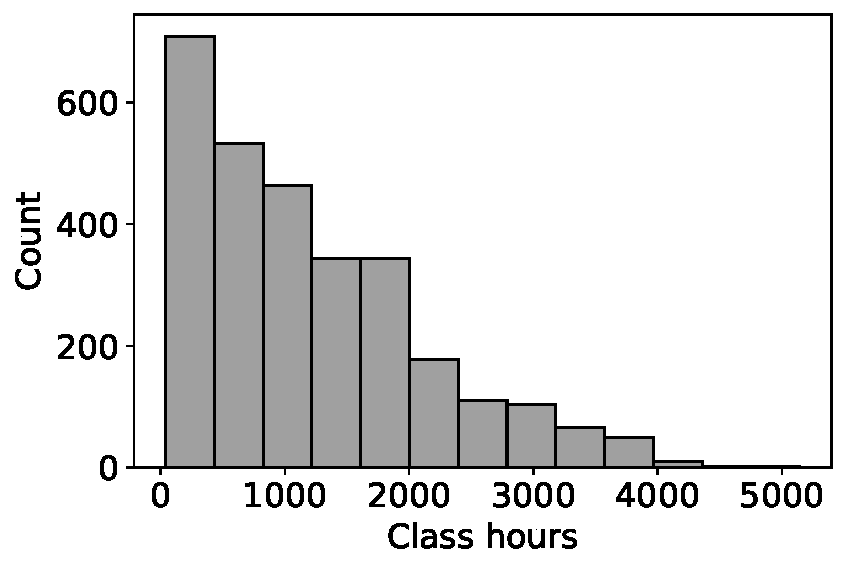
\includegraphics[width=\textwidth]{img/hist_dm_filter_bma.pdf}
         \vspace{-15pt}
         \caption{$D\geq 40$ and $Y>0$.}
     \end{subfigure}
     \hfill
     \begin{subfigure}[b]{0.45\textwidth}
         \centering
         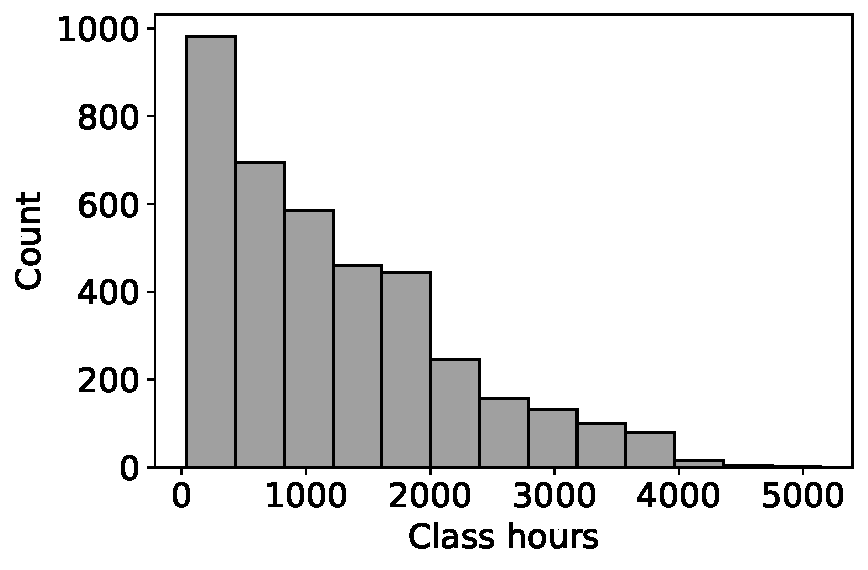
\includegraphics[width=\textwidth]{img/hist_d_filter_bma.pdf}
         \vspace{-15pt}
         \caption{$D\geq 40$.}
     \end{subfigure}
\par
\caption{\label{fig:hist}
Class hours for different samples.}
\end{centering}
\end{figure}


%\vspace{-5pt}
\begin{figure}[ht]
\begin{centering}
     \begin{subfigure}[b]{0.45\textwidth}
         \centering
         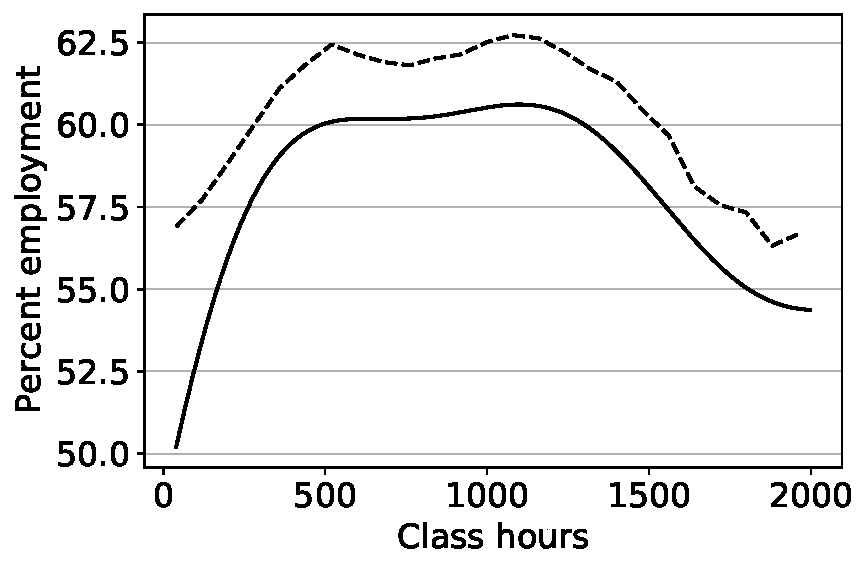
\includegraphics[width=\textwidth]{img/ATE_JCdata_dm_filter_with_dml_bma.pdf}
         %\vspace{-20pt}
         \caption{Dose response curve.}
     \end{subfigure}
     \hfill
     \begin{subfigure}[b]{0.45\textwidth}
         \centering
         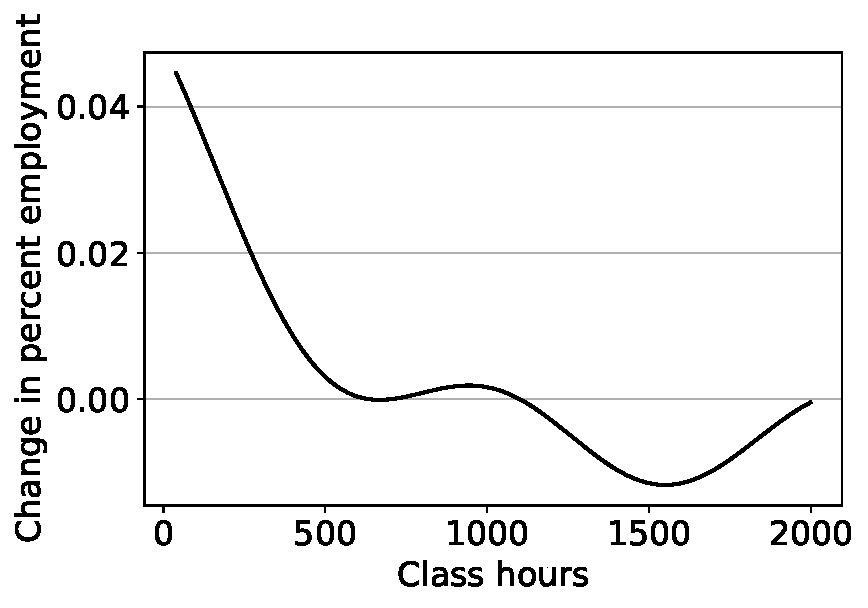
\includegraphics[width=\textwidth]{img/Incremental_ATE_JCdata_dm_filter_bma.pdf}
         %\vspace{-20pt}
         \caption{Incremental response curve.}
     \end{subfigure}
     \vskip\baselineskip
     \begin{subfigure}[b]{0.45\textwidth}
         \centering
         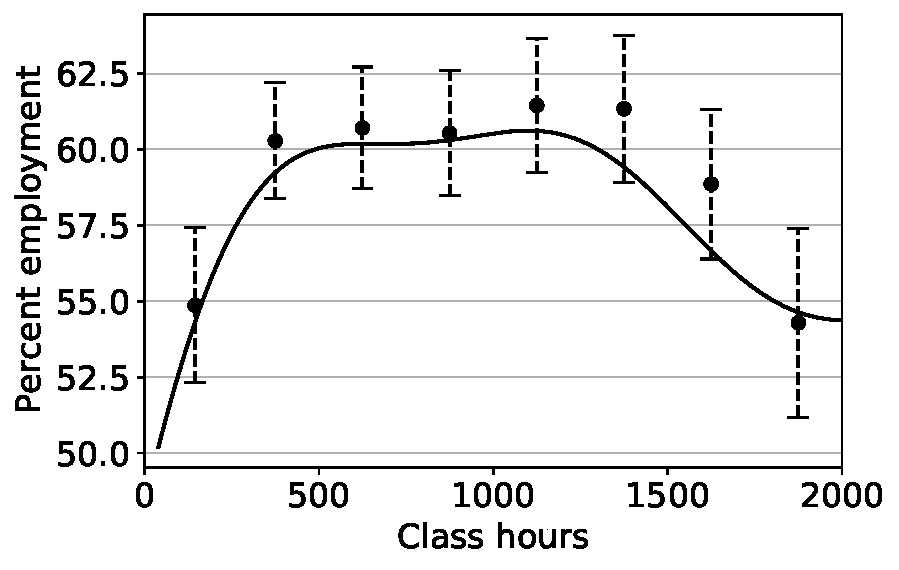
\includegraphics[width=\textwidth]{img/ATE_JCdata_dm_filter_ci_fine_gaussian2_bma.pdf}
         %\vspace{-20pt}
         \caption{Discrete treatment effects.}
     \end{subfigure}
     \hfill
     \begin{subfigure}[b]{0.45\textwidth}
         \centering
         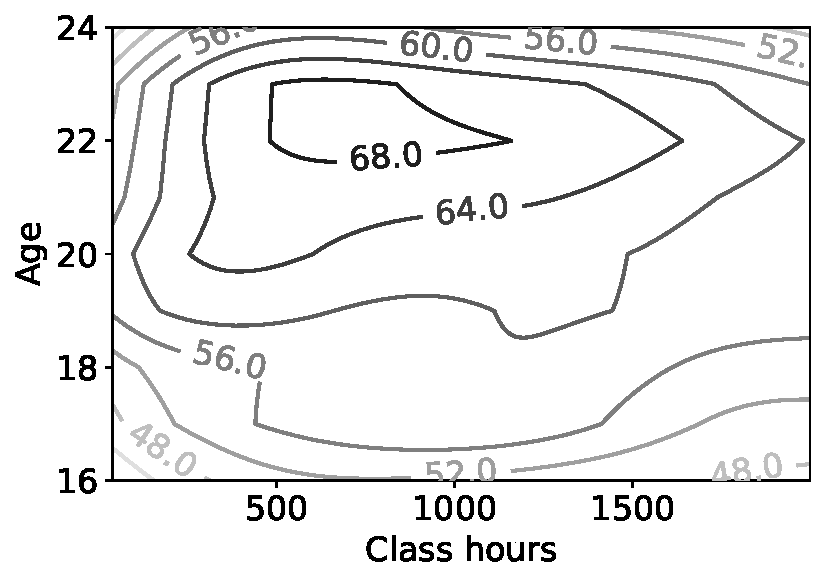
\includegraphics[width=\textwidth]{img/CATE_Age_JCdata_dm_filter_bma.pdf}
         %\vspace{-20pt}
         \caption{Heterogeneous response curve.}
     \end{subfigure}
\par
%\vspace{-10pt}
\caption{\label{fig:JC_d}
Effect of job training on employment: $D\geq 40$ and $Y>0$. We implement our estimators for dose, heterogeneous, and incremental response curves (\texttt{RKHS}, solid). For comparison, we also implement the dose response curve estimator of \cite{colangelo2020double} (\texttt{DR2}, dashes) as well as the discrete treatment effects of \cite{singh2021debiased} (\texttt{DR3}, vertical bars).}
\end{centering}
\end{figure}

We use the dataset published by \cite{huber2020direct}. In Supplement~\ref{sec:experiments}, we focus on the $n=3,906$ observations for which $D\geq 40$, i.e. individuals who completed at least one week of training. In this section, we verify that our results are robust to the choice of sample. Specifically, we consider the sample with $D\geq 40$ and $Y>0$, i.e. the $n=2,989$ individuals who completed at least one week of training and who found employment. 



For each sample, we visualize class hours $D$ with a histogram in Figure~\ref{fig:hist}. The class hour distribution in the sample with $D\geq 40$ and $Y>0$ is similar to the class hour distribution in the sample with $D\geq 40$ that we use in Supplement~\ref{sec:experiments}. Next, we estimate the dose, heterogeneous, and incremental response curve for the new sample choice. Figure~\ref{fig:JC_d} % and~\ref{fig:JC_full} 
visualizes results. For the sample with $D\geq 40$ and $Y>0$, the results mirror the results of the sample with $D\geq 40$ presented in Supplement~\ref{sec:experiments}. Excluding observations for which $Y=0$ leads to estimates that have the same shape but higher magnitudes, confirming the robustness of the results we present in Supplement~\ref{sec:experiments}. 


\end{document}
